%---------------------------------------------------------------------------%
%-                                                                         -%
%-                           LaTeX Template                                -%
%-                                                                         -%
%---------------------------------------------------------------------------%
%- Copyright (C) Huangrui Mo <huangrui.mo@gmail.com> 
%- This is free software: you can redistribute it and/or modify it
%- under the terms of the GNU General Public License as published by
%- the Free Software Foundation, either version 3 of the License, or
%- (at your option) any later version.
%---------------------------------------------------------------------------%
%->> Document class declaration
%---------------------------------------------------------------------------%
\documentclass[twoside]{Style/ucasthesis}%
%- Multiple optional arguments:
%- [<oneside|twoside|print>]% oneside eprint, twoside eprint, or paper print
%- [fontset=<adobe|none|...>]% specify font set instead of automatic detection
%- [scheme=plain]% thesis writing of international students
%- [draftversion]% show draft version information
%- [standard options for ctex book class: draft|paper size|font size|...]%
%---------------------------------------------------------------------------%
%->> Document settings
%---------------------------------------------------------------------------%
\usepackage[super,list]{Style/artratex}% document settings
%- usage: \usepackage[option1,option2,...,optionN]{artratex}
%- Multiple optional arguments:
%- [bibtex|biber]% set bibliography processor and package
%- [<numbers|super|authoryear|alpha>]% set citation and reference style
%- <numbers>: textual: Jones [1]; parenthetical: [1]
%- <super>: textual: Jones superscript [1]; parenthetical: superscript [1]
%- <authoryear>: textual: Jones (1995); parenthetical: (Jones, 1995)
%- <alpha>: textual: not available; parenthetical: [Jon95]
%- [geometry]% reconfigure page layout via geometry package
%- [lscape]% provide landscape layout environment
%- [xhf]% disable header and footer via fancyhdr package
%- [color]% provide color support via xcolor package
%- [background]% enable page background
%- [tikz]% provide complex diagrams via tikz package
%- [table]% provide complex tables via ctable package
%- [list]% provide enhanced list environments for algorithm and coding
%- [math]% enable some extra math packages
%- [xlink]% disable link colors
\usepackage{Style/artracom}% user defined commands
\usepackage{multirow}
\usepackage{booktabs}
\usepackage{float}
%---------------------------------------------------------------------------%
%->> Document inclusion
%---------------------------------------------------------------------------%
%\includeonly{Tex/Chap_1,...,Tex/Chap_N}% selected files compilation
%---------------------------------------------------------------------------%
%->> Document content
%---------------------------------------------------------------------------%
%-
%-> Titlepage information
%-
%---------------------------------------------------------------------------%
%->> Titlepage information
%---------------------------------------------------------------------------%
%-
%-> 中文封面信息
%-
\confidential{}% 密级:只有涉密论文才填写
\schoollogo[scale=0.095]{ucas_logo}% 校徽
\title{面向分布式图计算系统的自适应优化方法研究}% 论文中文题目
\author{陈军航}% 论文作者
\advisor{冯晓兵~研究员~\\中国科学院计算技术研究所}% 指导教师:姓名 专业技术职务 工作单位
%\advisor{指导教师一\\指导教师二\\指导教师三}% 多行指导教师示例
\degree{硕士}% 学位:学士、硕士、博士
\degreetype{工程}% 学位类别:理学、工学、工程、医学等
\major{计算机技术}% 二级学科专业名称
\institute{中国科学院大学人工智能学院}% 院系名称
%\institute{中国科学院力学研究所\\流固耦合实验室}% 多行院系名称示例
\date{2020~年~6~月}% 毕业日期:夏季为6月、冬季为12月
%-
%-> 英文封面信息
%-
\TITLE{Research on Adaptive Optimization Method for Distributed Graph Computing System}% 论文英文题目
\AUTHOR{Chen Junhang}% 论文作者
\ADVISOR{Supervisor: Professor Feng Xiaobing}% 指导教师
\DEGREE{Master}% 学位:Bachelor, Master, Doctor, Postdoctor。封面据英文学位名称自动切换,需确保拼写准确
\DEGREETYPE{Engineering}% 学位类别:Philosophy, Natural Science, Engineering, Economics, Agriculture 等
\MAJOR{Computer Technology}% 二级学科专业名称
\INSTITUTE{School of Artificial Intelligence,University of Chinese Academy of Sciences}% 院系名称
\DATE{June, 2020}% 毕业日期:夏季为June、冬季为December
%---------------------------------------------------------------------------%
%
\begin{document}
%-
%-> Frontmatter: title page, abstract, content list, symbol list, preface
%-
\frontmatter% initialize the environment
%---------------------------------------------------------------------------%
%->> Frontmatter
%---------------------------------------------------------------------------%
%-
%-> 生成封面
%-
\maketitle% 生成中文封面
\MAKETITLE% 生成英文封面
%-
%-> 作者声明
%-
\makedeclaration% 生成声明页
%-
%-> 中文摘要
%-
\intobmk\chapter*{摘\quad 要}% 显示在书签但不显示在目录
\setcounter{page}{1}% 开始页码
\pagenumbering{Roman}% 页码符号

随着大数据时代的到来,工业界和学术界开发了很多分布式图计算框架来对大规模图数据进行分析处理。
这些框架要正确处理顶点的副本点之间的数据一致性问题。
很多框架采用急切数据一致性(eager data coherency)的方法来解决这一问题。
这种方法把顶点的不同副本点看作一个不可分割的原子顶点,任何副本上的变化都要立即同步给其他副本,因而带来了频繁的全局同步和通信开销。
对此,我们在之前的工作中提出了一种称之为LazyAsync的方法。它基于延迟数据一致性(lazy data coherency)的思想,
顶点的不同副本点被看作互相独立的点,各自迭代更新,最后通过计算实现数据一致。
这种方法有效减少了系统中进行数据一致所引起的全局同步和通信,极大地提升了现有分布式图计算的效率。
然而,不同的开启策略会使LazyAsync得到不同程度的性能提升,
这使得LazyAsync只能通过手动调优来获得最大程度的性能提升。
至今仍没有行之有效的自适应优化方法解决LazyAsync的开启策略问题。

本文首先通过实验分析发现了不同开启策略对LazyAsync的影响程度主要受冗余计算的影响。
LazyAsync虽然避免了eager data coherency 方法中存在的冗余同步和通信,
但是在它的本地计算中存在着冗余计算。
冗余计算比例低的开启策略会得到更好的性能提升。
之后,本文通过离线分析发现了分布式图计算迭代过程中存在着解的局部性规律。
即点的全局解只由某个局部解构成,而解的局部性则有利于减少本地计算中的冗余计算。

最终本文针对LazyAsync设计并实现了一种基于解的局部性的自适应优化方法。
这种方法在线地统计顶点上全局解和局部解的关系识别出迭代过程中出现的解的局部性,
从而自适应地选择开启策略,自动得到相对最优的性能提升。
这种方法克服了之前的决策树方法需要事先繁重的手动调优的缺点,
并能有效处理决策树失灵的情况,使得LazyAsync成为了一种真正实用的方法。
在48机的集群环境下,这种方法相比于 eager data coherency 方法在4种典型图算法和不同种类输入图上
获得了和手动调优效果相一致的1.2到4.7倍的加速比。




\keywords{自适应优化,延迟数据一致性,图计算, 分布式计算}% 中文关键词
%-
%-> 英文摘要
%-
\intobmk\chapter*{Abstract}% 显示在书签但不显示在目录

With the advent of the era of big data, industry and academia have developed a number of distributed graph computing frameworks to efficiently analyze and process large amounts of graph data.
These frameworks have to properly handle data consistency between replication of vertex.
Many frameworks use approach of eager data coherency to solve this problem.
This approach treats the replication of the vertex as one indivisible atomic vertex, 
and any changes on the replication are immediately synchronized to the other replicas, 
thus incurring frequent global synchronization and communication overheads.
For this, we have proposed a method called LazyAsync in our previous work.
It is based on the idea of lazy data coherency.
The different replicas of the vertex are treated as mutually independent vertex, 
each iteratively updated, and finally the data is computationally coherence.
This method effectively reduces the global synchronization and communication caused 
by data coherency in the system, 
and greatly improves the efficiency of the existing distributed graph computation.
However, different turn-on strategies will give LazyAsync different levels of performance gains.
This leaves LazyAsync to be manually tuned for maximum performance gains.
There is still no proven adaptive optimization method to solve the problem of LazyAsync's turn-on strategy.

This paper firstly found through experiment analysis that 
the influence degree of different turn-on strategies on LazyAsync is mainly influenced by redundant computing.
LazyAsync avoids the redundant synchronization and communication in the eager data coherency method.
But there are redundant computation in its local computation.
A turn-on strategy with a low percentage of redundant computation yields better performance.
Subsequently, the offline analysis in this paper reveals that 
there is a pattern of localization of solutions in the iterative process of distributed graph computation.
The global solution of a vertex consists only of some local solution, 
and the localization of solutions helps to reduce redundant computations in local computations.

Ultimately this paper designs and implements an adaptive optimization method 
based on  the localities of  solutions for LazyAsync.
This method online statistically identifies the relationship 
between global and local solutions on vertices 
to identify the locality of the solution that emerge during iterations, 
thereby adaptively selecting the turn-on strategy and 
automatically obtaining a relatively optimal performance improvement.
This method overcomes the disadvantages of previous decision tree methods that required onerous prior manual tuning.
And the ability to effectively handle decision tree failures makes LazyAsync a truly practical approach.
In the cluster environment of 48 machines, this method is compared with the eager data coherency method 
on 4 typical graph algorithms and different types of input graphs.
Acceleration ratios of 1.2 to 4.7 times were obtained that were consistent with manual tuning results.

% 随着大数据时代的到来,工业界和学术界开发了很多分布式图计算框架来对海量的图数据进行高效地处理分析。
% 在这些框架中,顶点的副本点使得框架可以对单个顶点进行并行处理,并使不同机器上的邻居顶点在本地互相访问数据成为可能。
% 但是另一方面顶点的副本点也带来了数据一致性的问题。
% 为了维护副本点之间的数据一致,分布式图计算系统往往采用把顶点的所有副本点当作是一个原子的不可分割的点的急切数据一致性的方法。
% 然而,急切数据一致性方法给分布式图计算系统带来了频繁的全局数据同步和通信开销。
% 针对该方法存在的问题,一种把顶点的副本点看看作是互相独立的点各自独立迭代然后通过基于同样的差值消息进行计算得到相同视图的延迟数据一致性方法(lazy data coherency, LazyAsync)被提出。
% 这种方法可以有效减少系统中进行数据一致过程所需要的数据同步和通信,能够极大地提升现有分布式图计算的效率。
% 然而,不同的开启策略会使LazyAsync执行模式下的分布式图计算得到不同程度的性能提升,
% 这使得LazyAsync只能通过手动调优来获得最大程度的性能提升。
% 至今仍没有行之有效的自适应优化方法解决LazyAsync的开启策略问题。

% 本文提出了一种基于解的局部性的自适应优化方法,
% 它能够有效的针对不同环境自适应地选择开启策略使LazyAsync得到相对最优的性能提升。
% 我们首先通过具体的实验分析发现了不同开启策略对LazyAsync的影响程度主要受冗余计算的影响。
% LazyAsync方法虽然避免了急切数据一致方法中存在的冗余同步和通信,
% 但是在它的本地计算中存在着冗余计算。
% 不同的开启策略下存在着不同程度的本地冗余计算。
% 之后,通过离线分析,我们发现了分布式图计算迭代过程中存在着解的局部性规律。
% 即点的全局解只由某个局部解构成,而解的局部性则有利于减少本地计算中的冗余计算。
% 最终,通过在线地统计顶点上全局解和局部解的关系,
% 我们实现了一种在线的自适应优化方法。
% 它能够识别出迭代过程中出现的解的局部性,
% 并指导开启LazyAsync的策略,从而得到和手动调优效果一致的相对最优的性能提升。

% 本文主要针对LazyAsync方法进一步提出了一种基于解的局部性的自适应优化方法,
% 解决了LazyAsync不同开启策略性能提升不同的问题。
% 这种方法是一种在线统计方法,克服了之前的决策树方法需要事先繁重的手动调优的缺点,
% 并能有效处理决策树失灵的情况,使得延迟数据一致性方法成为了一种真正实用的方法。


% With the advent of the era of big data, industry and academia have developed a number of distributed graph computing frameworks to efficiently process and analyze large amounts of graph data.
% In these frameworks, the replication of vertices allows the framework to perform parallel processing on individual vertices, while also allowing neighboring vertices on different machines to access each other's data locally.
% But on the other hand the replication of vertices also poses data coherency problems.
% In order to maintain data coherency between the replication of vertices, distributed graph computing systems tend to use the method of treating all  replication of a vertex as if they were indivisible vertex of an atom with eager data coherency.
% However, the eager data coherency approach imposes frequent global data synchronization and communication overheads on distributed graph computing systems.
% To address the problems with this approach, one way that treats replication of vertices as if they were independent of each other and then computes them independently by exchanging delta messages to get the same view (lazy data coherency, LazyAsync) was proposed.
% This approach effectively reduces the data synchronization and communication required for data coherency in the system, thus greatly improving the efficiency of existing distributed graph computing.
% However, different turn-on strategy will result in different degrees of performance improvement for distributed graph computation in LazyAsync execution mode Elevation.
% This leaves LazyAsync to be manually tuned for maximum performance gains.
% There is still no proven adaptive optimization method to solve the problem of LazyAsync's turn-on strategy.

% In this paper, we present an adaptive optimization method based on solution localities.
% It effectively adaptively selects the turn-on strategy for different environments to achieve relatively optimal performance for LazyAsync.
% In this paper, it is 
% We first found through specific experimental analysis that the degree of performance improvement of the lazy data coherency method with different turn-on strategy is mainly influenced by redundant computing.
% The LazyAsync methods, while avoiding the redundant synchronization and communication that exists in the eager data coherency method, has redundant computations in its local computations.
% There are different levels of redundant computation under different turn-on strategies, which results in different levels of performance improvement.
% Subsequently, through offline analysis, we found that there is a pattern of localization of solutions in the iterative process of distributed graph computation.
% The global solution of a vertex consists only of some local solution, and the localization of solutions helps to reduce redundant computations in local computations.
% Ultimately, by counting the relationship between global and local solutions on vertices online.
% We implement an online adaptive optimization method capable of identifying the localities of  solutions that emerge during the iterative process.
% Then guide to turn on the lazy data coherency, resulting in relatively optimal performance gains consistent with manual tuning.

% In this paper, focusing on the LazyAsync method, we further propose an adaptive optimization method based on  the localities of  solutions ,
% solving the problem of performance improvement of LazyAsync with different turn-on strategies.
% This approach is an online statistical method that overcomes the disadvantages of previous decision tree methods that required onerous prior manual tuning.
% And the ability to effectively handle decision tree failures makes the lazy data coherency approach a truly practical approach.


% % 图是一种重要的数据结构。
% 随着大数据时代的到来,工业界和学术界开发了很多分布式图计算框架来对海量的图数据进行高效地处理分析。
% 在这些框架中,顶点的副本点扮使得框架可以对对单个顶点进行并行处理,同时也让不同机器上的邻居顶点在本地就可以互相访问数据。
% 但是另一方面顶点的副本点也带来了数据一致性的问题。
% 为了维护副本点之间的数据一致,分布式图计算系统往往采用把顶点的所有副本点当作是一个原子的不可分割的点的急切数据一致性的方法。
% 急切数据一致性方法给分布式图计算系统带来了频繁的全局数据同步和通信开销。
% 针对急切数据一致性的方法存在的问题,我们提出了一种把顶点的副本点看看作是互相独立的点各自独立迭代然后通过基于同样的差值消息进行计算得到相同视图的延迟数据一致性方法。
% 延迟数据一致性方法有效减少了系统中进行数据一致所需要的数据同步和通信,因而极大地提升了现有分布式图计算的效率。
% 但是这种方法还缺少一个合适的开启策略来得到相对最优的性能提升。

% 之前的工作中我们提出了一种基于决策树开启策略的自适应优化方法来解决这一问题,
% 但是决策树方法依赖于事先的手动调优产生合适的数据集,本质上是一种离线方法,
% 此外决策树方法对于训练集之外的算法和输入图组合存在失灵的情况。
% 因此决策树方法无法真正有效地解决延迟数据一致性的自适应优化问题。

% 在本文中,我们提出了一种基于解的局部性的自适应优化方法,它有效地解决了延迟数据一致方法如何得到相对最优的性能提升的问题。
% 延迟数据一致方法不同的开启策略会得到不同程度的性能提升。
% 本文先是通过具体的实验分析发现了延迟数据一致方法的性能提升的程度是受冗余计算的影响。
% 延迟数据一致方法虽然避免了急切数据一致方法中存在的冗余同步和通信,但是在它的本地计算中存在着冗余计算。
% 不同的开启策略下存在着不同程度的冗余计算因而得到了不同程度的性能提升。
% 接下来本文通过离线分析发现了图计算迭代过程中存在着解的局部性规律,即点的全局解只由某个局部解构成。
% 而解的局部性则有利于减少本地计算中的冗余计算。
% 最终通过在线地统计顶点上全局解和局部解的关系,
% 我们实现了一种在线的自适应优化方法能够识别出迭代过程中出现的解的局部性,
% 然后指导开启延迟数据一致,从而得到和手动调优效果一致的相对最优的性能提升。

% 在之前的工作中,我们针对分布式图计算框架在副本点上采用的急切数据一致性方法存在的频繁的冗余数据同步和计算这些问题
% 提出了一种延迟数据一致性方法,极大地提高了现有图计算的效率。
% 本文则进一步提出了一种基于解的局部性的自适应优化方法解决了延迟数据一致性方法遗留下的如何得到相对最优的性能提升的问题。
% 这种方法是一种在线统计方法,克服了之前的决策树方法需要事先繁重的手动调优的缺点,并能有效处理决策树失灵的情况,
% 使得延迟数据一致性方法成为了一个真正实用的方法。

% With the advent of the era of big data, industry and academia have developed a number of distributed graph computing frameworks to efficiently process and analyze large amounts of graph data.
% In these frameworks, the replication of vertices allows the framework to perform parallel processing on individual vertices, while also allowing neighboring vertices on different machines to access each other's data locally.
% But on the other hand the replication of vertices also poses data coherency problems.
% In order to maintain data coherency between the replication of vertices, distributed graph computing systems tend to use the method of treating all  replication of a vertex as if they were indivisible vertex of an atom with eager data coherency.
% The eager data coherency approach imposes frequent global data synchronization and communication overhead on distributed graph computing systems.
% To address the problem of the eager data coherency method, we propose a lazy data coherency method that treats replicate points of vertices as if they were independent of each other and then computes them independently by exchanging delta messages to get the same view.
% The lazy data coherency approach effectively reduces the data synchronization and communication required for data coherency in the system, thus greatly improving the efficiency of existing distributed graph computing.
% But this approach also lacks a proper turn-on strategy.

% In previous work we proposed an adaptive optimization method based on a decision tree turn-on strategy to address this problem.
% But the decision tree approach relies on prior manual tuning to produce the right data set and is essentially an offline approach.
% In addition, the decision tree method has failures for algorithm and input graph combinations outside the training set.
% Therefore, the decision tree approach cannot really effectively solve the problem of adaptive optimization for lazy data coherency.


% In this paper, we present an adaptive optimization method based on solution localities, which effectively solves the problem of how eager data coherency methods can obtain relatively optimal performance gains.
% Different turn-on strategies with different lazy data coherency methods result in different degrees of performance improvement.
% In this paper, it is first found through specific experimental analysis that the degree of performance improvement of the lazy data coherency method is influenced by redundant computing.
% The lazy data coherency method, while avoiding the redundant synchronization and communication that exists in the eager data coherency method, has redundant computations in its local computations.
% There are different levels of redundant computation under different turn-on strategies, which results in different levels of performance improvement.
% The next paper finds, through offline analysis, that there is a local law of solution in the iterative process of graph computation, i.e. the global solution of a vertex consists only of some local solution.
% And the local nature of the solution facilitates the reduction of redundant computing in local computing.
% Ultimately, by counting the relationship between global and local solutions on vertices online.
% We implement an online adaptive optimization method capable of identifying the localities of the solutions that emerge during the iterative process.
% Then guide to turn on the lazy data coherency, resulting in relatively optimal performance gains consistent with manual tuning.


% In previous work, we addressed these problems with frequent redundant data synchronization and computation of the eager data coherency approach adopted by the distributed graph computing framework at the replica vertex
% A lazy data coherency method is proposed that greatly improves the efficiency of existing graph calculations.
% This paper further proposes a solution-based localization adaptive optimization method that addresses the problem of how to obtain relatively optimal performance gains left over from the lazy data coherency method.
% This approach is an online statistical method that overcomes the disadvantages of the previous decision tree approach that required heavy manual tuning beforehand and can effectively handle decision tree failures.
% makes the lazy data coherency approach a truly practical one.

\KEYWORDS{Adaptive Optimization, Lazy Data Coherency, Graph Computing, Distributed Computing}% 英文关键词
%---------------------------------------------------------------------------%
% title page, abstract
{% content list region
\linespread{1.2}% local line space
\intobmk*{\cleardoublepage}{\contentsname}% add link to bookmark
\tableofcontents% content catalog
\intobmk*{\cleardoublepage}{\listfigurename}% add link to bookmark
\listoffigures% figure catalog
\intobmk*{\cleardoublepage}{\listtablename}% add link to bookmark
\listoftables% table catalog
}
% \input{Tex/Prematter}% symbol list, preface content
%-
%-> Mainmatter
%-
\mainmatter% initialize the environment
%---------------------------------------------------------------------------%
%->> Main content
%---------------------------------------------------------------------------%

% \input{Tex/Chap_Intro}
\chapter{引言}
\section{研究背景}
% 介绍图计算

%图计算很有用
图(Graph)是一种重要的数据结构,它由顶点与边构成。
如图\ref{fig:graph_important}所示,
图能够对很多问题进行抽象建模,
图计算在很多领域发挥了重要的作用。
比如在facebook、twitter、weibo这些社交网络中,我们可以把用户看作顶点,
把用户之间建立的关系看作边,这样就能用图来研究社交网络中的各种规律。
在互联网中通过把web网页看作顶点,
把页面之间的超链接看作边,就可以通过图来研究网页的权重排名信息。
而随着大数据时代的到来,如何对海量图数据进行高效的分析处理愈加成为工业和学术界的研究热点。

% 图(Graph)是一种重要的数据结构,它由顶点与边构成。
% 利用这种数据结构,我们能够对社交网络计算、广告、网页数据挖掘等各个方面进行抽象建模,从而获得有用信息(图\ref{fig:graph_important})。
% 在facebook、twitter、weibo这些社交网络中,我们可以把用户看作顶点,
% 把用户之间建立的关系看作边,从而进行社交网络中各种规律的研究。
% 在互联网中,我们通过把web网页看作顶点,
% 把页面之间的超链接看作边,利用这些信息研究网页的权重排名。
% 而随着大数据时代的到来,如何对海量图数据进行高效的分析处理愈加成为工业和学术界的研究热点。
\begin{figure}[!htbp]
  \centering
  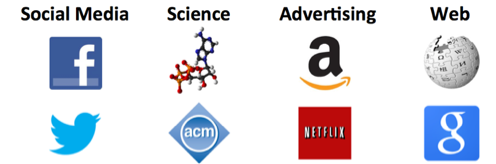
\includegraphics[width=0.40\textwidth]{graphs_are_everywhere.png}
  \bicaption{图计算的应用领域}{Application areas of graph computing}
  \label{fig:graph_important}
\end{figure}

%人们开发了很多框架进行图计算
传统的大数据处理平台使用MapReduce\cite{mapreduce}这种函数式编程范式,但这种编程范式并不适用于图计算。
基于函数式编程思想的MapReduce需要在每次迭代之间传递数据,
而图计算由于结构的内在复杂性,计算往往是不规则的,只有部分图数据参与计算,
那些不参与计算的数据在处理过程不需要传递。
此外图算法若要用MapReduce实现往往需要转换为一系列MapReduce任务,这又会带来额外的存储读写开销,
所以传统的大数据处理平台无法胜任大规模图计算任务\cite{Malewicz@SIGMOD10}。
为此人们开发了许多专门用于处理大规模图数据的分布式并行计算框架。    
\cite{Malewicz@SIGMOD10, Low@12, Gonzalez@OSDI12, Zhu@OSDI16, Gonzalez@OSDI14, Avery@HS11, Shao@SIGMOD13, 
Chen@EuroSys15, Xie@PPoPP15, Roy@SOSP15, Seo@CloudCom10, Gregor@POOSC15, Hoque@TRIOS13, Teixeira@SOSP15}

\section{针对副本点的延迟数据一致性方法}

%介绍副本点
当大规模图数据在集群中划分存储时,图中的顶点就出现了副本点。副本点在现有的分布式图计算编程框架中充当着关键角色。
它使得框架可以对单个顶点进行并行处理,并使不同机器上的邻居顶点在本地互相访问数据成为可能。
然而副本点在带来巨大好处的同时也引入了数据一致性的问题。\cite{Wang@PPoPP18, zlj2018}
分布式图计算编程框架要维护不同机器上存储的副本点$v_1, v_2, \cdots, v_k$之间的数据一致性。
% 这些图计算框架都要把大规模图数据在集群中分布式存储,因此副本点在现有的分布式图计算编程框架中充当着关键角色。  
% 副本点使得集群中的多台机器可以对一个顶点$v$并行地计算,同时也使得每个顶点可以在本地访问远程顶点,减少了机器之间的通讯开销。 

图\ref{fig:mirror}展示了一个小图在4台机器上划分后的结果,可以看到中心的顶点产生了4个副本点。
当4台机器并行计算改变顶点上的数据时,图计算要框架要负责维护这4个副本点之间的数据一致。

\begin{figure}[!htbp]
  \centering
  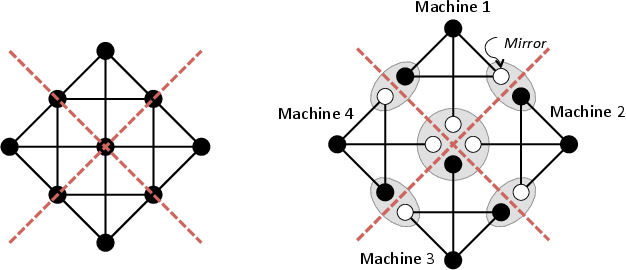
\includegraphics[width=0.40\textwidth]{mirror}
  \bicaption{副本点示意图}{schematic diagram of mirror vertex}
  \label{fig:mirror}
\end{figure}

%副本点存在的问题

很多编程框架都把每个顶点看做一个原子性的点,使用 eager data coherence 的方法来保证所有副本之间的数据是一致的,
每个点横跨的机器数量和数据同步频率直接影响系统通信量的大小进而影响系统的性能。
在这种方法中,系统把顶点$v$的副本点中的其中一个标记为master点,其他副本点为mirror点,其中master点保存了该顶点的真实数据,
而mirror点只实时地保存着master点数据的一份本地拷贝。
对顶点$v$的所有更新必须在master点上进行,更新完成后都会立即通过消息传递把最新状态发送给所有副本,这带来了频繁的全局同步和消息通信。

%lazygraph 的解决思路
针对这一问题,我们提出了一种延迟数据一致性方法(lazy data coherence,LazyAsync)\cite{Wang@PPoPP18}有效地降低了系统用于维护副本点数据一致性的开销。
我们发现,通过把算法每次迭代的公式改写为差值累加的形式,各副本点通过交换差值消息即可达到数据一致,
这样就消除了顶点计算过程中产生的数据同步和消息交换。
此外对于绝大多数图算法,系统时刻维护副本点之间的数据一致性并不是必须的。
对于一些经典的图算法某个点的解往往只依赖于它部分的邻居顶点,而对于数据挖掘和机器学习类的图算法中间过程的不一致往往不会影响最终的收敛性。
我们进一步通过数学公式推演证明迭代公式改写为差值累加的形式之后,
各副本点可以各自独立地进行数轮本地计算后再进行差值消息交换实现数据一致,
而不必在每次迭代之后就进行差值消息交换,它们最终得到的结果是等价的,
这样我们就可以进一步减少系统中进行数据同步和全局消息交换的开销。

%lazygraph 的效果
由于单个迭代计算过程中副本点之间不必同步,多轮迭代计算过程之间副本点之间可以延迟同步,
系统极大地减少了全局数据同步和通信的开销。
基于这些发现,我们把副本点看做是互相独立的迭代更新自己的数据的顶点,
% 各自进行数次迭代计算之后通过交换差值累加消息实现副本点之间的数据一致性
  各自进行数次迭代计算之后通过在同样的差值累加消息上进行计算来实现副本点之间的数据一致性,
并最终在具有代表性的分布式并行图计算框架PowerGraph\cite{Gonzalez@OSDI12}上实现了这种延迟数据一致性方法。
在48个虚拟机的EC2的集群环境下的实验结果表明,在4种典型的图算法和不同种类的真实输入图上,我们这种方法在保证正确性的基础上,
相较于PowerGraph获得了1.25倍到10.69倍的加速比。


\section{延迟数据一致性方法尚未解决的问题}
% lazygraph 的性能提升效果依赖于具体的延迟一致开启策略
% lazygraph 现在采用一个决策树模型作为开启策略,它存在着以下这些方面的不足
% 1. 难以解释
% 2. 训练过程依赖于手动调优
% 3. 无法做到自适应
虽然我们提出的延迟数据一致性方法极大地提升了分布式图计算的性能,但是它在以下几个方面还存在着一系列尚未解决的问题。    
\begin{enumerate}      
  \item[(一)] 延迟同步策略和系统得到性能提升相对大小之间的关系有待研究 \newline\indent
    何时开启延迟同步? 延迟同步开启多久进行数据一致? 
    随着这些具体策略的不同,系统得到的加速比也不同。
    要想得到相对最优的效果,研究清楚延迟同步如何影响性能提升是有必要的。

  \item[(二)] 目前系统实现的决策树方法存在缺陷 \newline\indent
    延迟数据一致性方法需要结合具体的应用算法和输入图选择合适的时间节点进行数据一致。
    目前的系统实现中采用的是通过离线训练得到的决策树模型,这种模型需要对算法和输入图组合手动调优,耗费时间较长,
    并且对于新的算法和输入图组合不能保证得到相对最优的性能提升,这对于一个实用的图计算系统来说是不可接受的。
    因此我们需要对目前的系统实现进行改进,把这个过程自动化,使得系统的模型具有足够的泛化能力,能够自适应的处理各种输入。          

  \item[(三)] 目前的系统缺乏一个考虑各种影响因素的自适应优化策略 \newline\indent
    %how to say?
    虽然我们提出了一种行之有效,且证明正确的延迟一致性方法,但是这个方法目前还缺乏一个自适应各种影响因素的优化策略。
    对于采用了延迟数据一致性的分布式并行图计算系统,除了延迟一致性开启策略之外,具体的算法用例,
    输入图结构特征,图划分算法,配置环境等都会对最终的性能造成影响,并且在系统执行过程中这些因素是动态变化而又互相影响的,
    为了得到相对最优的性能提升效率,系统需要一个能够自适应这些外部因素变化的优化策略,实时监控这些因素动态地调节全局同步的频率。          
    % 以及目前的系统实现中只在同步引擎上实现了延迟一致性方法,而有些算法更适合异步引擎,因此这种方法是否能够应用到异步引擎中也有待研究。
\end{enumerate}
\section{基于解的局部性的自适应优化方法}
% 通过实验发现, 解存在着局部性规律可以作为自适应开启策略
为了解决延迟数据一致性方法目前存在的问题,本文首先对这种方法的性能提升规律进行了研究。
在之前的工作中,我们从分布式计算系统的角度解释了延迟一致性方法的性能收益的来源。
延迟一致性方法减少了图计算的超步迭代次数,极大地降低了系统的全局同步等待和集群之间的通信这些开销,
从而得到了性能提升。
但是这种阐述只能说明延迟一致性方法方法能够提升性能这个定性的问题,
却无法回答延迟一致性方法在不同的开启策略下得到不同程度的性能收益这种定量的问题。
而且在实际的实验中我们发现,在某些情况下延迟一致方法虽然减少了迭代次数,但是最终却并没有拿到计算时间上的性能收益。

通过定义有效计算的概念,我们最终发现了延迟一致性方法的性能提升的相对大小的规律。
我们发现延迟数据一致性方法虽然避免了急切数据一致性方法中存在的冗余的同步,等待和通信,
但是却有可能在本地计算中引入新的冗余计算。
在延迟一致性方法不同的开启策略中,那些性能提升更好的情况是因为进行了更多的有效计算,
而那些性能提升相对不好的情况则是因为进行了更多的冗余计算。
所以,延迟一致方法要想得到相对最优的性能提升,就要从提高有效计算的比例入手。

通过分析,我们发现延迟一致方法能否进行更多的有效计算和顶点上的全局解和局部解的关系规律有关。
在分布式图计算中,由于副本点的存在,每个顶点上的全局解由多个局部解构成。
延迟一致性方法通过在数据一致性节点通过交换构成局部解的消息累加值来实现不同副本点上的全局解的一致。
而在数据一致性节点之间,各个副本点上在本地进行不需要消息交换和通信的本地计算。
这些本地计算能维持较高的有效计算的比例时,延迟一致性方法就能获得较高的性能收益。

另一方面,当顶点上的全局解只由一个局部解构成时,本地计算就能进行更多的有效计算,
当顶点上的全局解由多个局部解构成时,本地计算就容易造成更多的无效计算。
也就是说,当活跃点中的大多数点的全局解都只由单个局部解构成,
或者全局解由多个局部解构成的点的数量在下降时,
延迟一致性方法就能够通过多轮的本地计算对本地子图进行事先的有效计算,
最终得到较好的性能收益。


全局解和局部解的关系影响着延迟数据一致性方法的有效计算的程度,进而影响了这种方法的性能提升相对大小。
经过一系列实验之后,我们进一步找到了全局解和局部解的关系变化规律。
我们发现,在图计算过程中,随着计算的进行,全局解由多个局部解构成的点的数量会逐渐下降,
并且在每轮的活跃点中只占一小部分比例。
也就是说,随着计算的进行,图计算中的大部分顶点的全局解只由某一个局部解构成。
我们可以称之为解的局部性。
正是由于解的局部性的存在,延迟数据一致性方法才能通过延迟同步来减少系统中数据交换从而获得性能收益。

然而解的局部性并不是一直存在的,这也是延迟数据一致性方法需要合适的开启策略的重要原因。
通过实验我们发现,解的局部性和具体的输入图和算法用例以及集群的配置有关。
随着这些外部输入条件的不同,解的局部性也有着不同的变化规律。
在有的组合中,一开始就一直呈现出较为明显的解的局部性的规律,即全局解由多个局部解构成的顶点一直只占极少一部分。
而在有的组合中,一开始解的局部性现象并不存在,而是存在着全局解由多个局部解构成的顶点数量一直在增长的过程。
当这样的顶点数量在增长时,是不适宜开启延迟数据一致性方法的。

在之前的工作中,我们通过机器学习的手段找到了一个决策树模型作为开启策略。
这个决策树使用输入图的边点比例和运行时的活跃点变化趋势作为开启策略的判断条件。
通过实验我们发现,决策树所使用的特征其实也是对解的局部性变化规律的间接反映。
% 同时,由于决策树是对手动调优产生的训练集的数据拟合

最终,通过在运行时动态的监控全局解由多个局部解构成的顶点的数量和比例,我们得到了一个基于解的局部性的自适应优化方法。
这个自适应优化方法在动态观察到图计算迭代过程中开始存在解的局部性时,就开启延迟数据一致性方法。
这种方法克服了之前的决策树模型存在的失灵问题,同时也不需要事先的手动调优产生数据集来进行训练。
此外,由于解的局部性是受输入图特性,算法用例,集群配置环境所共同影响的,所以这种方法能够实现对这些不同外部输入条件的自适应。

总而言之,本文的主要创新点和贡献可以归纳为以下几点:

1. 对延迟数据一致性方法的在不同开启策略下得到不同性能提升这一现象进行了研究,认清了这一方法的性能提升规律。
以具体的例子识别出了延迟数据一致性方法虽然避免了急切数据一致性方法存在的冗余同步和通信,但是引入了新的冗余计算。
并且正是这种冗余计算造成了延迟数据一致性方法在不同开启策略性下得到不同程度的性能提升。

2. 对图计算过程中活跃点上全局解和局部解之间的关系进行了研究,发现了解的局部性这一现象。
通过分析,本文发现随着图计算的进行,每次迭代中大部分活跃点的全局解只由某个局部解构成,
那么此时局部解所在的副本点完全不需要等待和同步其他副本点就可以继续进行图计算过程。
而这种情况正是有利于减少冗余计算,有利于开启延迟数据一致性方法的情况。

3. 基于解的局部性这一现象,设计并实现了基于解的局部性的自适应优化方法。
这种方法解决了延迟数据一致性方法在不同的输入条件下如何得到相对最优的性能提升这一问题。
相较于之前采用的决策树方法,这种方法不需要事先的离线调优和训练,更不存在某些输入条件下失灵的问题。


%从 到 最终 我们发现了。。。


\section{全文结构}
% 每一章写了什么
本文各章节的具体内容安排如下:

第一章是引言。介绍了我们之前针对分布式并行图计算框架中副本点存在的问题所提出的延迟数据一致方法这一研究背景。
然后介绍了这个方法所遗留的问题,以及本文针对这些问题所做的工作。

第二章是相关技术介绍及研究动机。介绍了分布式图计算中主要的研究主题,并对本文的研究基础-延迟数据一致性方法做了重点介绍。
随后介绍了延迟数据一致性的开启策略问题,也正是本文的研究动机。

第三章LazyGraph性能提升规律研究。
首先对延迟数据一致性方法的性能收益的来源进行了研究。
从具体算法的角度,本文展示了这种方法的性能收益来自于 它能够在本地计算所进行的额外多轮迭代中提前激活顶点并使之收敛。
然后通过分析具体的例子,本文提出在这种本地计算中存在着冗余无效的计算,并且这些冗余计算会造成性能损失。
最后本文通过具体的实验验证了这一观点。
从延迟一致带来的性能收益,到冗余计算带来的性能损失,本文在这一章发现LazyGraph不同开启策略下得到不同程度的性能提升这一现象
背后的原因
正是因为本地计算中存在着相应的不同程度的冗余计算。

第四章基于解的局部性的自适应优化方法。
冗余计算影响影响收益,
本章先是介绍了全局解和局部解的关系如何影响冗余计算。
然后通过离线分析的方法,本章对不同算法和输入图上全局解和局部解之间的关系进行了实验分析,
发现了全局解和局部解之间存在着局部性关系。
接下来通过在线统计的方法,本章提出了基于解的局部性的自适应优化方法用于指导延迟数据一致性的开启策略。
最后,本章在不同算法和输入图上进行了实验评测,并对评测结果进行了分析。

最后一章对全文的研究内容进行了总结和展望。





\chapter{相关技术介绍及研究动机}
\section{分布式并行图处理框架}
% 由于MapReduce编程范式存在着进行多轮迭代图计算时带来中间结果存储开销,实现图算法需要额外转换等问题,
% 人们在并行分布式处理大规模图数据过程中广泛使用BSP(Bulk Synchronous Parallel)模型\cite{bsp@1990}。
在对大规模图数据进行分布式并行处理时,BSP(Bulk Synchronous Parallel)模型\cite{bsp@1990}比MapReduce更为合适。
BSP模型由图灵奖得主Valiant于1990年提出,
它是一种基于消息通信的并行计算模型。
它的核心思想是将一个巨大复杂的计算任务分解为一系列的迭代运算,因此尤其适合做数据的迭代计算。
如图\ref{fig:bsp}所示,一个BSP作业由若干个顺序执行的超步(super step)组成:$S_1,S_2,\cdots,S_n$,对应于$n$次迭代处理。
并行计算的任务按照超步进行组织,在超步$S_i$内,各任务异步接受来自$S_{i-1}$的消息,执行本地计算并发送消息给下一个超步$S_{i+1}$。
BSP模型对相邻的超步进行同步控制,确保超步$S_i$内的所有任务均已完成才进入下一个超步$S_{i+1}$,这种同步方式可避免死锁和数据竞争问题。
与MapReduce相比,BSP这样的运行逻辑避免了由于多次迭代产生的数据反复迁移和作业连续调度的问题,从而可以使得迭代处理更加灵活,
更加适合处理图计算问题。
\begin{figure}[!htbp]
  \centering
  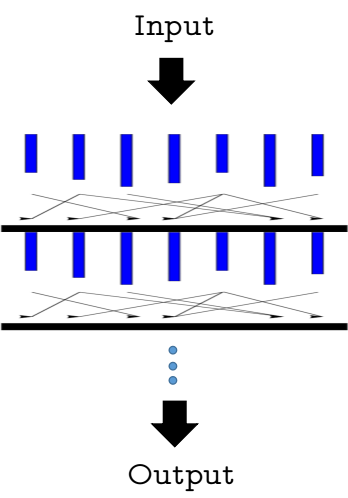
\includegraphics[width=0.40\textwidth]{bsp}
  \bicaption{BSP模型}{bsp model}
  \label{fig:bsp}
\end{figure}

受BSP计算模型的启发,Google在2010年首次提出了以顶点为中心的分布式图计算框架Pregel\cite{Malewicz@SIGMOD10}。
自Pregel之后,围绕着Pregel存在的局限性,以及新的问题和需求,人们又开发出了一系列新的用于处理大规模图数据的分布式并行计算框架。
这些框架分别在任务调度机制,通信机制,图划分,计算粒度与顶点计算模型这四个方面上存在着不同\cite{TLV, reviewruc}。

\subsection{任务调度机制}
任务调度主要解决如何按照一定的规则对计算资源进行分配的问题。
在分布式图计算中,为了确保负载均衡避免木桶效应,任务调度问题必须得到有效的解决。
根据迭代计算过程系统中是否有多个超步在同时运行,
分布式图计算框架采用的任务调度机制可以分为同步调度,异步调度和混合调度这三类。

同步调度模式,指对两个相邻的超步$S_i$与$S_{i+1}$,必须在$S_i$超步结束之后才能够进入下一个$S_{i+1}$超步,
任何时刻系统中不存在两个交错运行的超步。
这种模式之下,下一个超步$S_{i+1}$执行运算时所看到的数据必然是上一个超步$S_i$的所有顶点执行完成之后的结果数据。
这种调度模式由于控制机制比较简单,因而便于用户理解及操作。
利用同步模式的分布式图计算框架运行图算法时,由于运行的过程直观明了,运行结果具有确定性,
因而有助于程序的设计,调试。
然而,这种调度模式下,由于在处理相同的超步$S_i$时,
不同计算顶点的处理能力不同,同时处理的图数据划分不均匀,
因而各个顶点执行计算所需的时间存在显著差异,从而产生木桶效应,
导致运行总时间过长,造成计算资源的浪费。
同时,由于在这种模式下,数据的传输只能发生在两次相邻的超步$S_i$和$S_{i+1}$之间,
有一定可能会造成在某些运行场景下运行结果始终无法收敛。
为解决同步调度模式中的这些问题,研究人员进一步提出了异步调度模式和混合调度模式


在异步调度模式中,前后两次超步$Si$和$S_{i+1}$之间没有明确的界限,
前一步$Si$中较为活跃的图顶点只要接收到其需要的消息,不必等待其他所有图顶点完成,
便可以自由地接受调度器的调度执行下一步操作,并向其他图顶点广播其完成的结果数据。
这一模式摒弃了数据传输和执行只能在相邻两超步$Si$与$S_{i+1}$之间的同步路障(barrier),
因而能够有效降低木桶效应,提供图计算的运行效率,同时解决某些算法在同步模式下无法收敛的问题。
然而,基于这一模式的分布式图计算框架在设计上较基于同步调度模式的分布式图计算框架要复杂许多,
系统设计时的编程难度也相应增加,需要设计出合适且高效的调度器。
同时在运行过程中可能出现异步计算过程中对数据的读写访问冲突,
计算过程和结果不确定等问题,运行需花费更多的精力反复就行修改调试。

在深入分析比较同步与异步调度模式之后,
许多分布式图计算框架中,将两者结合起来的混合调度模式被提出。
不同的混合调度模式实际上针对不同顶点和不同计算阶段分别切换同步和异步调度模式。
PowerSwitch\cite{Xie@PPoPP15}是比较有代表性的采用混合调度模式的系统。
它能够通过一组启发式算法建立一个代价收益模型,动态预测两种调度模式的性能,
并自由切换为性能最佳的调度模式,从而提高图计算的执行效率。

\subsection{通信机制}

通信机制,即分布式图计算框架中各个计算结点之间信息交流的方式。
当信息量过大时,信息传递的途径对分布式图计算系统的运行速度有着重要的影响。
分布式图计算框架目前常用的通信方式主要有基于共享内存和基于消息传递两大类。

基于共享内存通信的方式构建的分布式图计算框架中,
每个图顶点上的数据以共享变量的方式存储在计算机节点中,
其他图顶点可以通过框架提供的数据结构按照内存地址来快速读取。
然而在实际的应用中,
由于每个计算结点都有自己独立的内存地址空间且需要保证数据的一致性,
所以基于共享内存的通信机制实现起来较为困难。

基于消息传递的通信方式在实际上更为容易。
比较常用的网络通信协议有
RPC(remote procedure call)\cite{rpc}、Netty\cite{netty}、ActivMQ\cite{activemq}以及基于 MPI(message Passsing interface)\cite{mpi}
这几类。
在基于消息传递的通信机制中,
图顶点之间的信息交流通过网络通信平台在计算机节点间传送包含数据和目标顶点的ID的消息。
在这种方式中,系统会使用批量发送的方式来优化网络通信。
具体的方式为:若目标图顶点与发送消息的源顶点位于同一台机器上,
则直接将信息发送给相应的图顶点;
否则,消息将置于系统的消息发送缓冲池中,等待集中批量发送。
消息传递中的缓冲批量发送虽然能提供通信负载但同时也会因为消息的滞后而影响图计算的性能。


通信开销会严重影响整个分布式图处理系统的性能,
因此如何对基于消息传递或基于共享内存的通信方式进行优化
成为分布式图计算系统性能研究的重要任务。
现如今主要的优化方法主要从减少消息数量的角度进行入手:
一种是将图进行合理分割,降低图分区间的连通性,
从而降低跨机器的通信请求,从根本上减少跨机器的消息数量;
一种是通过将发送到相同目的顶点的消息合并成一条,
或者合并发送到相同机器的消息,从而减少消息的数量。


在系统进行消息传递通信的过程中,根据信息的流向,分布式图计算框架的工作模式可以划分为 push 模式和 pull 模式两种类型。

在 push 模式中,图中的活跃顶点完成计算产生数据信息后,随即发送给即将被激活的邻居顶点。
这种模式在内存资源充足的情况下可以减少数据传送时间,从而提高图计算效率。
然而在数据量较大的情况下,过多的数据信息存储会增加系统内存的压力。
而在pull模式下,只有图顶点需要某数据信息时才会主动向其他顶点请求数据,
从而避免了存储大量冗余的信息,减少了系统内存的压力。
这种模式下需要采取方法减少跨机器的消息数量,减少额外的通信开销。

两种模式各有利弊,分别适合不同的场景。
有不少研究工作通过混合使用两种模式来进一步提高图计算的执行效率。
单机图计算系统Ligra\cite{Shun@PPoPP13}混合采用push 和 pull 两种模式,
根据需要参与计算的活跃点的边数在两种模式间自适应地切换。
Gemini\cite{Zhu@OSDI16} 则将
在分布式环境中实现了这种双模式计算引擎,
并且进一步将两种模式下的计算过程都细分成发送端和接收端两个部分,
从而将分布式系统的通信从计算中剥离出来。

\subsection{图划分}

图数据划分是进行分布式图计算的基础,划分的合适与否直接影响着分布式图计算框架的性能。
在图划分过程中有两个要遵循的重要原则:一个是降低划分后子图之间的连通性,从而降低网络开销;
另一个是保证子图大小均匀,以实现系统的负载均衡\cite{reviewruc}。
图计算框架中的图划分技术可以从\textit{图划分方式和图划分策略}两个方面进行论述。

在分布式图处理系统中主要有两种图划分方式:
边切分方式(vertex-cut)\cite{Gonzalez@OSDI12}和点切分方式(edge-cut) \cite{Malewicz@SIGMOD10}。
边切分对顶点之间的边进行切分,即划分过程是把顶点分配到不同的计算结点上,然后在计算结点的子图内
把顶点之间的边补上去,划分后,被切断的边将出现在两个不同的子图中。
点切分是对图的节点进行切分,即划分过程是把边分配到不同的计算结点上,
划分后,每条边出现且仅出现在一个子图中,邻居多的点将会出现在多个子图中。

分布式图计算处理系统的图划分策略主要有 3 种: 
离线划分策略\cite{metis}、流式划分策略\cite{tsourakakis2014fennel}以及动态重划分策略\cite{kumar2017graphsteal} 。
离线划分策略在图数据被分布式图计算框架加载之前便将其划分为若干子图。
流式划分策略指在数据加载过程中对图数据边加载边划分。
这种策略假定数据以节点流或者边流的方式加载,根据已经到达数据的分布信息,建立一组启发式的规则,
从而决定已到达图数据的划分。
动态重划分策略首先收集系统运行过程中的状态数据,然后根据收集到的状态信息建立相应的模型,
指定划分策略,最后根据制定的策略进行划分。

\subsection{计算粒度与顶点计算模型}

粒度(Granularity)指在求解问题时研究对象的细致程度。
从不同的粒度对问题进行分析,有助于从不同角度对问题进行求解。
目前主要的分布式图计算处理系统分别以顶点、以子图或以路径作为计算粒度对图数据进行处理。
    
在以顶点为计算粒度的分布式图处理系统中,
迭代处理过程主要对图顶点进行遍历。
这种模式由于逻辑简单且具有良好的算法表达能力,
因而被绝大多数框架如GraphLab\cite{Low@12}、GraphX\cite{Gonzalez@OSDI14}、Giraph\cite{Avery@HS11}等采用。
不过该模式牺牲了图顶点访问子图内其他顶点信息的灵活性,因此存着着收敛速度过慢,网络通信量大等缺点。

针对以顶点为计算粒度模式的缺点,人们又提出了大量以子图为计算粒度的分布式图处理系统,
如GraphHP\cite{su2016graphhp},GoFFish\cite{goffish}等。
这种模式先对子图的边界点进行处理,然后接着处理子图内部的节点。
%不过这种模式表达能力较弱,因此不能够取代以顶点为粒度的模式。

以路径为计算粒度的模式主要在单机集中式图处理系统中使用,这种模式将边数据和点数据进行分区,
对边采用顺序访问的方式进行遍历计算,减少了对边数据的随机访问,进而降低了磁盘访问开销。
目前为止,在分布式环境下以路径为计算粒度的模式还缺少有效实践,不过这种模式可以为分布式图计算框架中的某些优化提供借鉴意义。

绝大多数分布式图处理系统以顶点为计算粒度,用户需要以图中的顶点为粒度定义运算函数。
在实现运算函数的时候,人们采用的是“Think Like A Vertex”\cite{TLV}这种编程思想。
% 这个运算函数的功能包括消息的收发、节点值的更新以及顶点状态
% 的改变等。然后,系统按照该运算函数对图中的每一个顶点进行同步或者异步的更新运算。      
这种编程思想以顶点为中心,从顶点的角度出发去描述图计算过程中每个顶点的行为。
在编程框架的迭代过程中,图中所有顶点不断地执行用户定义的顶点程序(vertex program),每个顶点只能从邻居顶点发送或接收消息,
当顶点收到消息后就处于激活状态,图计算的过程就是维护和更新每个顶点的状态的过程,当所有顶点都已经处于非激活状态,系统结束计算过程。
在具体实现过程中,计算框架主要把顶点程序分解为一个,两个或三个执行阶段。

单执行阶段的顶点程序可以用一个计算函数来表示,这个计算函数遵循这样的执行流程:访问邻居数据和消息,计算新的顶点状态值,分发状态变化值。
Pregel是采用了这种顶点程序抽象的一个典型代表。
两阶段的顶点程序常被分解为 Scatter-Gather 两个函数,并被称之为 Scatter-Gather 模型,
其中scatter阶段用于把顶点值分发给顶点,gather阶段用于收集输入然后用于执行顶点更新,
GraphChi\cite{GraphChi}使用Scatter-Gather作为标准的编程模型。
此外GRE\cite{GRE}编程框架也提出了一种在消息传递中使用的两阶段编程模型,Scatter-Combine,这种方法在活跃消息中既传递数据也传递操作。

PowerGraph\cite{Gonzalez@OSDI12}提出了一种三阶段执行过程的顶点程序,Gather-Apply-Scatter (GAS)。
Gather阶段对所有输入顶点或边上的消息进行求和,这个结果在Apply阶段用于更新顶点的状态,Scatter阶段把更新的消息传播出去。
PowerGraph是由共享内存架构的GraphLab\cite{Low@12}发展而来的,它既支持基于BSP实现的同步引擎,也支持采用灵活调度策略的异步引擎。
PowerGraph通过GAS的顶点编程模型配合vertex-cut的图划分方法,提高了图并行处理的粒度,较好地解决了图的幂律分布带来的计算不平衡问题。
在PowerGraph的vertex-cut划分方法中,图按边划分,每条边被唯一地分配到某个机器上去,顶点则在机器之间存在副本。
迭代过程中,每个顶点的副本能够互相独立的执行本地的gather阶段,然后各个副本把执行结果发送到指定好的master顶点上,
master顶点使用这个结果来执行完Apply阶段后把结果再发送给各个副本,然后各个副本又可以独立地执行本地的scatter阶段。


\begin{figure}[!htbp]
\centering
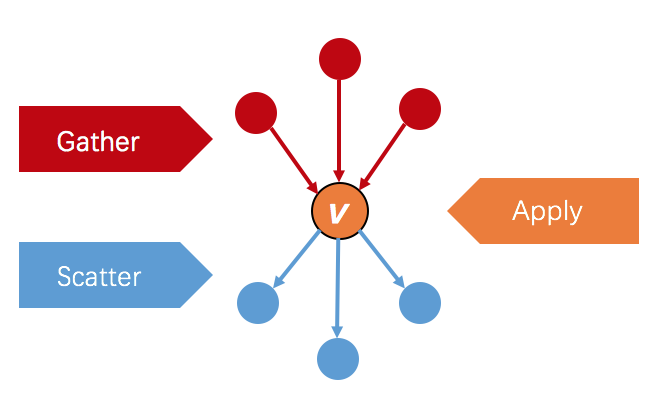
\includegraphics[width=0.40\textwidth]{gas_user}
\bicaption{用户视图下的GAS模型}{GAS Model in User View}
\end{figure}

在GAS的编程模型中,副本点的存在使得分布式图计算框架可以对单个顶点进行并行处理,并使不同机器上的邻居顶点在本地互相访问数据成为可能。
但是副本点也带来了数据一致性和副本点之间的消息传递问题,这些问题会在迭代计算过程中带来频繁的全局同步和通信开销,
LazyGraph\cite{Wang@PPoPP18}提出了一种 延迟数据一致性方法(LazyAsync),它基于
延迟数据一致性(lazy data coherency)的想法,将一个顶点的不同副本当作是独立的顶点,
它们可以维护和更新自己的数据,各自独立地进行本地计算,系统会选择合适的时间节点在副本点之间进行全局消息交换然后通过计算来使得它们达到数据一致,
这种方法消除了顶点计算过程中用于维护副本点之间的数据一致性所引起的各种消息传递的开销,减少了副本点之间消息交换的次数,极大地减少了系统中全局同步的次数和网络通信量。
副本点之间进行全局消息交换的时间节点直接影响着系统的性能,LazyGraph使用机器学习模型训练出的参数选择具体的时间节点。

% 自Pregel之后,研究者们使用各种优化手段提出了众多的分布式图计算框架。
% 这些框架大多数都对同一个顶点的不同副本点采取 eager datacoherency 的方式,因此带来频繁的全局同步和通信。 
% LazyGraph 采用 lazy data coherency 的方法来解决这个问题。
% Hieroglyph\cite{ju2017hieroglyph}也同样使得同一顶点的不同的副本点可以独立本地更新自己的数据。
% 但是,Hieroglyph关注于将计算从通信中解耦出来,以获得充足的本地计算,并且需要用户定义模块来解决数据一致性的问题。
% 而 LazyGraph 则关注于延迟副本点间的数据一致性,并同时减少全局同步次数和网络通信,并且在编程框架内部自动地维护副本点之间的数据一致性。
% 因此现有的研究不能直接用于处理我们提出的延迟数据一致性方法中遗留的几个问题。

\section{基于延迟数据一致性方法的 LazyGraph 图计算系统}
\subsection{顶点副本的延迟数据一致性方法}
% 延迟数据一致方法是什么

% 副本点
副本点在分布式并行图计算框架中发挥了巨大作用。
一方面它可以使得集群的多台机器对一个顶点进行并行处理,提高了计算效率。
另一方面,副本点使得顶点能够在通过本地内存直接访问那些被划分在远程机器的顶点,减少了通信开销。
图\ref{fig:graph_cut}给出了一个图在三台机器上分别进行点划分和边划分的结果。
可以看到图中的顶点划分之后产生了副本点。
以边划分为例,图\ref{fig:edge_cut}中C顶点在2号机器上有一个副本,
这使得系统可以对C顶点的两条边C-B和C-D进行并行处理。
此外,由于C顶点在2号机器上的副本点的存在,2号机器上的B顶点在访问它的邻居C顶点时可以从本机内存中直接访问,
而不必通过网络请求从3号机器上访问。



\begin{figure}[!htbp]
  \centering
  \begin{subfigure}[b]{0.35\textwidth}
    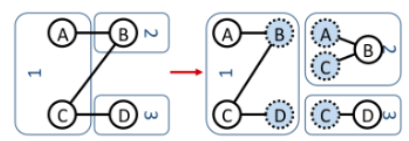
\includegraphics[width=\textwidth]{vertex_cut}
    \caption{}
    \label{fig:vertex_cut}
  \end{subfigure}%
  ~% add desired spacing
  \begin{subfigure}[b]{0.35\textwidth}
    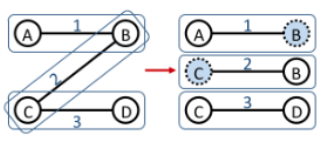
\includegraphics[width=\textwidth]{edge_cut}
    \caption{}
    \label{fig:edge_cut}
  \end{subfigure}
\bicaption{点划分和边划分}{vertex-cut and edge-cut}
\label{fig:graph_cut}
\end{figure}

% eager data coherence 及其 冗余

副本点在带来巨大好处的同时也引入了数据一致性的问题。
对于一个顶点在集群中同时分布存在的多个副本,之前的多数分布式图计算编程框架都采用 急切数据一致性(eager data coherency) 的方式来维护
这些副本之间的数据一致。
这种方式要求对顶点的任何修改都要在下一次新的修改之前同步到其他所有副本上。
图\ref{fig:pg-eager}展示了典型的图计算框架PowerGraph是如何实现 eager data coherency 的。
在PowerGraph的实现方式中,顶点的多个副本中某一个被标记为 master 点。对顶点的修改只在 master 点上进行,
修改之后把master 点的最新状态通过网络同步拷贝到其他副本点上。

\begin{figure}[!htbp]
  \centering
  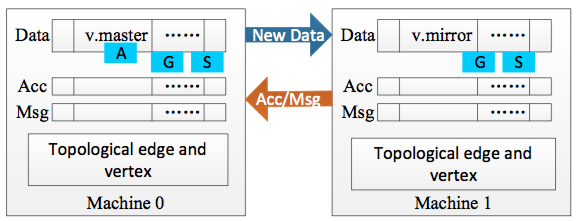
\includegraphics[width=0.40\textwidth]{pg-eager}
  \bicaption{PowerGraph 的 eager data coherency 实现\cite{Wang@PPoPP18}}{Eager Data Coherency in PowerGraph}
  \label{fig:pg-eager}
\end{figure}

eager data coherency 方式虽然最大程度地维护了顶点上数据的一致性,但是却带来了大量的冗余。
由于副本点上的数据必须从 master 上拷贝而来,因此在 master 上的数据进行修改时副本点上无法进行计算,
这带来了冗余的等待。
同时,由于master点上的数据必须通过网络同步拷贝给其他机器上的副本点,系统中因此引入了大量频繁的全局同步和通信。

% lazy data coherence 的方法
针对 eager data coherency 存在的问题,我们提出了一种称之为 LazyAsync 的延迟数据一致性方法,
并通过对通信机制和图加载划分等方面的其他工作把这个方法完善为了一个图计算系统LazyGraph\cite{Wang@PPoPP18}。
这种方法在保留副本点带来的好处的同时避免了 eager data coherency 方法存在的各种冗余问题。
在 LazyAsync 方法中,每个副本点都被当作一个独立的顶点,并且各自可以拥有自己的本地数据。
顶点在不同机器上的副本点分别维护着自己不同的本地视图,并且基于公式
$x_{i}^{t+1}=x_{i}^{t}+_{o p} \oplus_{j \rightarrow i \in E} \Delta_{j}^{t}$
进行迭代更新。
虽然不同的副本点它们收到的消息的次序不一致,但是只要有相同的初值和消息和,它们最终能够得到一致的值\cite{zlj2018}。

LazyAsync 将副本点 $v_1 , v_2 , \cdots , v_k$ 的计算过程分为本地计算和数据一致性两个阶段。
其仅仅在数据一致性阶段将各自的本地消息和其它副本点的远程消息进行合并,再通过计算实现数据一致。
因此,LasyAsync 的模式使得副本点在相邻两个数据一致性点之间维护各自不同的本地视图,
并在数据一致性阶段通过计算得到一致的全局视图。


LazyGraph 保留了现存分布式图计算编程框架的编程接口,同样使用GAS模式,
但是,需要用户将原来顶点程序改为 push-style 模式并支持 deltaMsg 消息传递\cite{zlj2018}。
和现存的分布式图计算编程框架一样,在有向图$G = \{V, E\}$上用户定义一个顶点程序 P,然后图中所有顶点$v \in V$并行地在多台机器上进行计算。
顶点之间的通信直接通过给对方发送消息来完成。一个顶点可以接受其它点发送过来的消息,然后修改自己的数据,再发送消息给其它顶点。
而图中的边用来传输数据。


当然,LazyAsync 也和现存的分布式图计算编程框架存在区别。
LazyAsync 要求顶点的迭代计算是可以用公式 $x_i^{t+1} = x_i^t +_{op} \oplus_{j \rightarrow i \in E} \Delta_j^t$ 来表示,
其中,$i$为顶点的 id 号,$t$为迭代计数器,$+_{op}$和$\oplus$表示运算符,$\Delta_j^t$表示顶点$j$在第t次迭代的消息变化值(deltaMsg)。
此外,$\oplus$是由用户定义的消息累加的运算符,LazyAsync 要求它必须是可交换且可累加的。
在 Gather 阶段,顶点$i$收到邻居点发送给它的消息$\Delta_j^t$,然后用$\oplus$操作进行累加求和,得到累加和 accum。
然后在 Apply 阶段,中心点用自己的数据和刚刚求得的累加和 accum 进行迭代更新$x_i^{t+1} = x_i^t +_{op} accum$。
最后,在 Scatter 阶段,点$i$的变化值$\Delta_i^{t+1}$又通过边发送给其它相邻的顶点。


虽然在用户的视图下,其定义的顶点程序$P$定义在图$G = \{V,E\}$中的顶点上,
但是在分布式的编程框架中,$P$ 是运行在每台机器上被划分后的子图上的。
在图的加载到分布式环境的过程中,LazyAsync 使用点划分的形式将顶点划分开,若干的顶点产生副本点并横跨在多台机器上。
运行时系统能将用户定义的顶点程序 P 转变为更低层次的图操作,再使用 LazyAsync 来并行异步地执行顶点的计算。

在以下的内容中,我们将介绍如何用 LazyAsync 去并行异步地进行顶点的计算。
LazyAsync 重新定义了在运行时系统中,副本点$v_0 , v_1 , ... , v_k$如何进行计算,并得到顶点的值。
如图\ref{fig:lazy_data_coherency}所示,
LazyAsync 将在分布式环境下副本点$v_0 , v_1 , ... , v_k$的计算分为本地计算阶段(local computation statges)和数据一致性阶段(data coherency stages)。
在本地计算阶段中,同一个顶点的副本点维护着各自不同的本地视图,然后用在同一台机器上从本地的邻居顶点收到的本地消息更新自己的数据。
顶点的新的本地视图对于本地的邻居顶点而言是立即可见的,而不用等待数据一致性点。
在本地计算的同时,所有的副本点都会累加从本地邻居点发送过来的变化信息。
而在数据一致性阶段,每个副本点都会把自己的消息变化的累加和通过网络发送给远程的其它副本点,并接收其它副本点发送过来的消息累加和。
之后,所有接收到消息的副本点都在自己原本的本地视图和其它副本点发送过来的消息和执行 Apply 操作,最终达到一致的全局视图。
\begin{figure}[!htbp]
\centering
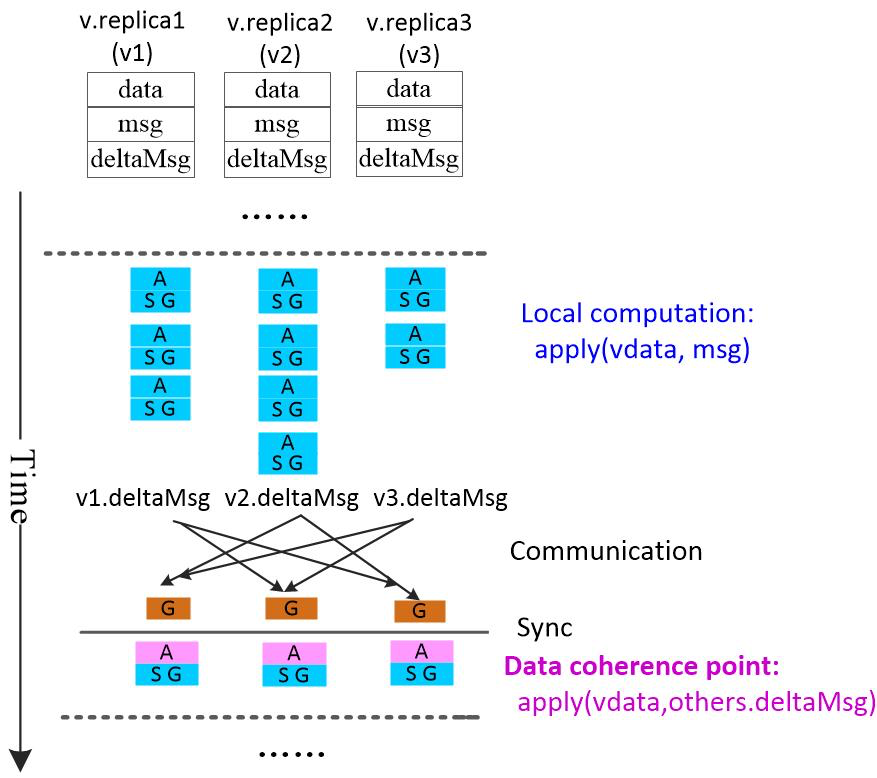
\includegraphics[height=12cm]{lazy_data_coherency.png}
\bicaption{点$v$的延迟数据一致性过程\cite{zlj2018}}{ lazy data coherency for replicas of v}
\label{fig:lazy_data_coherency}
\end{figure}

\subsection{延迟数据一致性方法的开启策略}
% 现有的开启策略,及不足之处

数据一致性节点的选择,也就是 延迟数据一致性方法(LazyAsync)的开启策略, 是 LazyAsync 的重要组成部分。
% 延迟数据一致性方法要解决的一个重要问题就是它的开启策略。
在把迭代公式修改为差值累加的形式之后, LazyAsync 方法正是通过lazy data coherency 的方法来减少冗余的通信和同步。
LazyAsync 的开启策略指的是系统应该在何时对副本点开启 lazy data coherency,
让各副本点独立计算数轮之后再进行消息交换,以及lazy data coherency 持续多久。
一种策略是立即进入策略,即系统一开始运行就启用 lazy data coherency。
另一种策略是手动调优策略,即不断的手动指定启用 lazy data coherency 的全局超步迭代轮次,
然后取其中性能提升最好的一个结果。
手动调优策略虽然不实用但是能够得出LazyAsync在指定算法和输入图上的相对最优的性能提升效果。
在实验中我们发现,随着这些具体策略的不同,系统得到的加速比也不同。
在有些算法和输入图上立即进入策略就能得到相对最好的性能提升效果,
在有些算法和输入图上需要手动调优才能得到相对最好的性能提升效果。
显然这个策略既不是越早越好,也不是越晚越好,过早开启或者过完开启都有可能得不到相对最优的性能提升。

在之前的工作中,我们采用了一个Input-behavior-interval决策树模型来作为LazyAsync的开启策略。
如图\ref{fig:dtree}所示,这个决策树模型采用两个特征作为判断条件:

\begin{enumerate}
  \item 输入图的本地性(locality)。我们使用边和顶点的比例 $\frac{E}{V}$ 和复制因子 $\lambda$ 来表示输入图的本地性。
  其中,复制因子 $\lambda$ 定义为整个图中所有顶点的平均副本点数,也就是总的副本点数于总的顶点数的比值。
  \item 图算法的运行时特征。大多数图算法都是迭代式地进行计算,不断地更新顶点的数据直至达到某个特定的收敛条件。
  在每一轮的迭代中,顶点的活跃点数\verb|vcnt| 是不断变化的。
  我们使用活跃顶点数的变化趋势来描述算法的特征。
  具体的,用如下公式进行计算:
  \begin{equation}
  \label{equ:chap04:trend}
  trend = \frac{vcnt^{t-1}-vcnt^t}{vcnt^{t-1}}
  \end{equation}
  我们在数据一致性阶段计算每一轮迭代时的活跃顶点数的下降趋势 \verb|trend|,如果 \verb|trend| 是负值,那么算法处于一个上升阶段,否则,则处于下降阶段。
\end{enumerate}

\begin{figure}[!htbp]
\centering
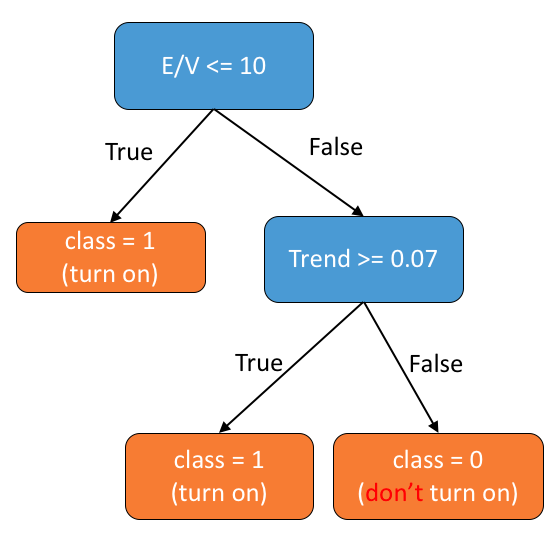
\includegraphics[width=0.40\textwidth]{decision_tree}
\bicaption{决策树模型\cite{zlj2018}}{Dceieson Tree Model}
\label{fig:dtree}
\end{figure}


Input-behavior-interval 决策树模型是一个离线调优模型。
它的基本思路是先通过手动调优找到各种情况组合下的相对最优的LazyAsync的开启策略。
然后对这个过程中产生的大量数据集进行训练拟合。
最后把拟合得到的决策树模型反代入到系统实现中作为一个在线的判断策略。


Input-behavior-interval 决策树模型并不能真正有效地解决 LazyAsync 的开启策略问题。
一方面在 Input-behavior-interval 决策树模型的训练过程中需要手动选择各种特征点组合进行试错。
另一方为了得到训练数量数据,也需要事先在大量的算法和输入图组合上进行繁琐的手动调优。
最重要的是基于机器学习方法得到的优化方法存着固有的过拟合或泛化能力不足的问题。
实际的计算过程中如果遇到训练集和验证集中没有遇到过的例子,决策树模型指导下的LazyAsync可能无法得到相对最优的性能提升。
图\ref{fig:dtfail}就给出了这样一个例子。
图\ref{fig:dtfail}对比了在不同集群配置环境下,同一算法分别采用基于eager data coherency的同步引擎,
基于决策树开启策略的LazyAsync,基于手动调优策略的LazyAsync三种方法进行计算所用的运行时间。
从图中可以看到在8机,24机,48机的集群环境中,决策树策略的运行时间和手动调优相一致,
可是在16机,32机,40机的集群环境中,决策树策略的运行时间与同步引擎的运行时间一致甚至更长。
也就是说在16机,32机,40机的集群环境中,决策树模型指导下的LazyAsync没有得到性能提升,出现了失灵的情况。

\begin{figure}[!htbp]
\centering
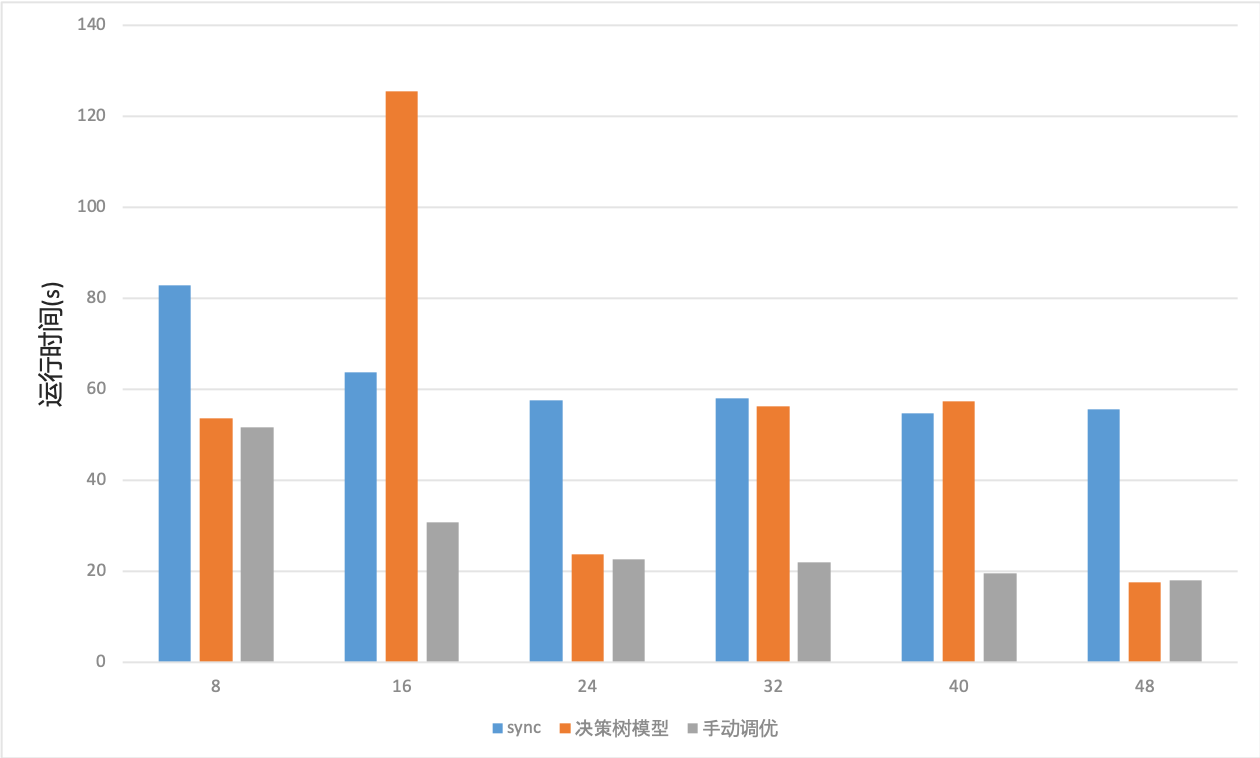
\includegraphics[width=0.40\textwidth]{dtreefail}
\bicaption{决策树失灵的情况}{Failure of decision tree}
\label{fig:dtfail}
\end{figure}

LazyAsync对副本上的数据进行lazy data coherency,
已经被证明为是一种行之有效的提升图计算执行效率的方法。
但是关于这种方法如何得到相对最优的性能提升这一问题还有待研究。
我们之前的工作中采用决策树的方法来解决 LazyAsync 的优化问题,
但是决策树模型一方面自身的训练需要一个繁琐的手动调优过程,另一方面也存在着失灵的情况,
因此并不能真正有效的解决这一问题。


自 Pregel 之后,研究者们使用各种优化手段提出了众多的分布式图计算框架。
这些框架大多数都对同一个顶点的不同副本点采取 eager data coherency 的方式。
在相关工作中,Hieroglyph\cite{ju2017hieroglyph}也同样使得同一顶点的不同的副本点可以独立本地更新自己的数据。
但是,Hieroglyph 关注于将计算从通信中解耦出来, 以获得充足的本地计算,并且需要用户定义模块来解决数据一致性的问题。
而 LazyAsync 则关注于延迟副本点间的数据一致性, 并同时减少全局同步 次数和网络通信,并且在编程框架内部自动地维护副本点之间的数据一致性。 
因此现有的研究不能直接用于处理我们提出的LazyAsync中遗留的优化问题。


本文通过进一步的实验,提出了一种基于解的局部性的自适应优化方法有效地解决了 LazyAsync 方法的优化问题。
本文先是通过实验和理论分析,解释了LazyAsync 方法在不同的开启策略下得到不同程度的性能提升的现象。
并从有效计算的角度出发,论证了 LazyAsync 在避免了 eager data coherency 的冗余通信和同步的同时,
自身却有可能带来一定程度的冗余计算,因而无法得到相对最优的性能提升。

通过分析全局解和局部解的关系,我们进一步发现了图计算过程中解的局部性规律。
解的局部性规律可以用于指导LazyAsync减少冗余计算。
基于这个规律,本文最终提出了一种基于解的局部性的在线自适应优化方法。
这种方法不需要事先的离线训练,同时也能正确处理决策树模型失灵的情况,因而有效地解决了
LazyAsync 方法的优化问题。



\chapter{LazyAsync 性能提升规律研究}
在前面的章节中我们提到LazyAsync遗留的主要问题是如何找到合适的开启策略从而得到相对最优的性能提升。
为此,本章对不同开启策略下得到不同程度的性能提升这一问题进行了研究,并通过实验得到了结论:
性能提升主要受冗余计算影响,不同开启策略下存在不同程度的冗余计算,冗余计算程度较低的开启策略能够获得更好的性能提升。
通过这一结论,本文对LazyAsync的性能提升的规律有了更深刻的认识。

本章将首先通过具体的例子对比基于eager data coherency 的同步引擎和基于 lazy data coherency 的LazyAsync来展示后者性能收益的来源,
然后再具体分析这个例子来说明LazyAsync中存在的冗余计算这一现象。
最后通过具体的实验数据论证正是冗余计算造成了不同开启策略下LazyAsync会得到不同程度的性能提升。



\section{冗余计算对 LazyAsync 的性能收益的影响}
\subsection{lazy data coherency 带来性能收益}
% \section{算法视角下的延迟数据一致性方法的性能收益来源}
% 为了解决LazyAsync的优化问题,本文首先对延迟数据一致性这种方法性能收益的来源进行了研究。
关于LazyAsync如何拿到性能收益,我们之前的工作其实已经有所解释。
之前的解释从分布式计算系统的角度阐述,把性能收益归因于全局超步迭代轮次和通信量的减少。
但是这种解释不足以说明这种方法为何有时性能收益较高有时却较低,以及为何有时全局超步迭代轮次减少计算时间却并没有明显减少。


本节继续从具体算法用例的角度来解释,LazyAsync 具体是减少了哪些部分的全局同步。
为此,本文以 单源最短路径算法(Single Source Shortest Path,SSSP)算法为例,在一个小图上分别以 基于 eager data coherency 的同步引擎
和 基于lazy data coherency的LazyAsync运行算法。
这样的对比直观地揭示出了从具体的算法角度而言,LazyAsync究竟是减少了哪些部分的全局同步。
同时,这里的对比过程也为后边的冗余计算问题的提出打下了基础。


为此,我们需要先对图计算中的 SSSP 算法进行介绍。
为了支持各种图算法,大规模图计算框架往往需要在底层图计算系统和上层具体的图算法之间进行抽象。
PowerGraph从单个顶点的角度出发\cite{McCune@CS15},把所有的图算法抽象为Gather,Apply,Scatter三个阶段。
用户使用框架提供的GAS编程接口可以实现各种图算法。
算法\ref{alg:SSSP}中描述了基于GAS编程接口实现的SSSP算法。
Gather阶段,提供了顶点访问周边邻居并拉取信息的接口,SSSP中不需要这个过程。
Apply阶段,提供了根据收到的消息及拉取到的信息,修改顶点上的数据的接口,SSSP中每个顶点根据收到的信息更新自己到 source 的距离。
Scatter阶段,提供了顶点访问周边邻居并推送信息的接口,SSSP中,每个顶点根据自己更新的距离,判断是否进一步激活自己的邻居顶点。

\algnewcommand{\LeftComment}[1]{\Statex \(\triangleright\) #1}


\begin{algorithm}[!htbp]
  \small
  \caption{基于GAS接口实现的 SSSP 算法\cite{low2013graphlab}}\label{alg:SSSP}
  \begin{algorithmic}[1]
    \Procedure{SSSP}{G(V,E,D)}
    \LeftComment{gather\_nbrs: empty}
    \State $gather(D_u,D_{(v,u)},D_v): return$     
    \State $sum(a,b) : return a\bigoplus b $ \Comment{\bigoplus \span : \span (min(a,b))}
    \State $apply(D_u, new\_dist): 
      \qquad D_u = new\_dist$
    \LeftComment{scatter\_nbrs: all\_out\_nbrs}
    \State $scatter(D_u, D_{(u,v)}, D_v):$     
    \If{ $ changed(D\_v) $ }
      \State { $ active(v, D_u+D_{(u,v)})$ }
    \EndIf
    \EndProcedure
  \end{algorithmic}
\end{algorithm}


\subsubsection{eager data coherency 中的SSSP算法}
下面以一个小图来具体说明 SSSP 在图计算框架中采用基于 eager data cohere- ncy 方法的同步引擎上的执行过程。
图\ref{fig:sssp-sync-iter}中展示了在一个小的输入图上,SSSP算法的执行过程。
这个小图由14个顶点和19条边构成,划分在3台机器上,以0号顶点为source,计算其他顶点到source的最短距离。
系统一开始会把消息值0发送给0号顶点,进而激活0号顶点,把0号顶点作为活跃点参与计算。

在第0轮迭代的apply阶段,0号顶点会根据收到的消息把自己顶点上的数据更新为0,
在第0轮迭代的scatter阶段,0号顶点的master部分和mirror部分会激活自己的本地邻居。
反映在图中就是,机器0上的master 0 激活了自己的本地邻居 master 1 和 mirror 11,
机器2上的mirror 0 激活了自己的本地邻居mirror 41 和 mirror 31。
这样,第0轮迭代后,0号顶点的1,11,31,41这4个邻居都被激活并发送了消息值1
(这里需要说明的是边上值缺省为1,所以发送了值1)。
消息发送完毕后第0轮迭代完成,系统进入第1轮迭代。

在进入第1轮的GAS实际计算之前,图计算的底层引擎会对系统中存在的消息进行收发处理,
把每一条消息送到其接收者master副本所在的机器上,并把接收者标记为新一轮的活跃点。
在消息处理完毕后,底层引擎会统计活跃点的数量,如果为0,那么迭代结束,运算完成,
如果不为0,那么继续进行GAS运算。
反映在图中,第1轮迭代,顶点1,11,31,41成为活跃点。
在第1轮迭代的apply阶段,机器0上的master 41,master 1根据收到的消息把自己顶点上的数据更新为1,
机器1上的master 11根据收到的消息把自己顶点上的数据更新为1,
机器2上的master 31根据收到的消息把自己顶点上的数据更新为1。
Apply阶段结束后,系统采用急切一致性的方法,把1,11,31,41号顶点master部分的信息立即同步到其他mirror顶点上去,
这样顶点的master部分和mirror部分就立即实现了一致性。
在scater阶段,1,11,31,41这4个活跃点的master部分和mirror部分都会执行scatter操作去激活自己的本地邻居。
反映到图中,
机器0上的mirror11会激活它的邻居master2,master 1则由于本地没有邻居不进一步激活,
机器1上的master 11也由于本地没有邻居不进一步激活,
机器2上的mirror 41则会激活本地邻居master 61,mirror 1则会激活本地邻居mirror 2。

这样这些被激活的2号顶点和61号顶点则会进一步作为第2轮的活跃点进行计算,直到最后系统中没有活跃点,运行结束。
最终在经过10轮迭代之后,图中的顶点都求得了到source的最短路,运算结束。


\begin{center}
  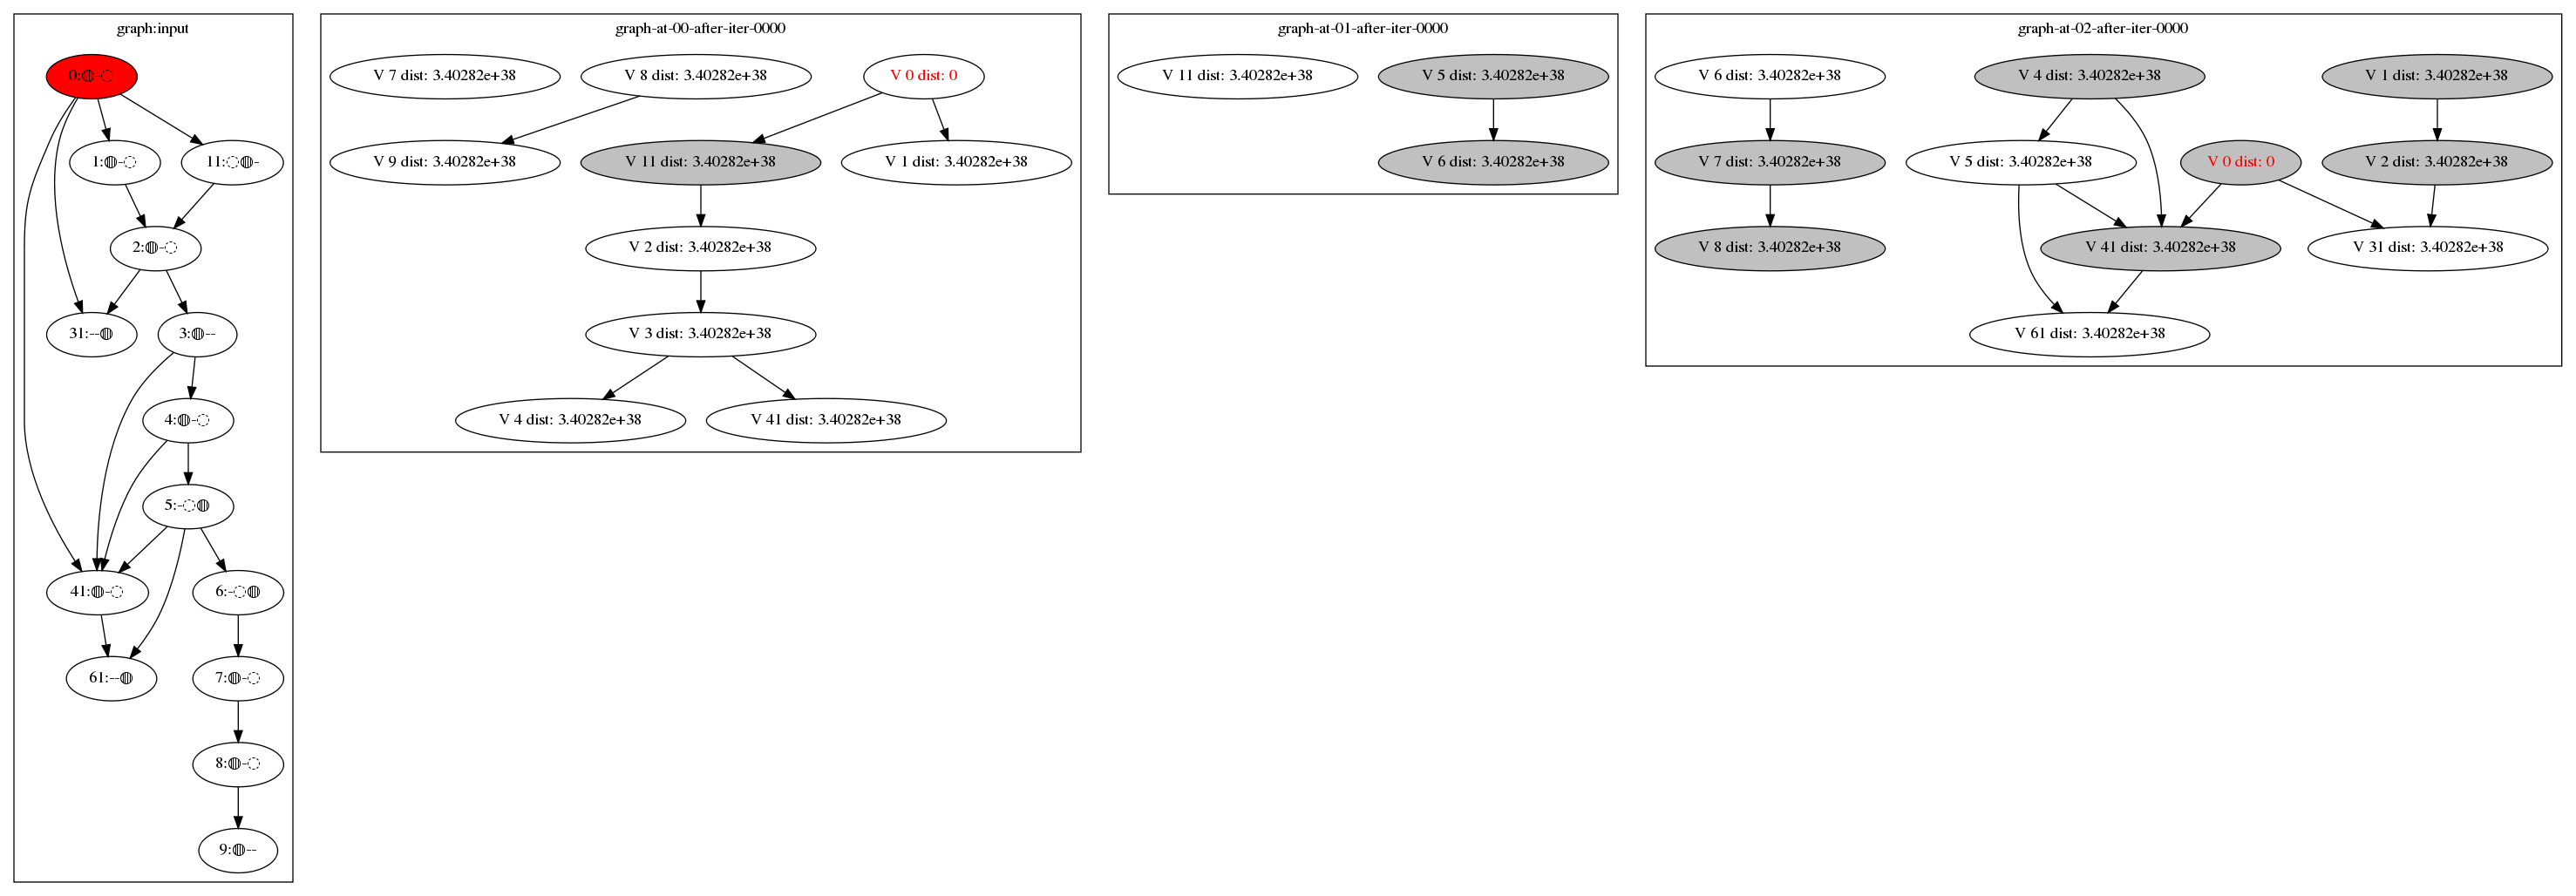
\includegraphics[width=0.8\textwidth]{sync-iter0.png}
  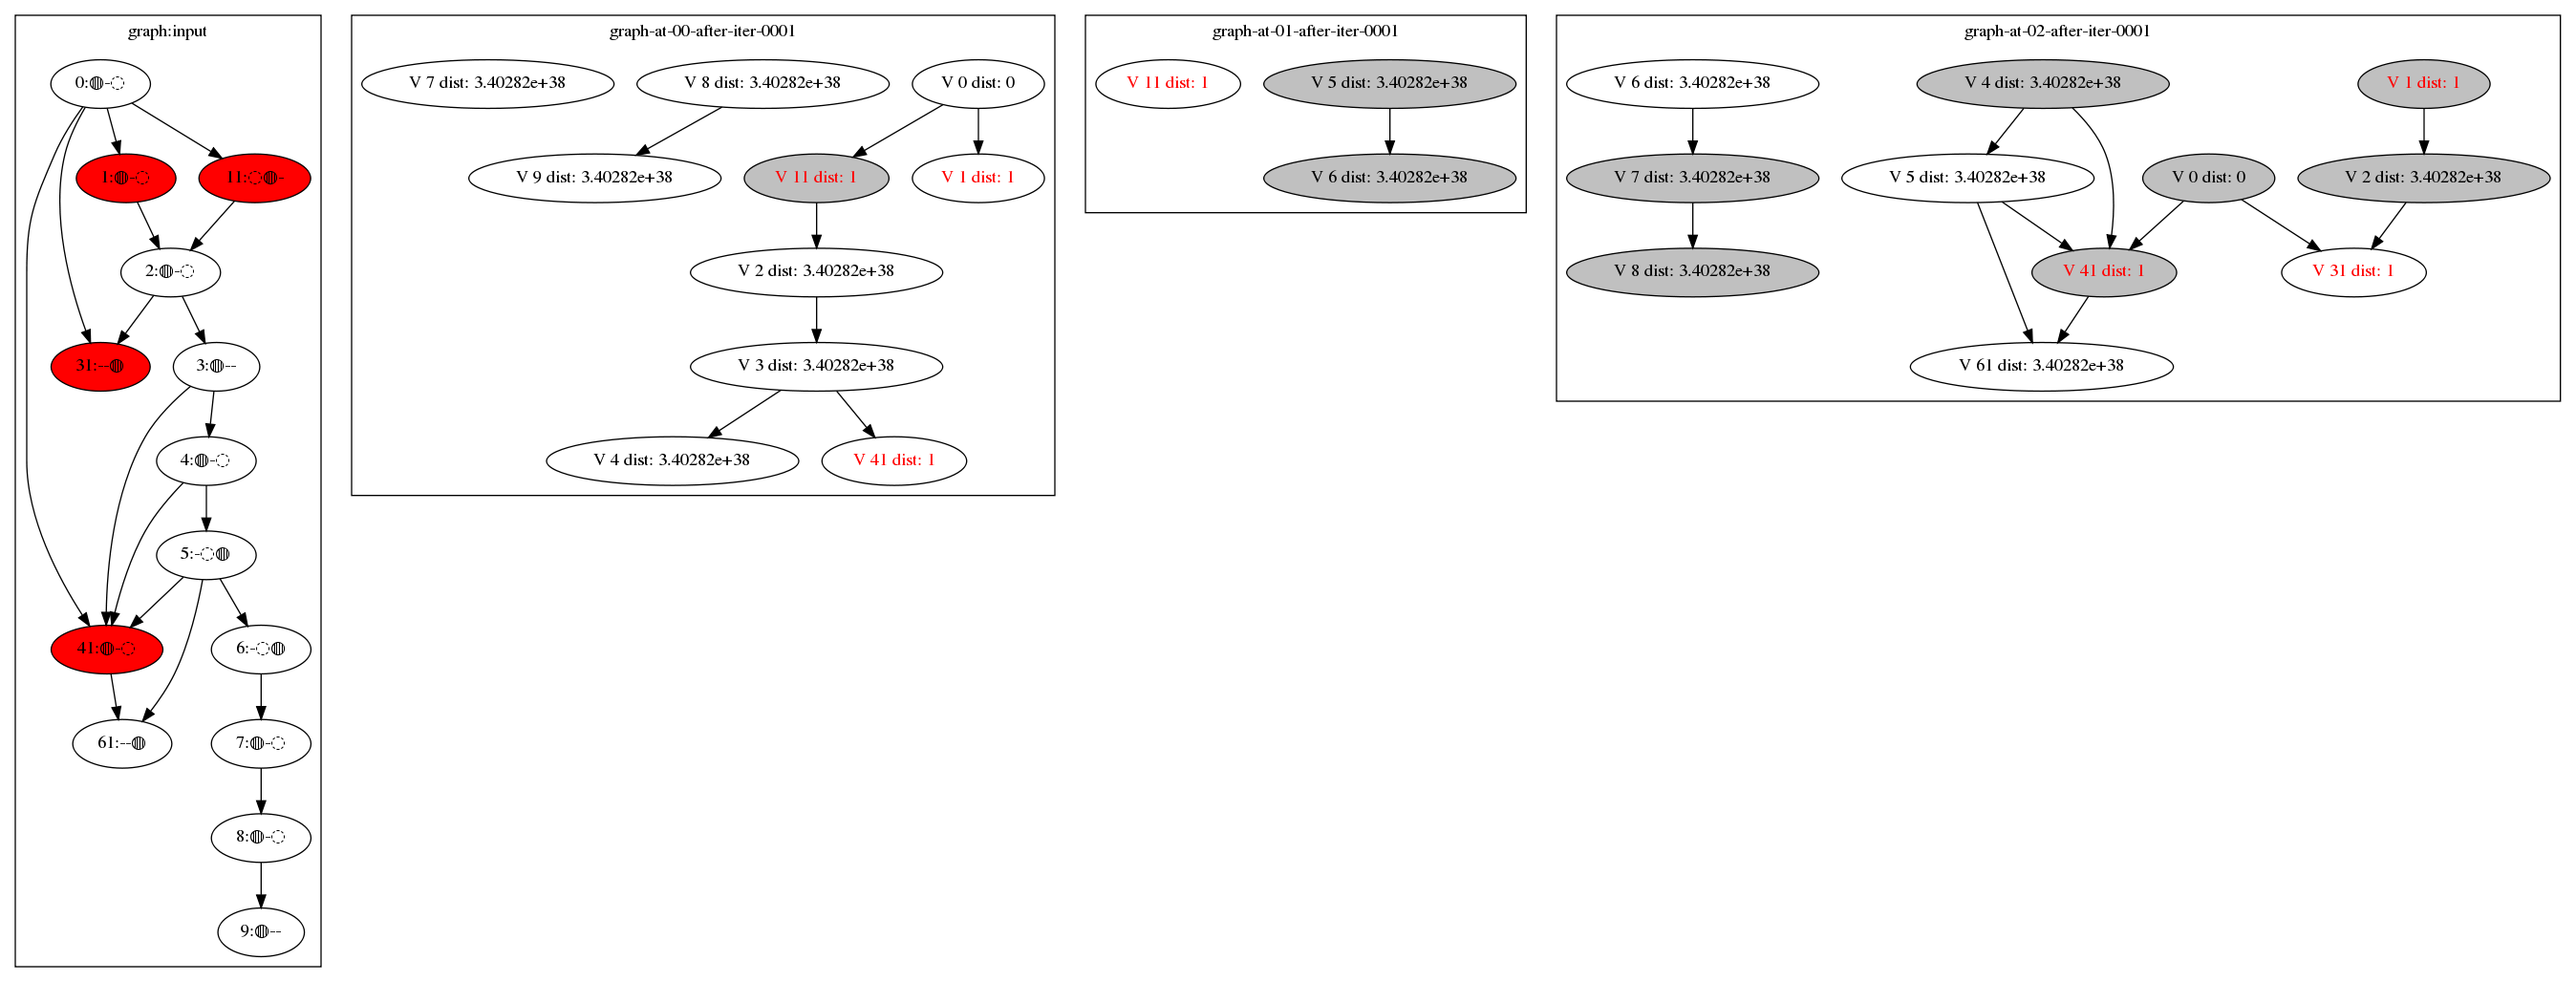
\includegraphics[width=0.8\textwidth]{sync-iter1.png}
  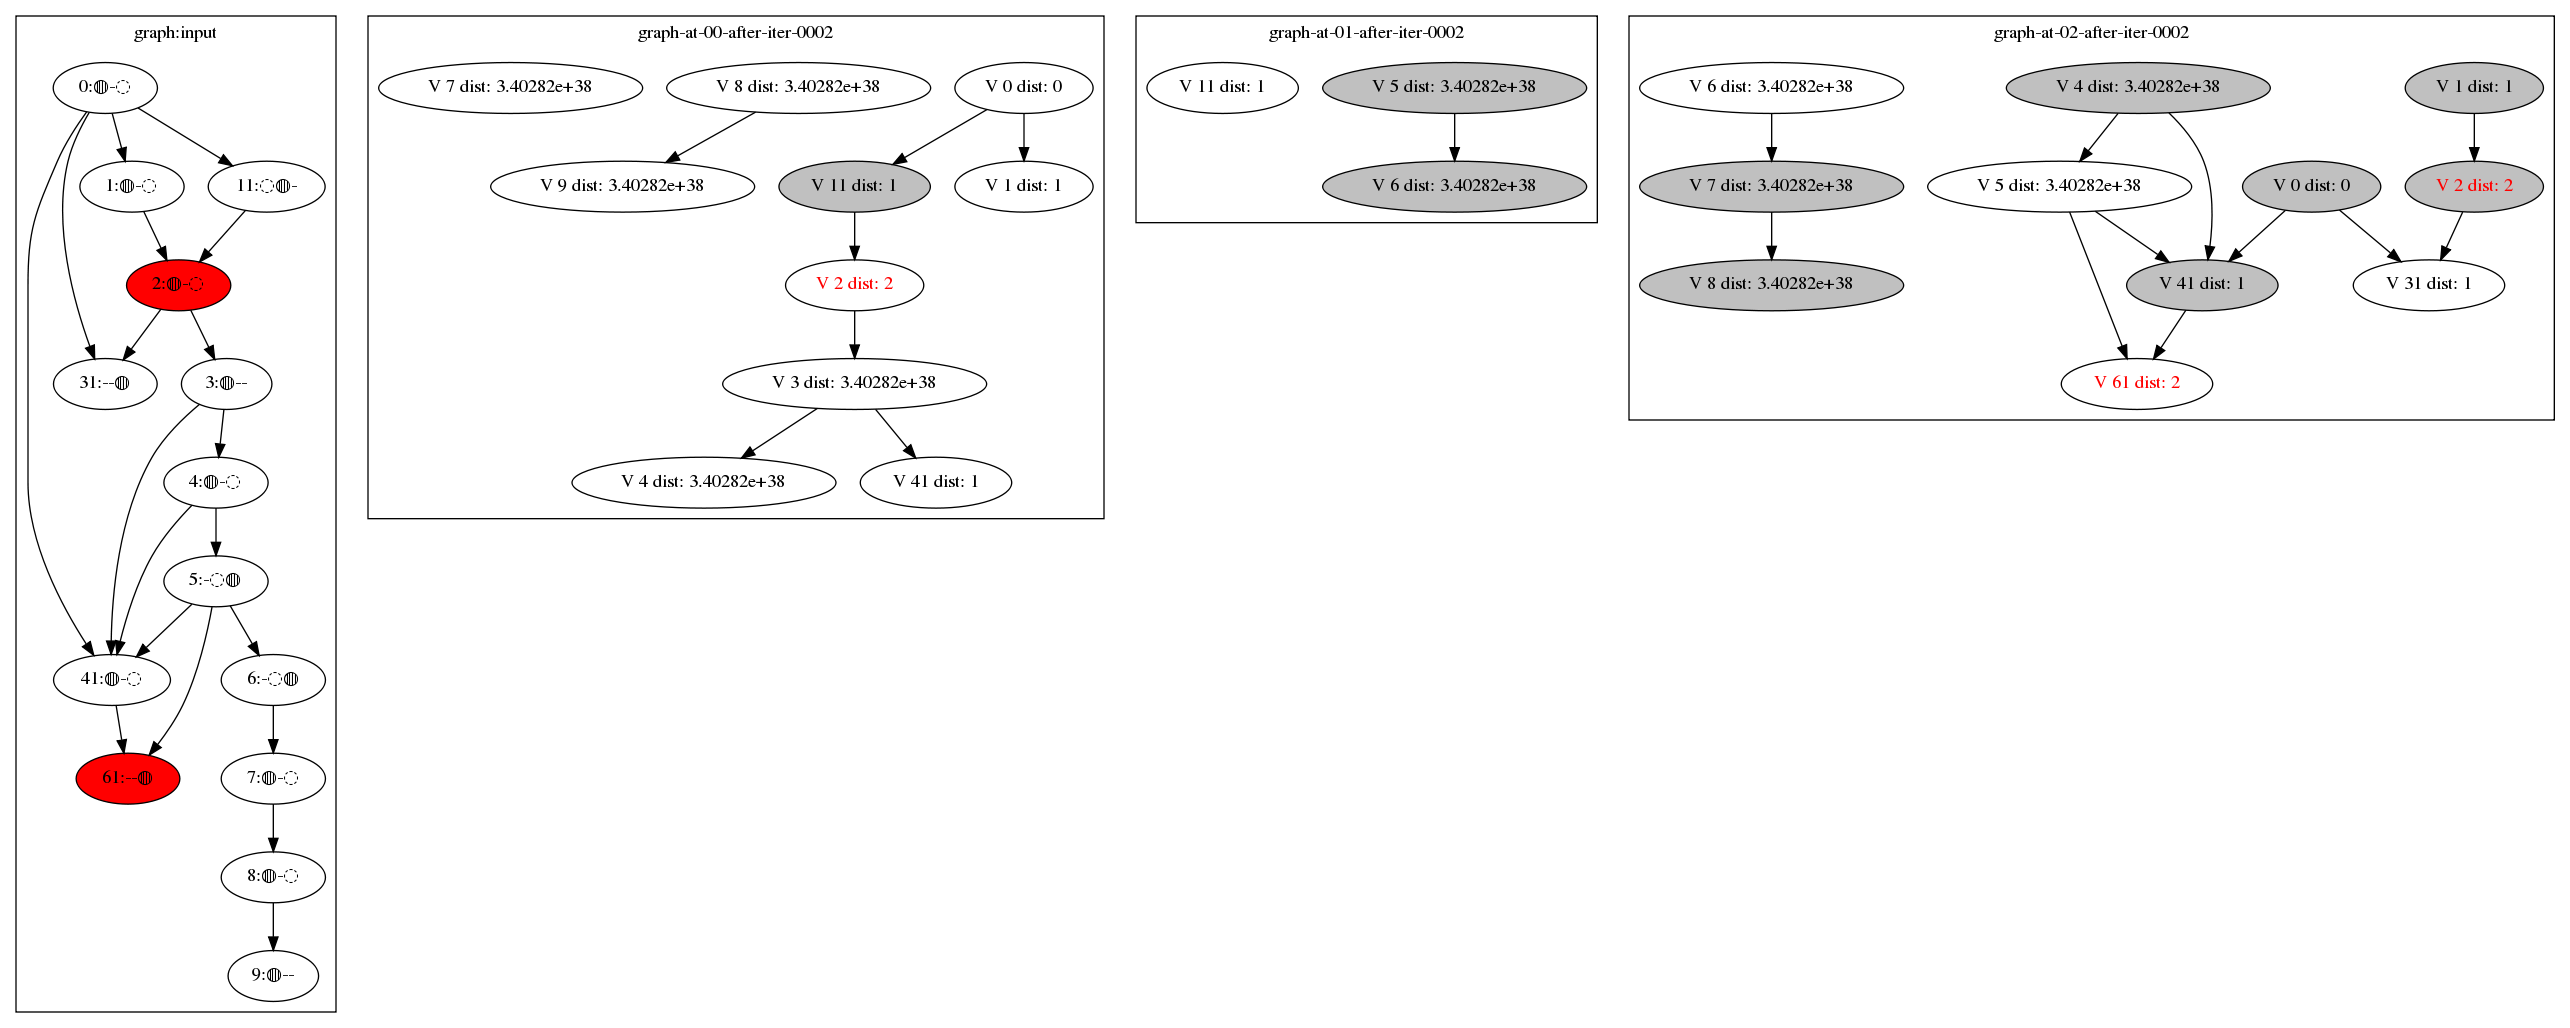
\includegraphics[width=0.8\textwidth]{sync-iter2.png}    
  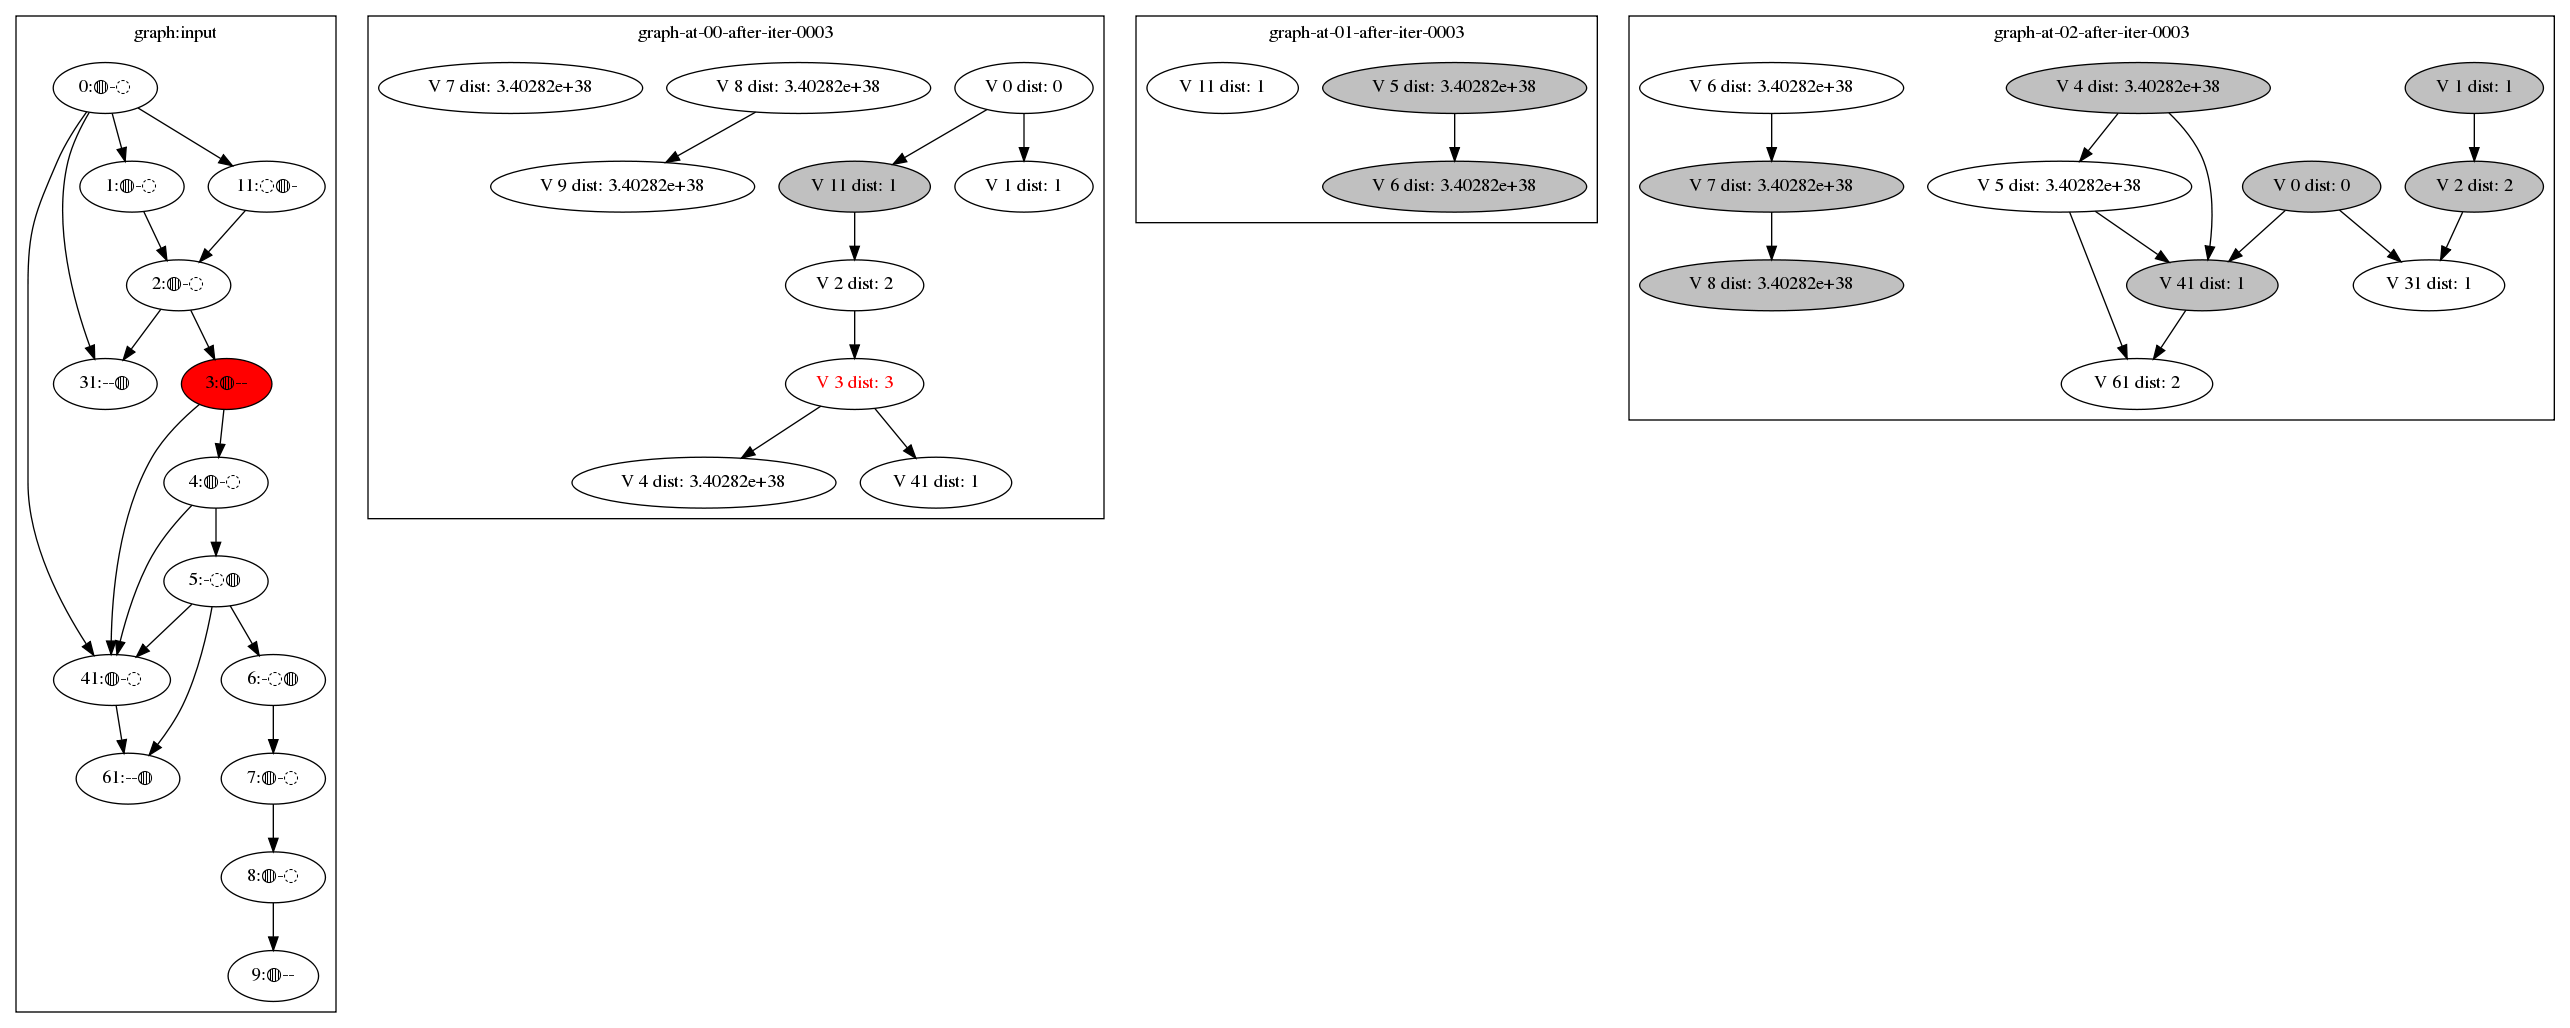
\includegraphics[width=0.8\textwidth]{sync-iter3.png}    
  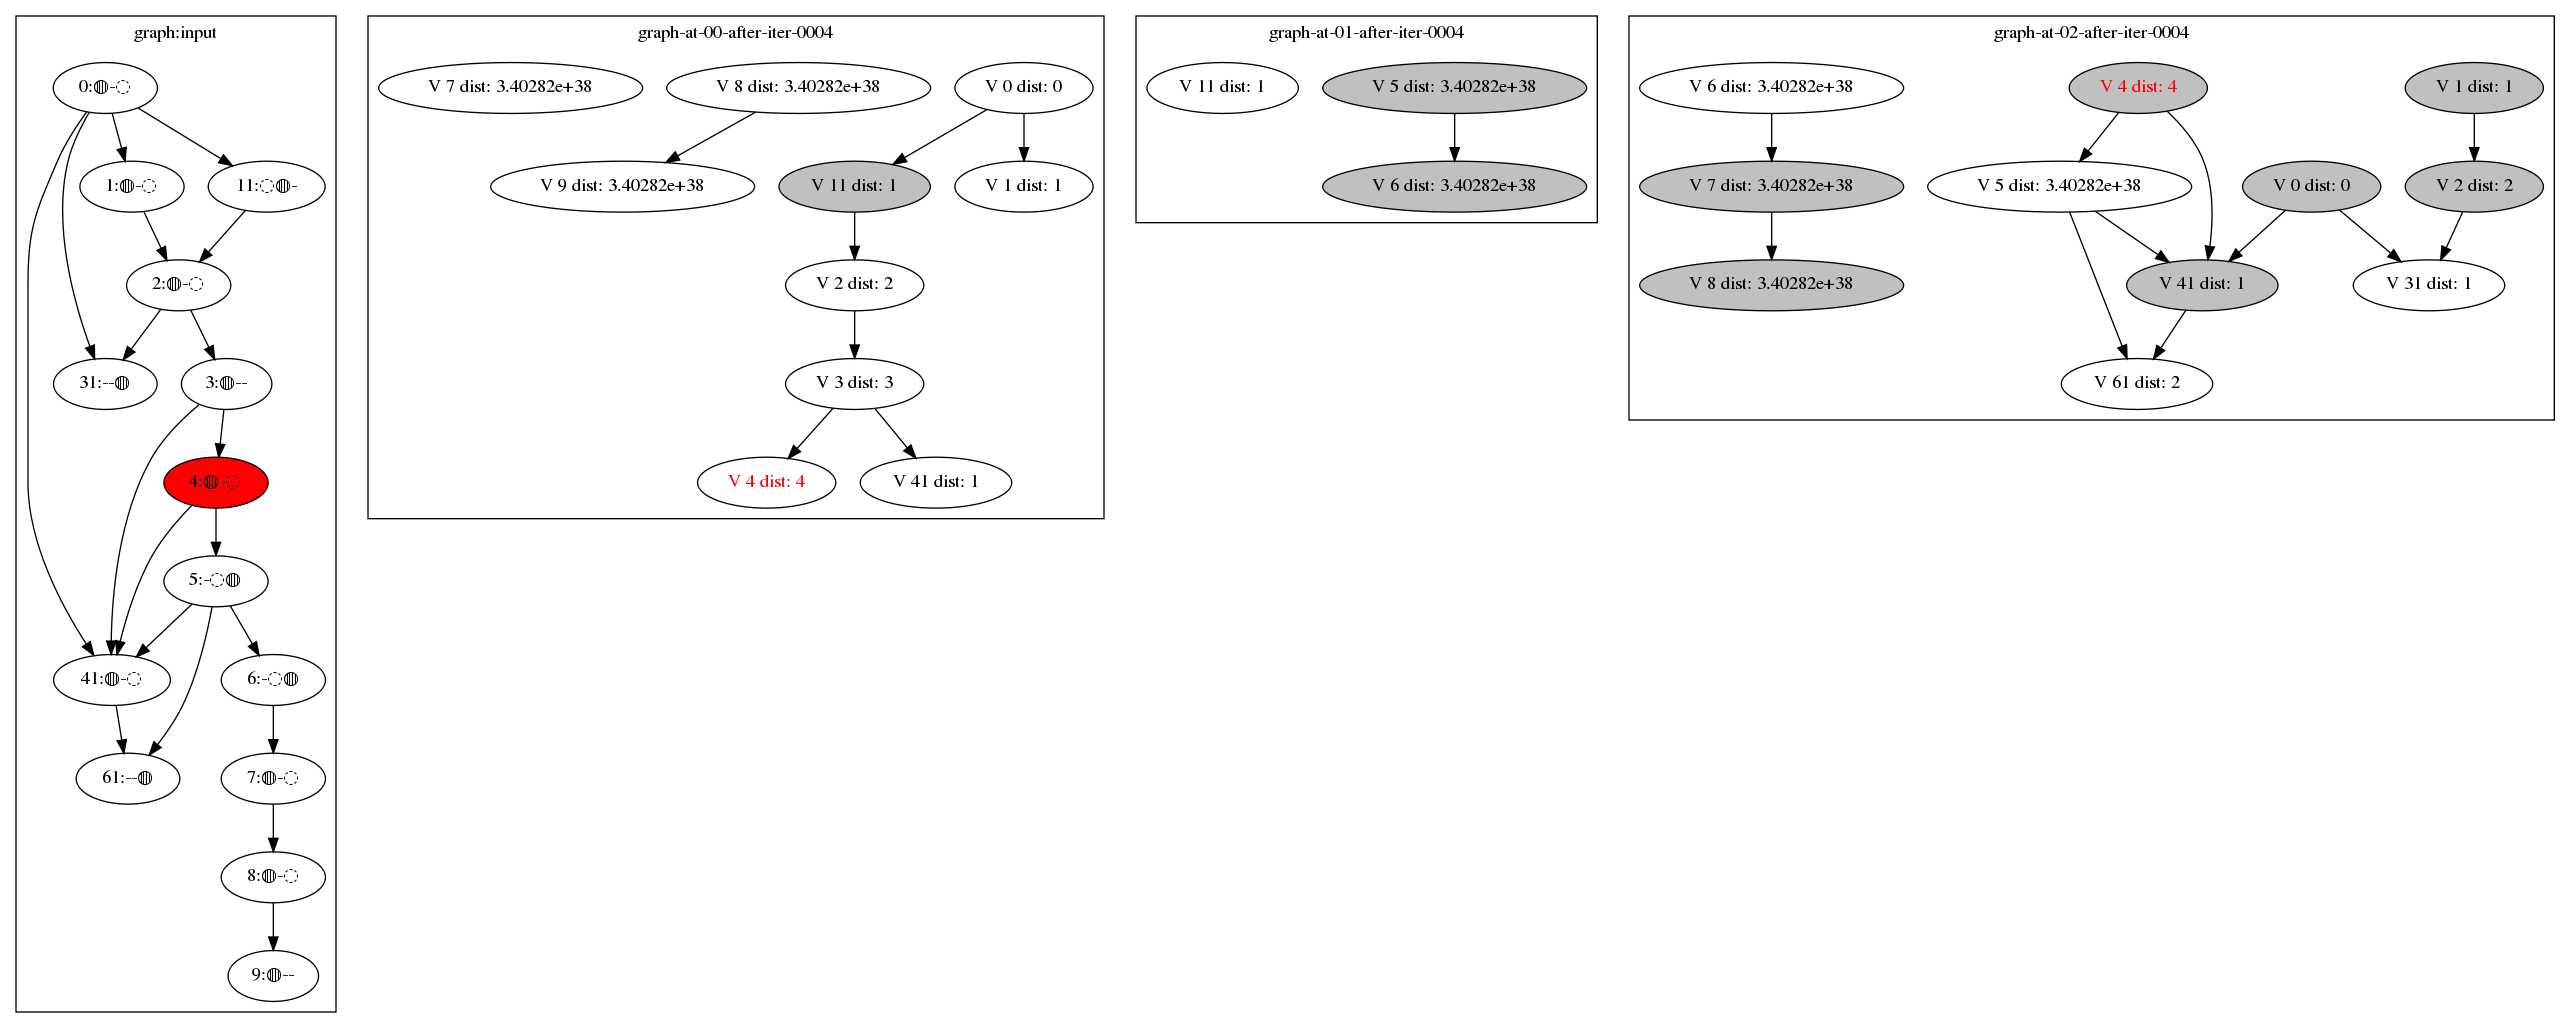
\includegraphics[width=0.8\textwidth]{sync-iter4.png}    
  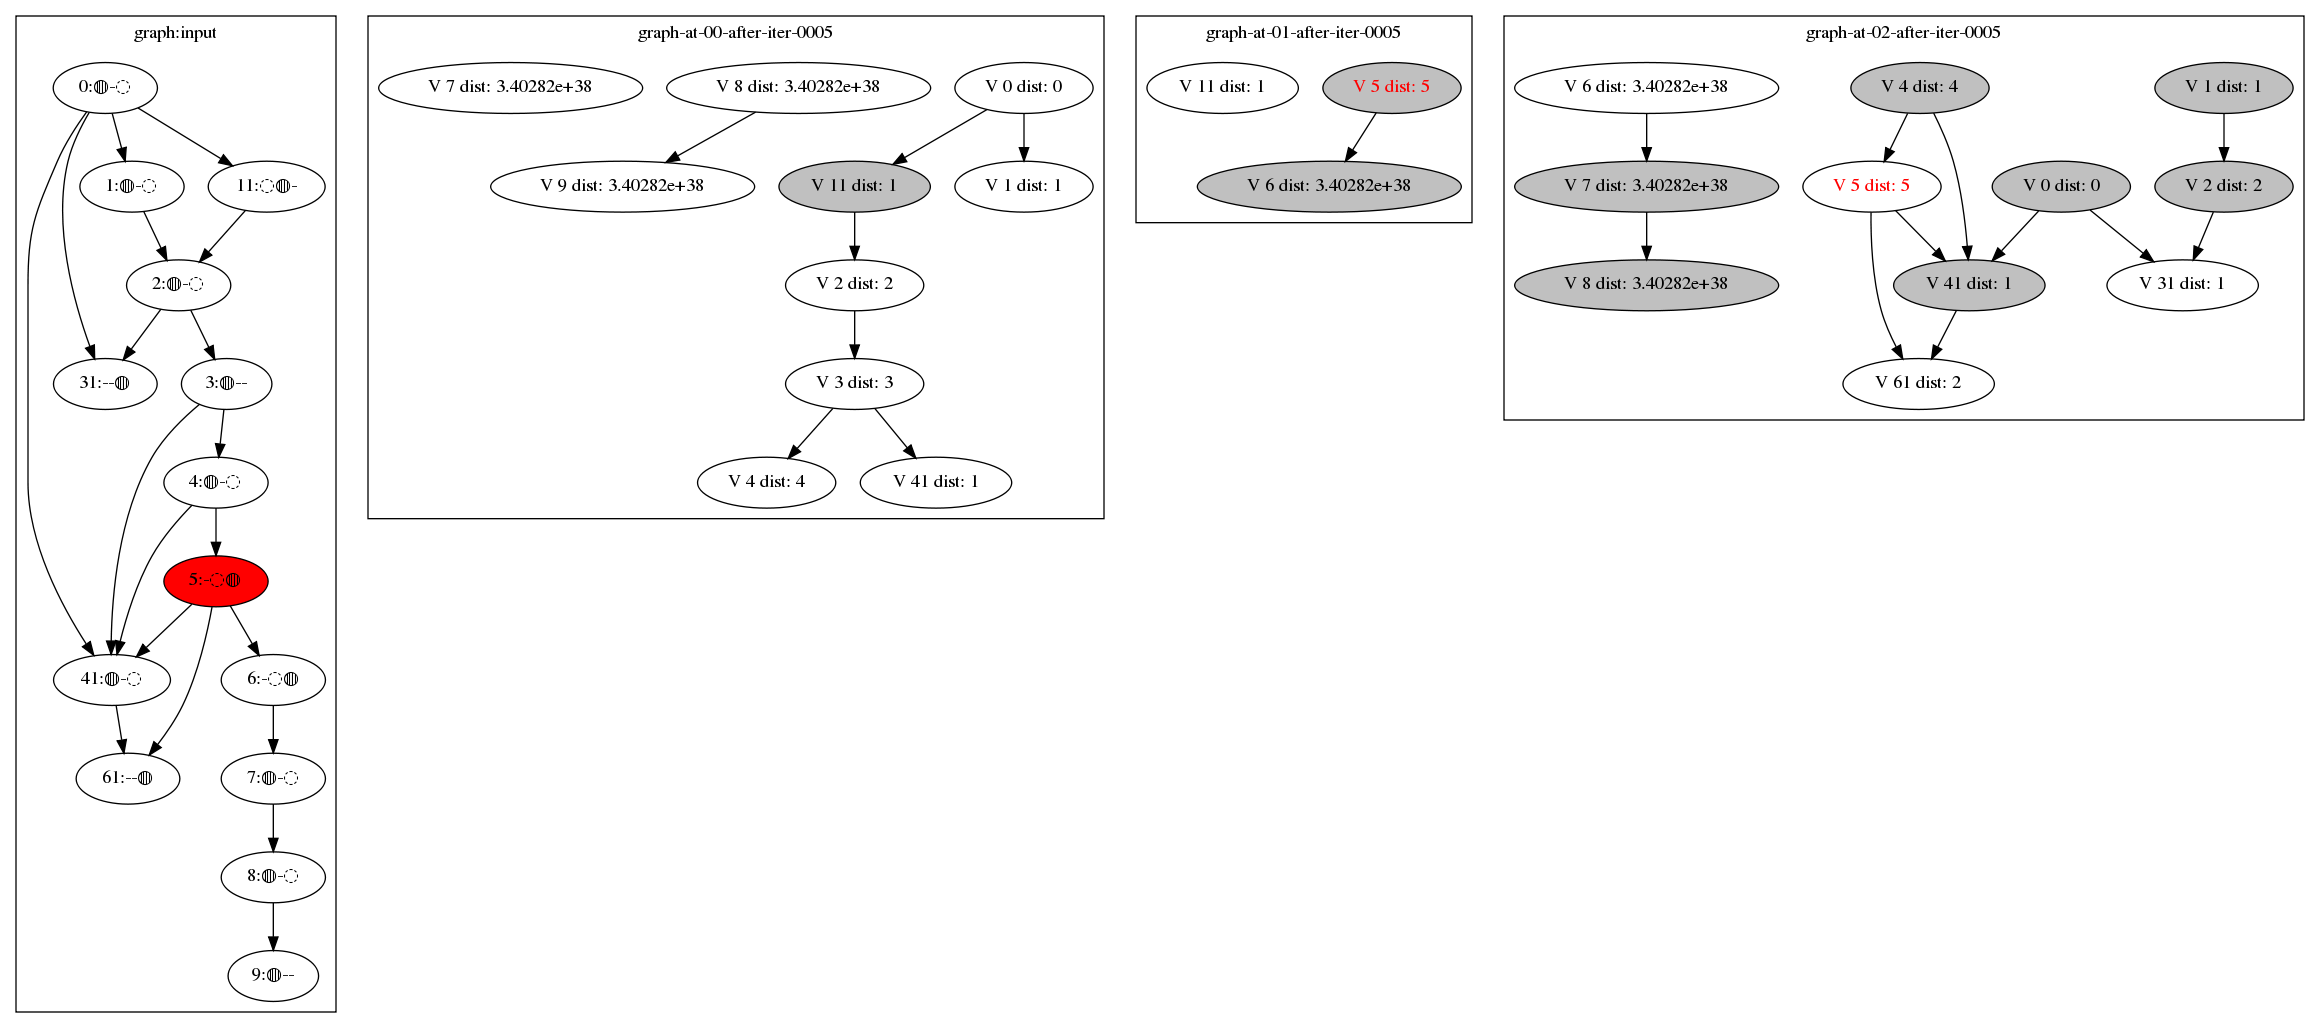
\includegraphics[width=0.8\textwidth]{sync-iter5.png}    

  \captionof{figure}{同步引擎中SSSP算法的迭代过程}
  \label{fig:sssp-sync-iter}
\end{center}  

\subsubsection{lazy data coherency 中的SSSP算法}

在基于lazy data coherency 的LazyAsync中,SSSP算法能够以更少的迭代次数得到同样的结果。
我们以同样的输入图来说明这一点,同时直观的展示LazyAsync的具体原理。

\begin{center}
  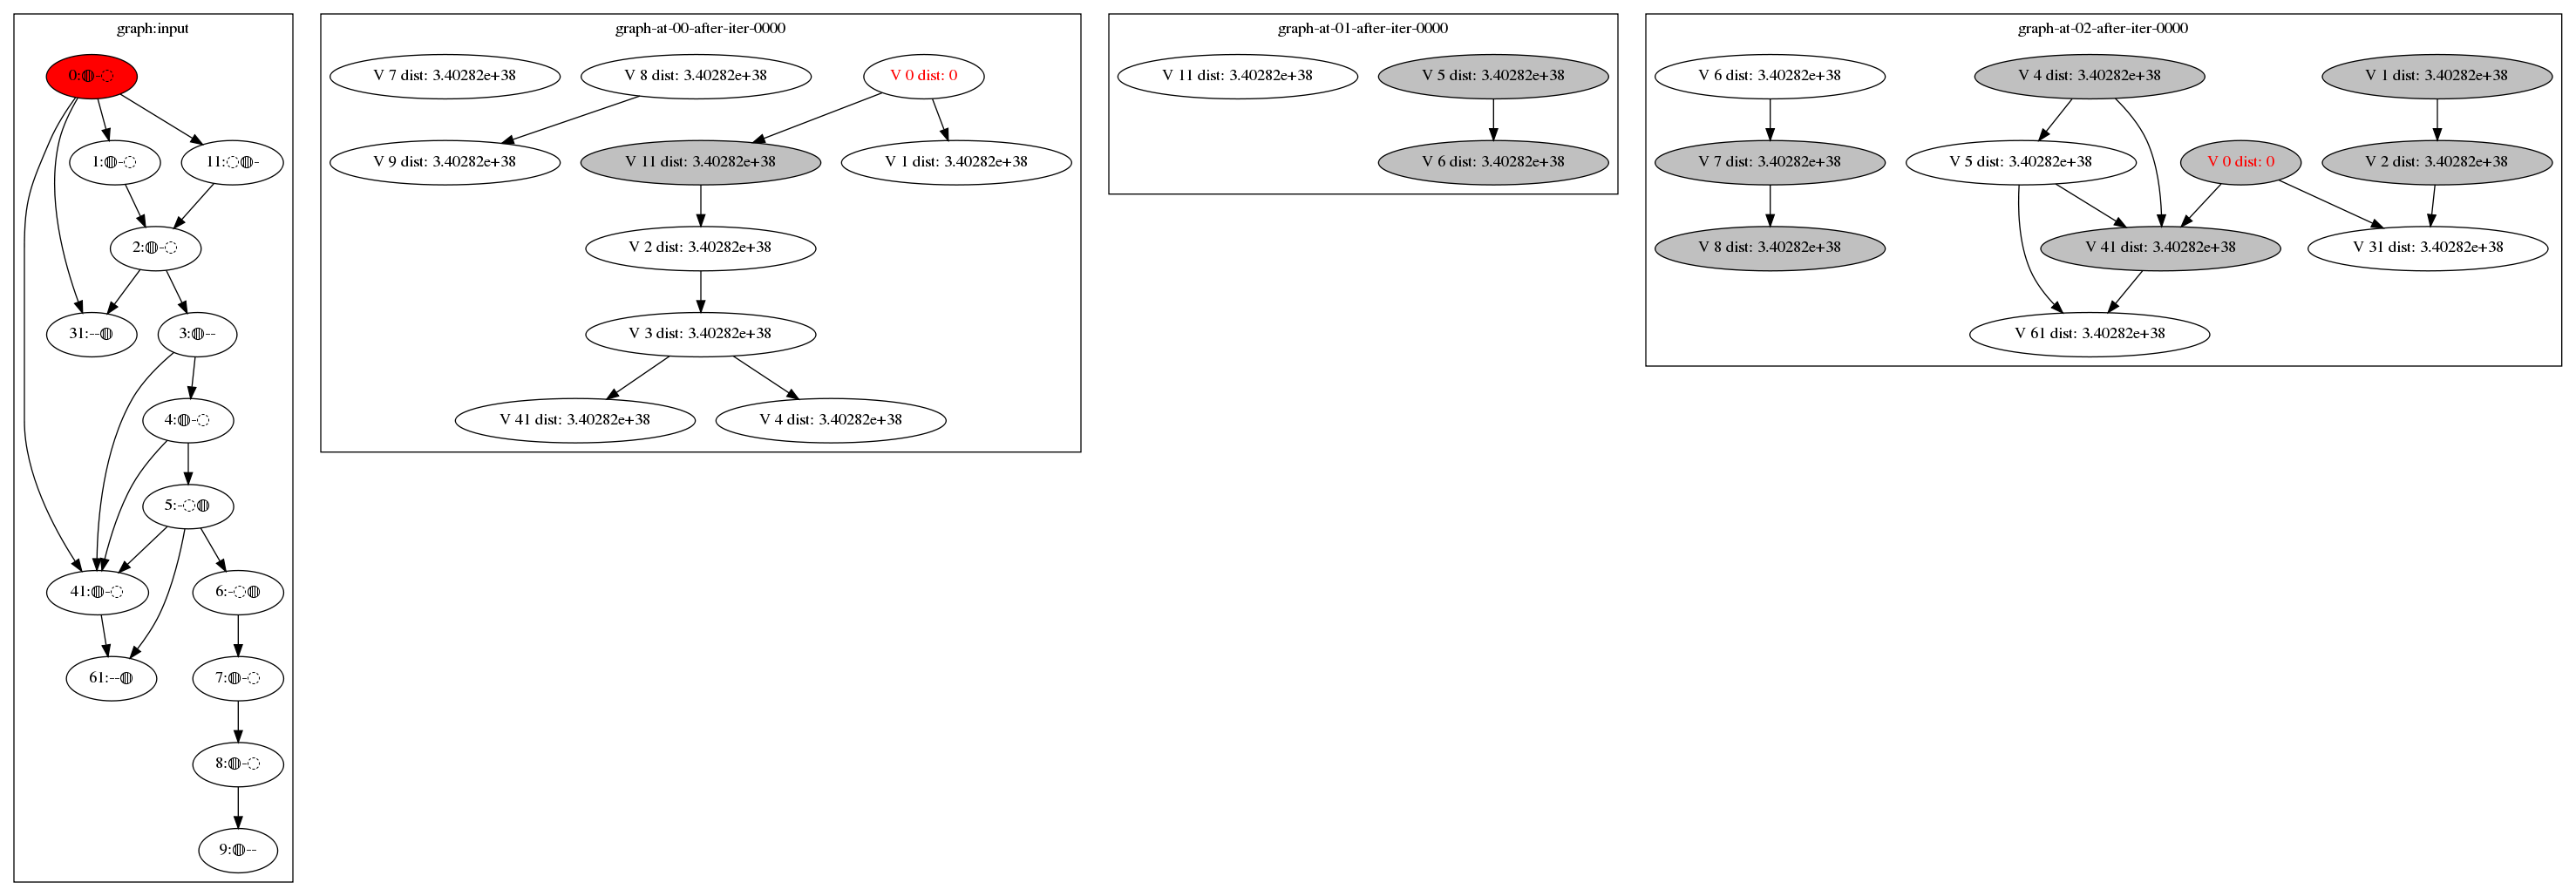
\includegraphics[width=0.8\textwidth]{lazy-iter0.png}
  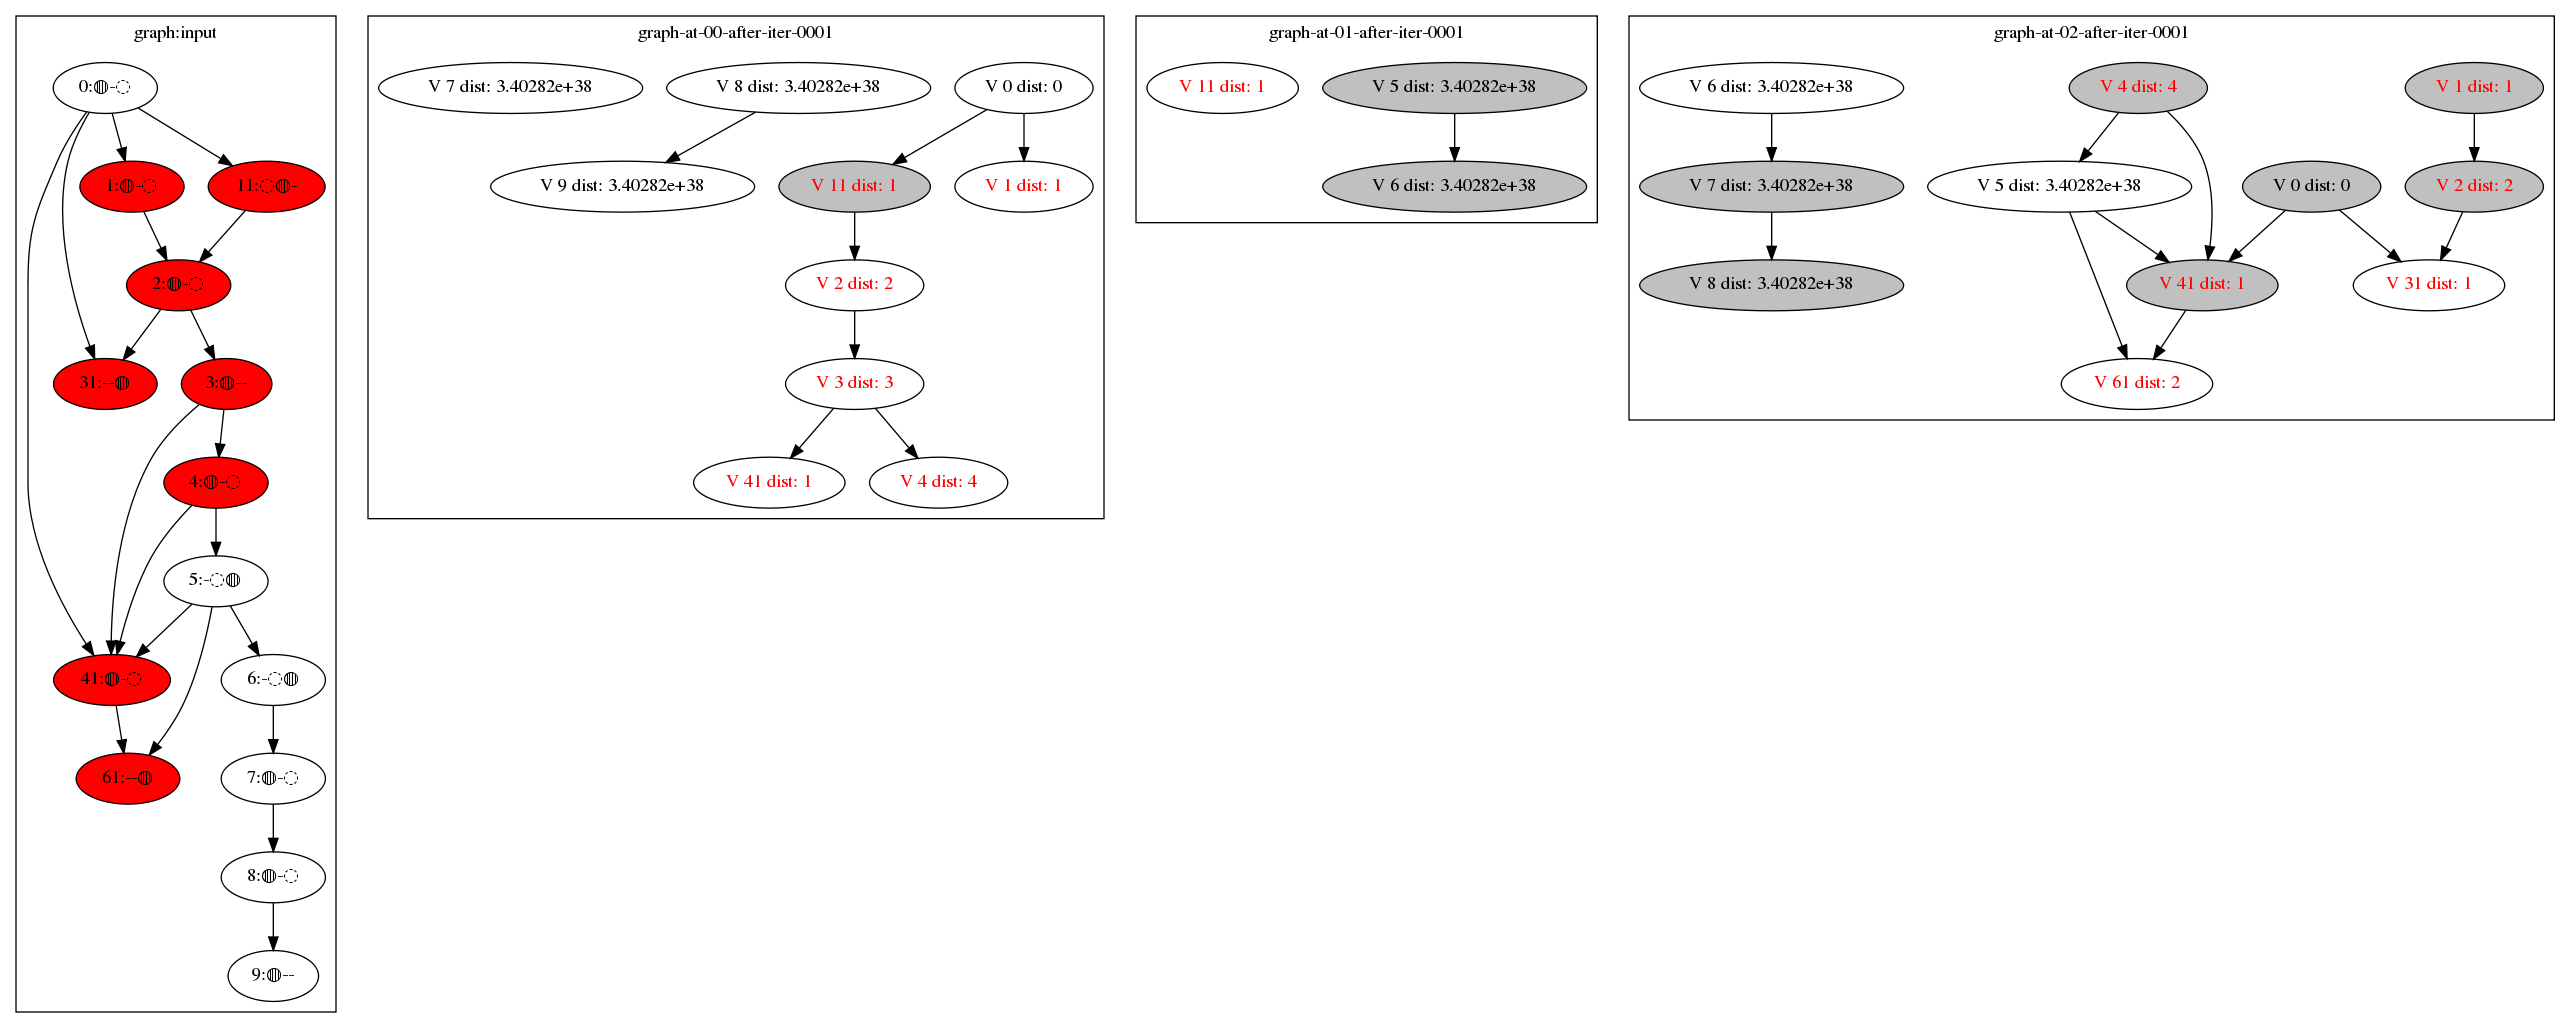
\includegraphics[width=0.8\textwidth]{lazy-iter1.png}
  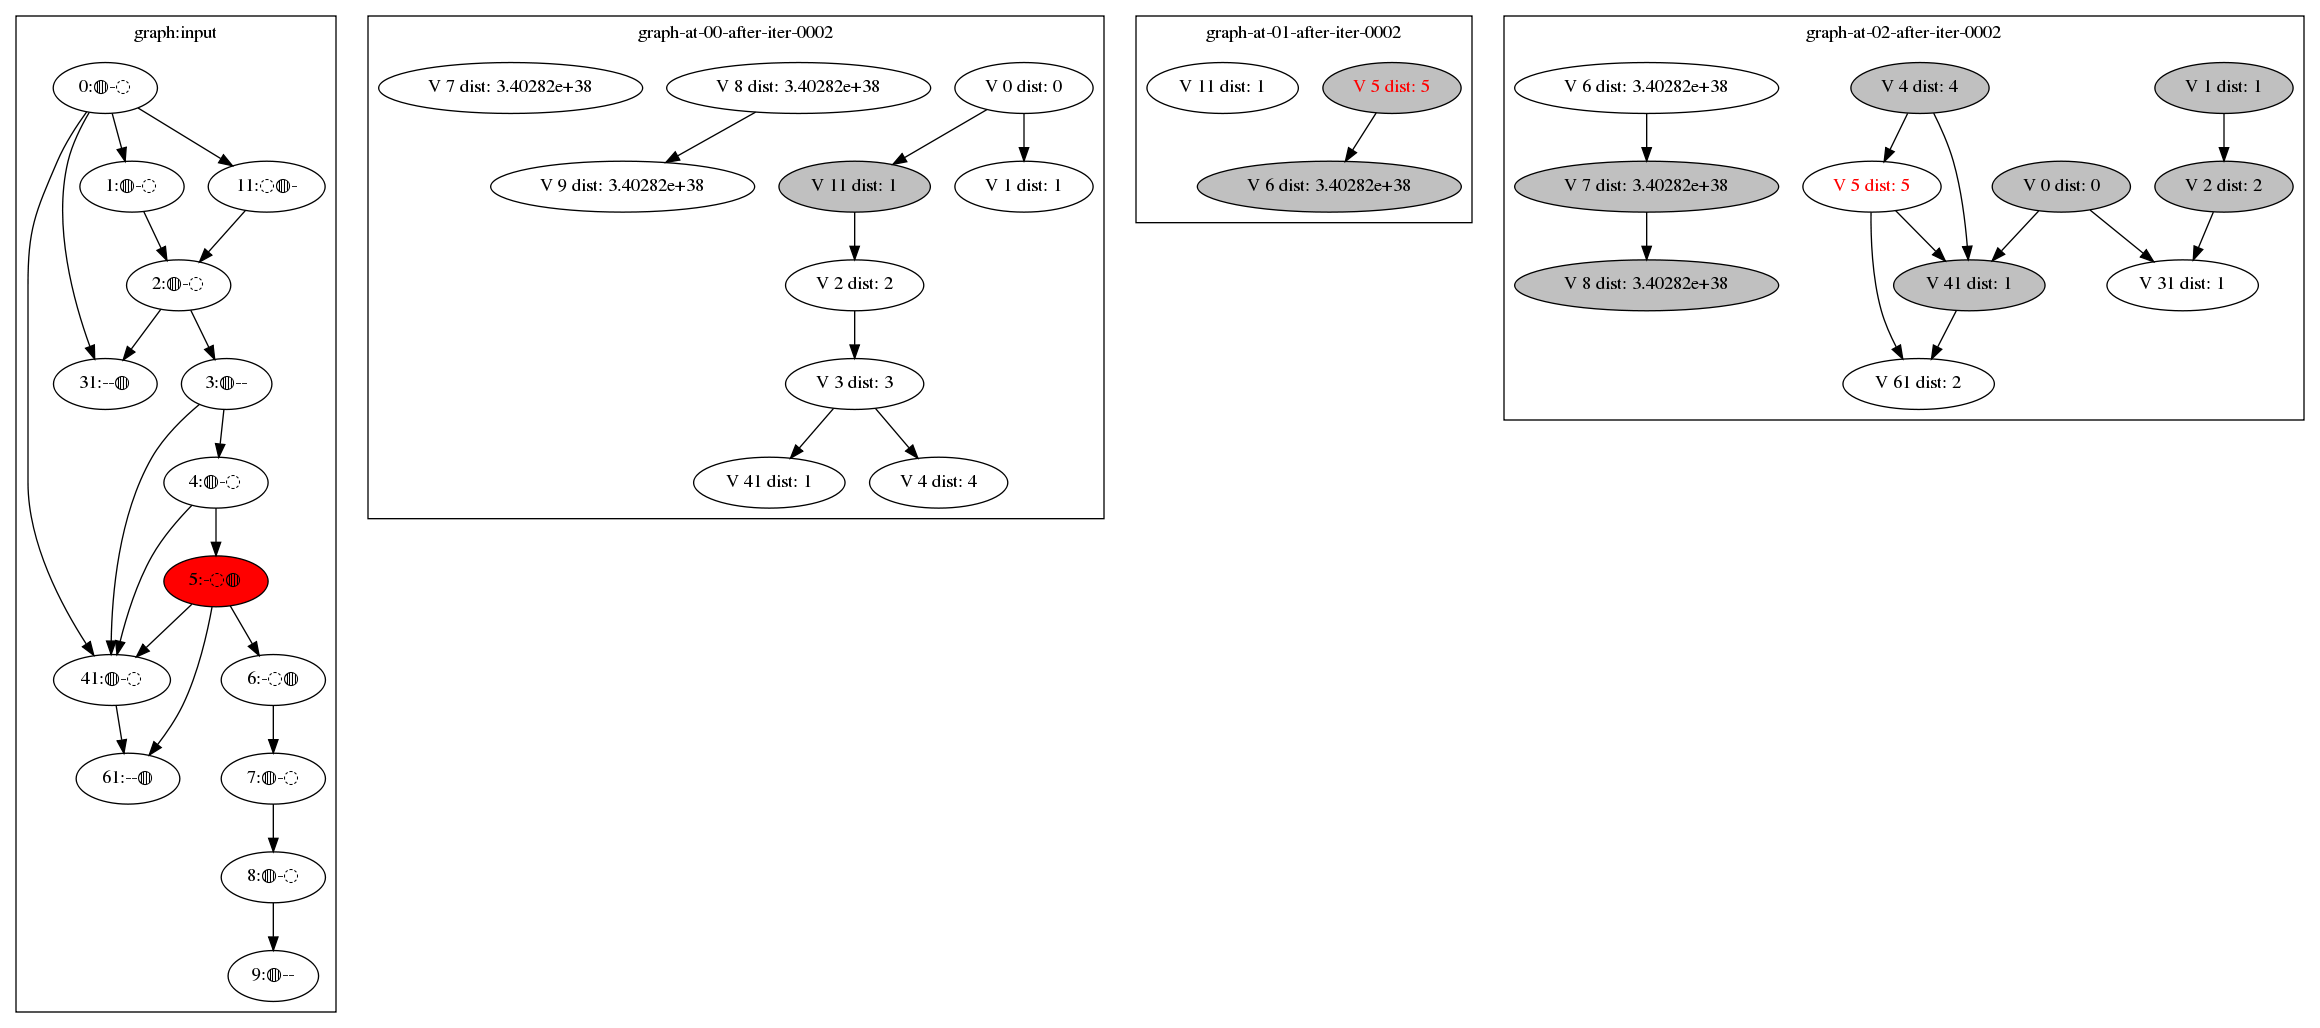
\includegraphics[width=0.8\textwidth]{lazy-iter2.png}    
  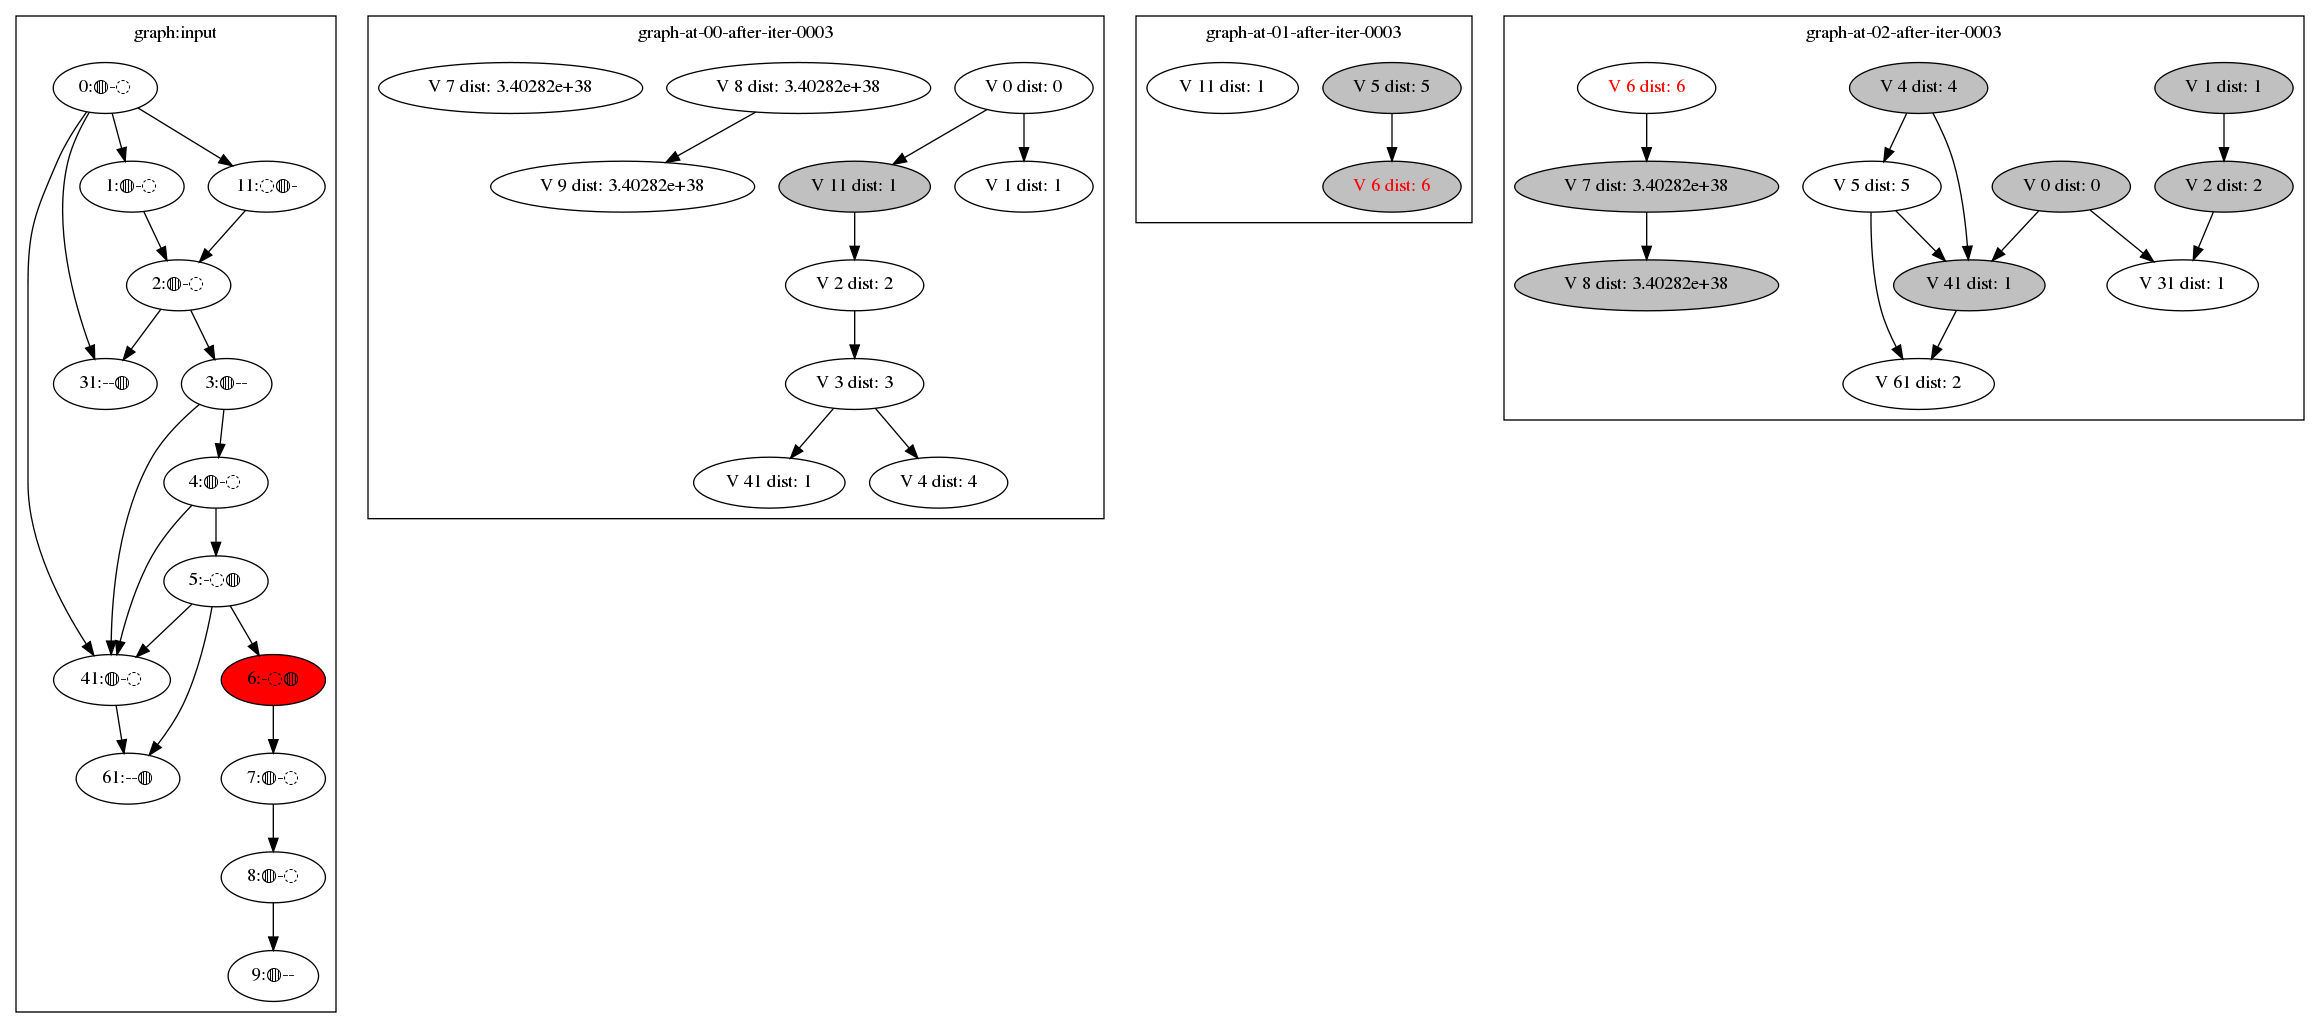
\includegraphics[width=0.8\textwidth]{lazy-iter3.png}    
  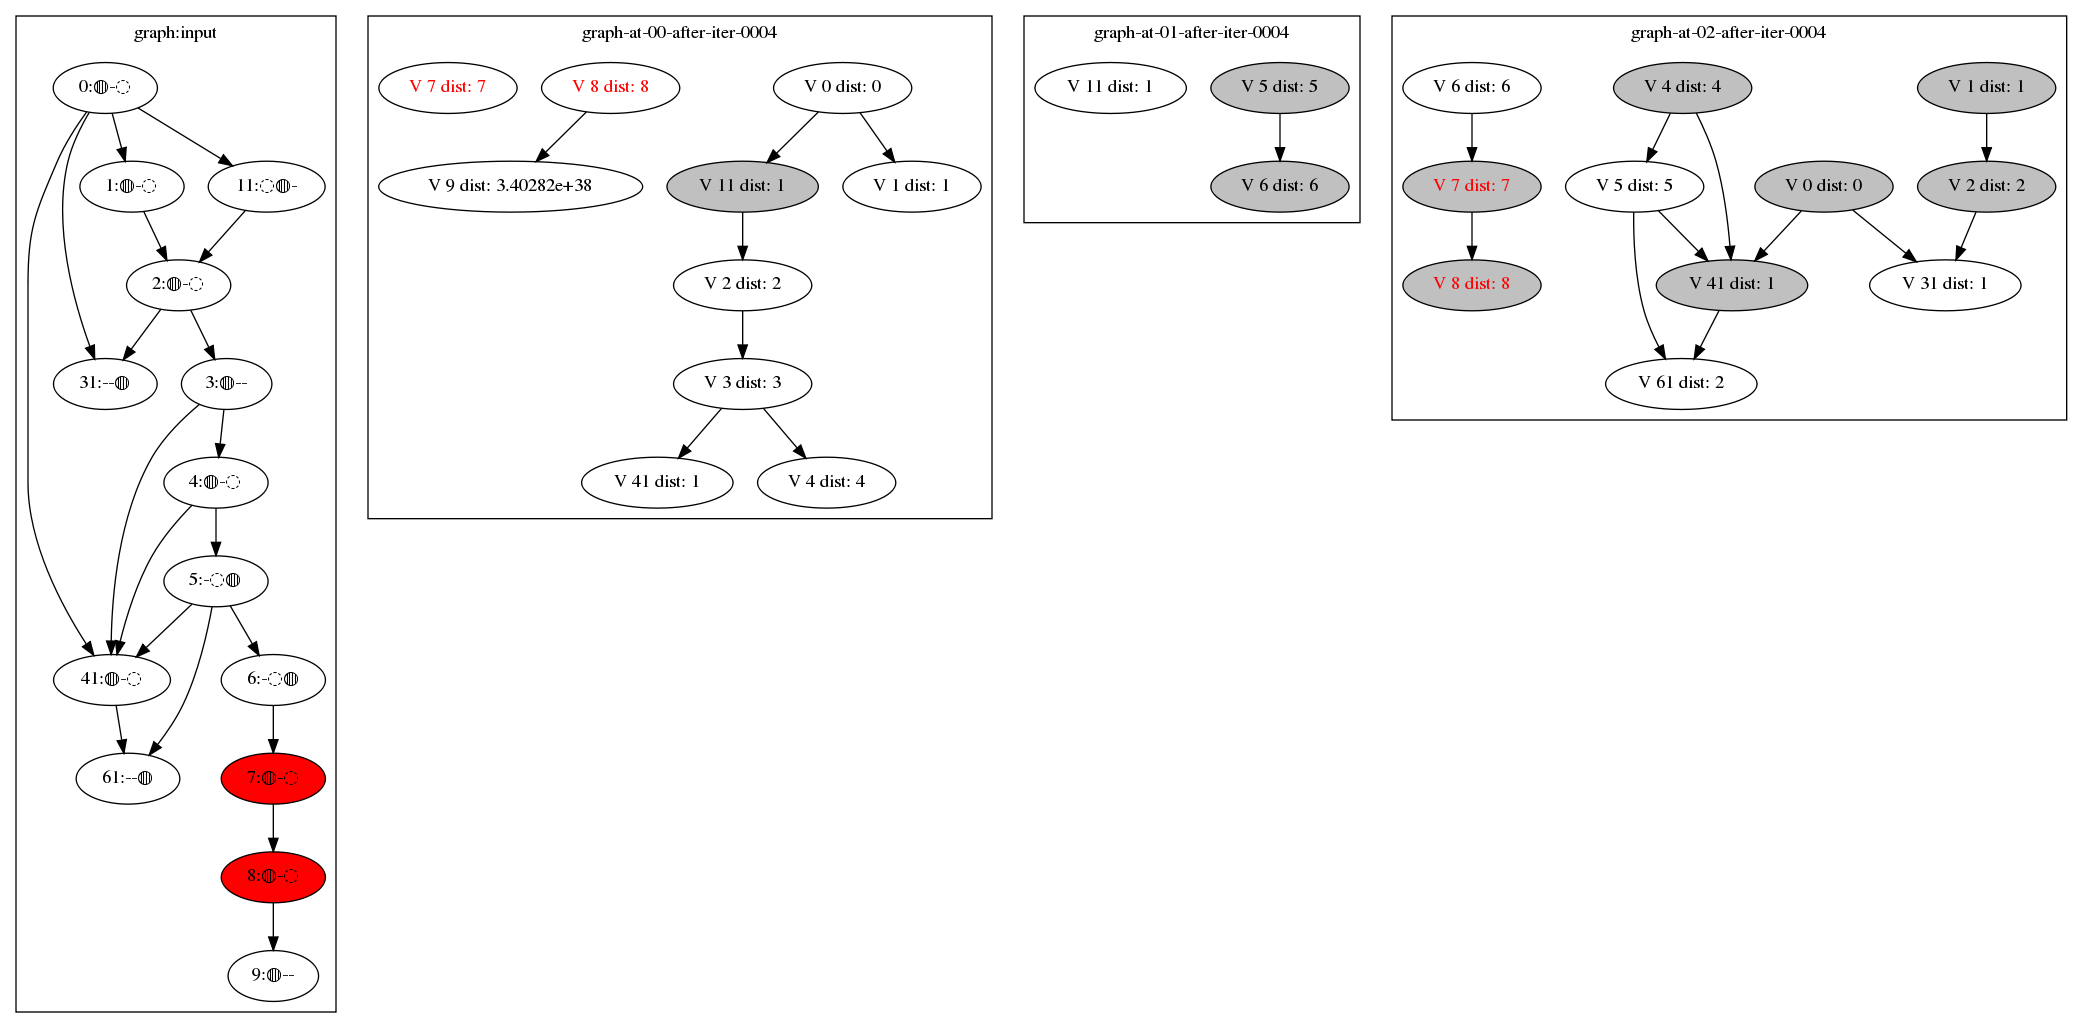
\includegraphics[width=0.8\textwidth]{lazy-iter4.png}    
  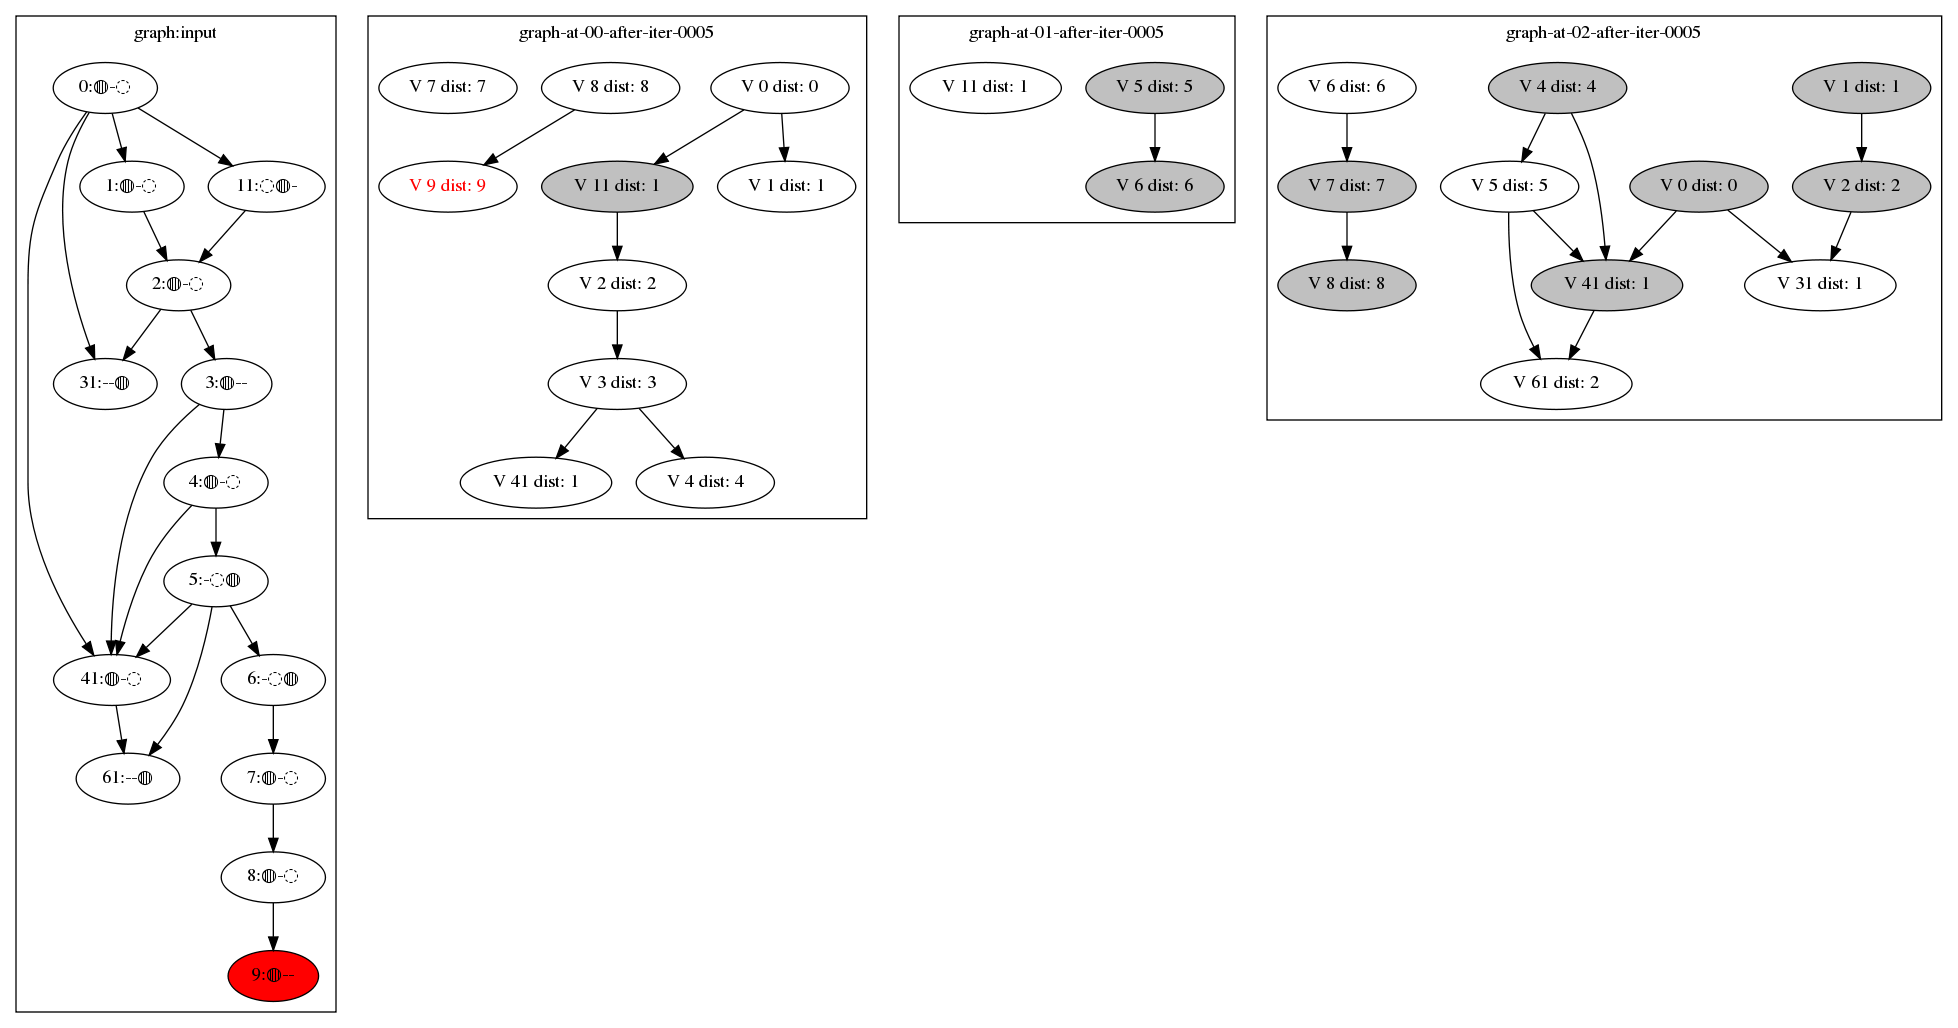
\includegraphics[width=0.8\textwidth]{lazy-iter5.png}
  \captionof{figure}{LazyAsync中SSSP算法的迭代过程}
  \label{fig:sssp-lazy-iter}
\end{center}  


图\ref{fig:sssp-lazy-iter}具体展示了lazy data coherency 中的SSSP算法的迭代运行过程。
还是同样一个由14个顶点和19条边构成的小图,在3台机器上得到划分结果也是一样的,
以0号顶点为source,计算其他顶点到source的最短距离。
一开始和原始的方式一样,系统会把消息值0发送给0号顶点,进而激活0号顶点,把0号顶点作为活跃点参与计算。  
所以第0轮迭代是一样的,机器0上的master 0 激活了自己的本地邻居 master 1 和 mirror 11,
机器2上的mirror 0 激活了自己的本地邻居mirror 41 和 mirror 31。

但是在基于 lazy data coherency 的 LazyAsync中,从第1轮开始,系统的处理方式就和采用 eager data coherency 的同步引擎产生了不同。
在同步引擎中,系统会先收发消息,然后在master上更新顶点数据。
而在LazyAsync中,每次进入新的一轮迭代,系统会先进行本地计算。
在本地计算中,每台机器会先根据自己的本地消息进行互相独立的计算,同时会把本地计算过程中的消息累加起来。

反映在图中,进入第1轮迭代时,
在机器0上存在着上一轮master 0发送给master 1 和 mirror 11的消息,那么本地计算会根据这两个消息把1号顶点和11号顶点
作为活跃点立即进行GAS迭代计算,而mirror 11则会进一步激活它的本地邻居master 2,
然后master 2进一步激活它的本地邻居master 3, 然后 master 3进一步激活它的本地邻居master 41 和 master 4,
而master 1则由于没有本地邻居而不会进一步激活,
这样机器0上不需等待和消息交换经过本地计算之后就已经激活并计算了mirror 11, master 1, 2,3, 4, 41这 6个顶点,
并且此时求得它们顶点上的值分别为1,1,2,2,3,4,4;
在机器1上由于不存在本地消息,也就没有本地计算的过程;
在机器2上存在着上一轮mirror 0发送给master 31 和 mirror 41的消息,那么本地计算会根据这两个消息把41号顶点和31号顶点
作为活跃点立即进行GAS迭代计算,而mirror 41则进一步激活它的本地邻居master 61,而master 31由于没有本地邻居不会进一步激活,
这样机器2上在本地计算阶段激活了mirror 41, master 31, 61,并且此时求得它们顶点上的值分别为1,1,2。

在所有机器上的本地计算都完成之后,系统进入到了数据一致性阶段。
在数据一致性阶段,本地计算中被激活的点都要参与计算进行数据一致。
数据一致性阶段会先对各个活跃点在本地计算期间得到的消息累加和进行交换,
然后活跃点的master副本和mirror副本按收到的消息各自进行一轮独立的GAS计算。
在数据一致性阶段中运行apply部分之后,活跃点的master副本和mirror副本经过计算实现数据一致,
然后活跃点的master和mirror副本会各自运行scatter部分来激活自己的本地邻居,让系统进入下一轮迭代。
反映在图中,我们注意到,经过本地计算除了11,1,31,41之外,系统额外激活并计算了2,3,4,61,并且计算的结果都是准确的。

这里需要注意到,机器0上对master 41进行本地计算得到的是4,而机器2上对mirror41进行本地计算得到的是1,而1才是41号顶点上的正确结果。
显然本地计算之后,正确结果出现在哪个副本上是不确定的,LazyAsync是怎样自动得到了正确的结果呢? 
正是依靠交换本地计算阶段的累加和,使得数据一致性阶段之后,活跃点的master副本和mirror副本上求得的值都是一样的。
这里,机器上0上master 41交换到了机器2上mirror 41记录的本地累加和1从而最终也求得了正确结果1。

第1轮迭代经过本地计算阶段和数据一致性阶段之后,系统进入了第2轮迭代。
在第1轮的数据一致性阶段的scatter计算中,机器0和机器1上的活跃点都没有额外激活本地邻居,因为没有本地消息的产生,
只有机器2上mirror 4激活了本地邻居master 5。
所以在第2轮迭代的本地计算阶段,只有机器2上有本地消息,也就只有机器2进行本地计算。
机器2上的本地计算处理完本地消息后激活并计算了master 5上的值是5,然后本地计算也由于没有需要激活的本地邻居而结束。
在第2轮迭代的数据一致性阶段,mastr 5和mirror5通过消息交换得到了同样的全局视图。

5号顶点进一步激活6号顶点作为第3轮的活跃点,直到最后系统总计经过6轮全局超步迭代之后没有活跃点趋于收敛。
这样,对于同样的输入图,同步引擎需要10轮全局超步迭代,而LazyAsync只用6轮全局超步迭代就能得到同样的正确结果。



以上述这个小图为例,我们在展示LazyAsync的原理的同时,
也看到了这种方法是如何提高图计算效率的。
我们看到 LazyAsync 之所以能够减少全局超步迭代次数是因为
这种方法的本地计算中额外进行了多轮激活迭代。
在同步引擎中,每次迭代之后要进行数据同步和屏障等待才能进入下一轮迭代。
而在LazyAsync中,活跃点的更新是在本地立即可见的,并且这个更新会进一步的激活更多本地活跃点进行计算。
同时由于计算是在本地进行的,不存在网络中的数据交换,读写都是在本地内存中进行,使得本地计算效率更高。
所以LazyAsync相当于在同步引擎中引入了异步引擎的语义\cite{Ju@MACS17},同时又不用像异步引擎那样加全局加锁来维护数据一致\cite{Xie@PPoPP15}。

由于本地计算中更新立即可见并在本地继续传播使得很多活跃点提前收敛,LazyAsync往往能减少图计算的全局超步迭代次数,降低计算时间。
以一个来自snap\cite{SNAP}数据集的大图road-USA-net为例,这是一个包含 2400 万个顶点和5800万条边的大图,
在48机的集群中,采用基于eager data coherency 的同步引擎,对这个图完成 SSSP 计算需要5610轮迭代,耗时1083 s, 
使用基于 lazy data coherency 的 LazyAsync 之后,只需要1604轮迭代,耗时176s,
得到了6倍的加速比。

但是LazyAsync在某些情况下虽然减少了全局超步迭代次数却未必能带来时间上的性能收益。
这一点从总计算时间的构成公式\cite{bsp@1990}中也可以理解:$T=iter \times t_{per\_iter}$。
总时间由$iter$ 和 $t_{per\_iter}$共同影响,如果 $iter$ 减少的同时,$t_{per\_iter}$增大了,
那么总时间就并不一定会减少,甚至会增大。
LazyAsync 能够解释并保证全局超步迭代次数的减少,但它对平均每次超步迭代的时间的影响却是不一定的。
所以LazyAsync需要合适的开启策略才能在减少全局超步迭代次数的同时,也保证不增加甚至减少平均每次迭代时间
这样最终才能得到相对最优的性能提升。

\subsection{冗余计算带来性能损耗}
仍以SSSP为例,本文继续研究了LazyAsync对平均每次全局超步迭代时间的影响。
最终发现,LazyAsync 虽然避免了 eager data coherency 中存在的冗余的同步,等待及通信,
\textbf{但是这种方法却有可能在本地计算过程中引入新的冗余计算}。
本地计算过程中的冗余计算会增加单次超步迭代的计算时间,这样一来LazyAsync虽然减少了图计算过程的全局超步迭代轮次,
但是却最终因为单次全局超步迭代时间的增加而拿不到相对最优的性能提升。


在图\ref{fig:sssp-lazy-iter}中,每一轮全局超步迭代之后本地计算激活的点在数据一致性阶段最终都求得了正确的值。
所以,每次全局超步迭代中的本地计算部分带来的都是性能收益。
然而这只是最理想的情况,实际中考虑到输入图和划分的多样性,
完全存在另一种可能\textbf{使得本地计算中的大部分计算是无效的,
进而使得本地计算带来的是性能损失,最终使得lazy data coherency并不能带来性能收益}。
我们仍以一个小图来说明这种情况。


图\ref{fig:useless}具体展示了LazyAsync的一次全局超步迭代中存在的有效计算与无效(冗余)计算的情况。
在图\ref{fig:useless}中,最左边是一个完整的输入图,右边是这个图划分到2台机器上的情况。
这个划分并不均衡,它是为了演示本地计算中存在的有效计算与无效计算而特意构造的。
但是在实际的图计算中,作为一个子图,这种划分结果是完全可能存在的,
因而这里所演示的情况也是实际会发生的。

在图\ref{fig:useless}中,机器0上的0号顶点收到了本地消息,按照LazyAsync中的本地计算的原则,
机器0上的0号顶点会进一步把本地子图中的连通邻居进一步激活,而机器1上由于没有本地消息则没有进行本地计算。
机器0上本地计算之后,对顶点1,2,21,22,23的计算都是正确有效的,但是对于顶点3,4,5,6,7,8的计算都是错误因而无效的。
并且,其中4,5,6,7,8号顶点的计算无效都是因为对3号顶点的计算无效造成的。
而对3号顶点的无效计算是因为从1号顶点到3号顶点有一条更短的路径,使得3号顶点上的值应为2,
但是由于1-3这条边不在本地,使得本地对计算中对3号顶点的计算是错误的,从而后续的一系列计算都成了无效计算。
最终,在机器0的本地计算中激活了11个顶点,但是只有5个顶点上的计算是有效的,其他6个顶点上的计算是无效的。
这样LazyAsync的本地计算额外多计算了4个点是正确的,但同时也额外多算了6个点是无效的。
这种情况下,LazyAsync虽然还是能够减少全局超步迭代次数,但在本次迭代中执行了不必要的冗余计算,
最终并不能保证得到很好的性能收益。

\begin{center}
  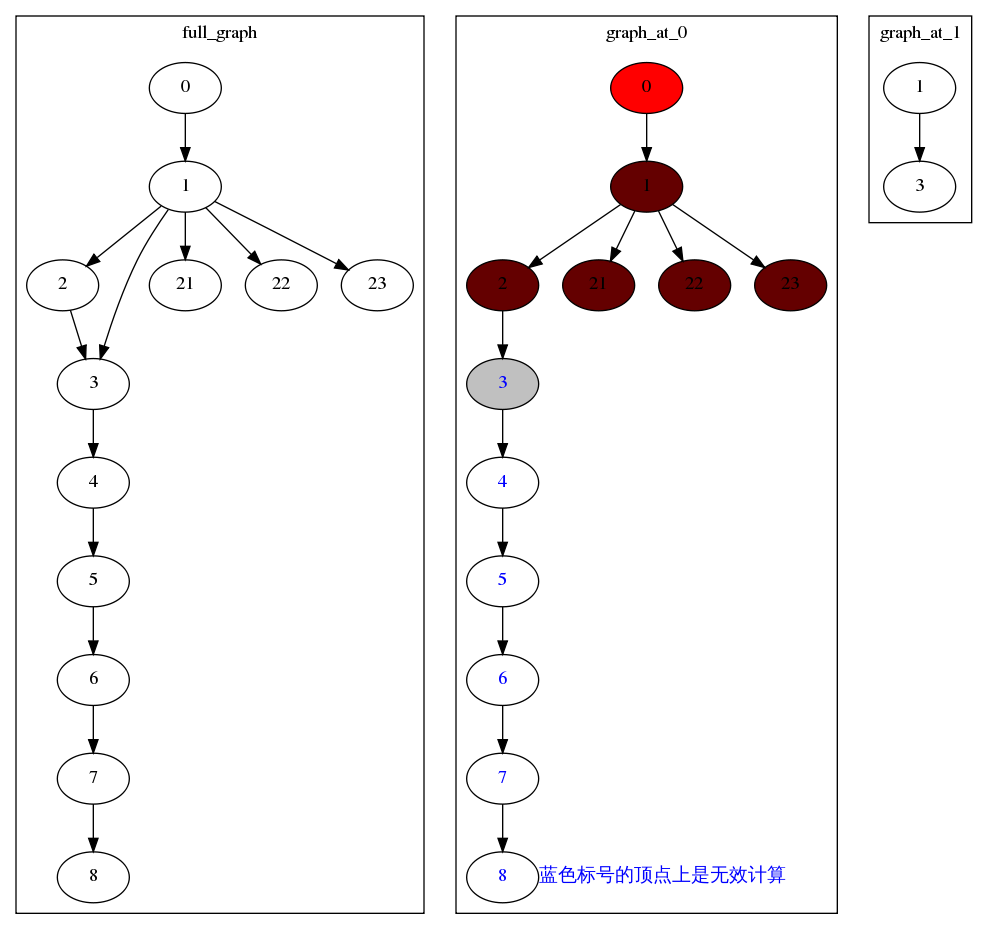
\includegraphics[width=0.8\textwidth]{useless.png}
  \captionof{figure}{有效计算与无效计算示意图}
  \label{fig:useless}
\end{center}  

这里需要额外说明,本地计算中的错误计算最终会被纠正,不会影响最终结果的正确性。
在图\ref{fig:useless}中,本地计算之后,顶点3,4,5,6,7,8上计算的当前值并不等于计算收敛时的正确值。
这在迭代计算中是完全合理的。
并且在本轮数据一致性阶段之后,机器1上的master 1会得到机器0上的mirror 1的正确视图,进而激活master 3。
这样,master 3就在后来的迭代中求得了正确值,并进而正确的激活它的后续邻居,
最终LazyAsync还是能够求得正确结果。

经过以上的分析,我们可以发现,LazyAsync 能够减少图计算的全局超步迭代轮次,提高图计算的计算效率。
但是这种效率的提高受每轮迭代中本地计算的有效程度的影响而不同。
LazyAsync的性能提升来自于它的本地计算能够在本地传播多轮更新值,提前对更多的本地连通点进行计算。
但是,如果本地计算中某些顶点上的值计算错误,那么这些点引起的后续计算都将是错误而无效的
(虽然这些错误最终会在后边的迭代中被纠正)。
这样本地计算带来的就是额外的不必要的性能损失。


\section{通过比较迭代解和最终解量化LazyAsync的性能收益}  

在上一个小节,我们通过一个小图定性地观察了LazyAsync性能收益和性能损耗的来源。
为了探究LazyAsync带来的图计算性能提升程度的规律,我们需要对它的性能收益进行量化。
这里我们采用迭代解和最终解的关系来具体量化LazyAsync的性能收益。

每次全局超步迭代之后,活跃点经过本地计算和数据一致阶段之后会得到一个迭代解。
同时,在算法整体迭代计算结束时,每个顶点都有一个最终解。
我们通过计算每次迭代结束时有效计算的比例,也就是有多少活跃点的迭代解等于最终解,
来对一次全局超步迭代中的LazyAsync的收益进行量化。
显然有效计算的比例越高,LazyAsync的性能收益就越好。
相反,有效计算的比例越低,LazyAsync的性能收益就越差。
在SSSP算法中,对于同步引擎来说,每次全局超步迭代,活跃点经过计算得到的迭代解都等于最终解。
所以,对于同步引擎的SSSP算法来说,有效计算的比例总是为1的。


这其中存在一个问题,最终解是图计算的最终计算结果,是无法事先知道的,只有计算结束时才能得到。
对此,我们让程序先跑一遍把结果存下来,然后再修改程序从结果中读入最终解。
这样每次迭代时,每个顶点都能同时知道它的迭代解和最终解,从而能够比较。
这是为了对LazyAsync的具体效果进行观察而采用的一种技术手段。


\subsection{LazyAsync在不同输入图上的性能收益}

在确定了量化LazyAsync的有效计算比例的手段之后,我们在一些大图上进行了实验来观察比较LazyAsync的性能收益。
在某些本地性比较好的图上,LazyAsync不需要进行手动调优直接开启 lazy data coherency 就能得到相对最优的提升效果。
所以这里主要对比了SSSP算法在本地性不好需要调优的图上调优前后LazyAsync所进行的有效计算的数量和比例。
在本地性不好的图上,立即开启 lazy data coherency 无法得到最好的性能提升,开启的太晚也无法得到最好的性能提升。
本文正是要寻找一种自适应优化方法使得LazyAsync能够在这类图上自动地得到相对最优的性能提升效果。

\begin{figure}[!htbp]
  \centering
  \begin{subfigure}[b]{0.4\textwidth}
    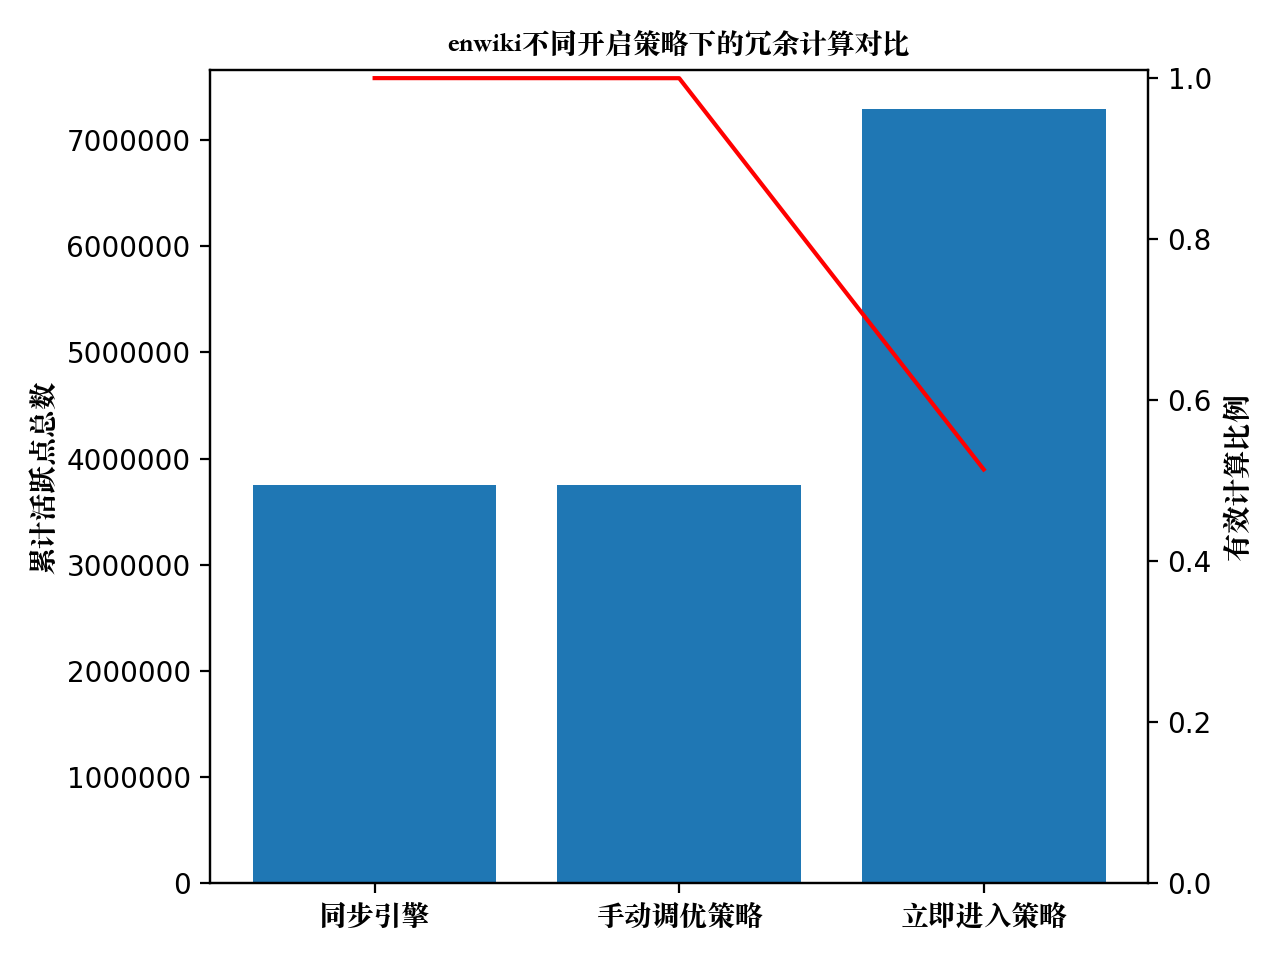
\includegraphics[width=\textwidth]{enwikiuseful}
    \caption{}
    % \label{fig:oaspl_a}
  \end{subfigure}%
  ~% add desired spacing
  \begin{subfigure}[b]{0.4\textwidth}
    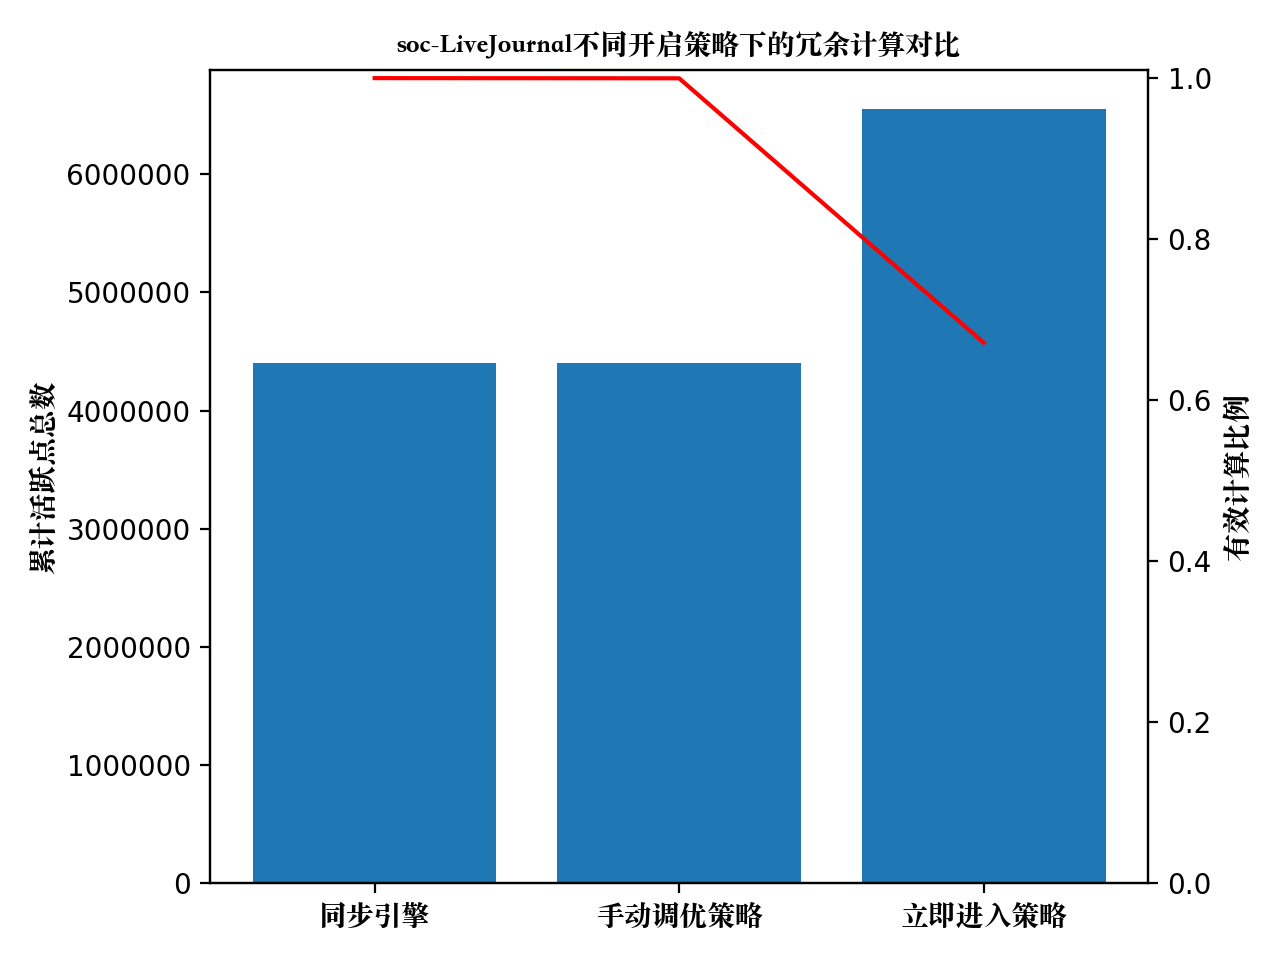
\includegraphics[width=\textwidth]{soc-LiveJournaluseful}
    \caption{}
    % \label{fig:oaspl_b}
  \end{subfigure}
  \\% line break
  \begin{subfigure}[b]{0.4\textwidth}
    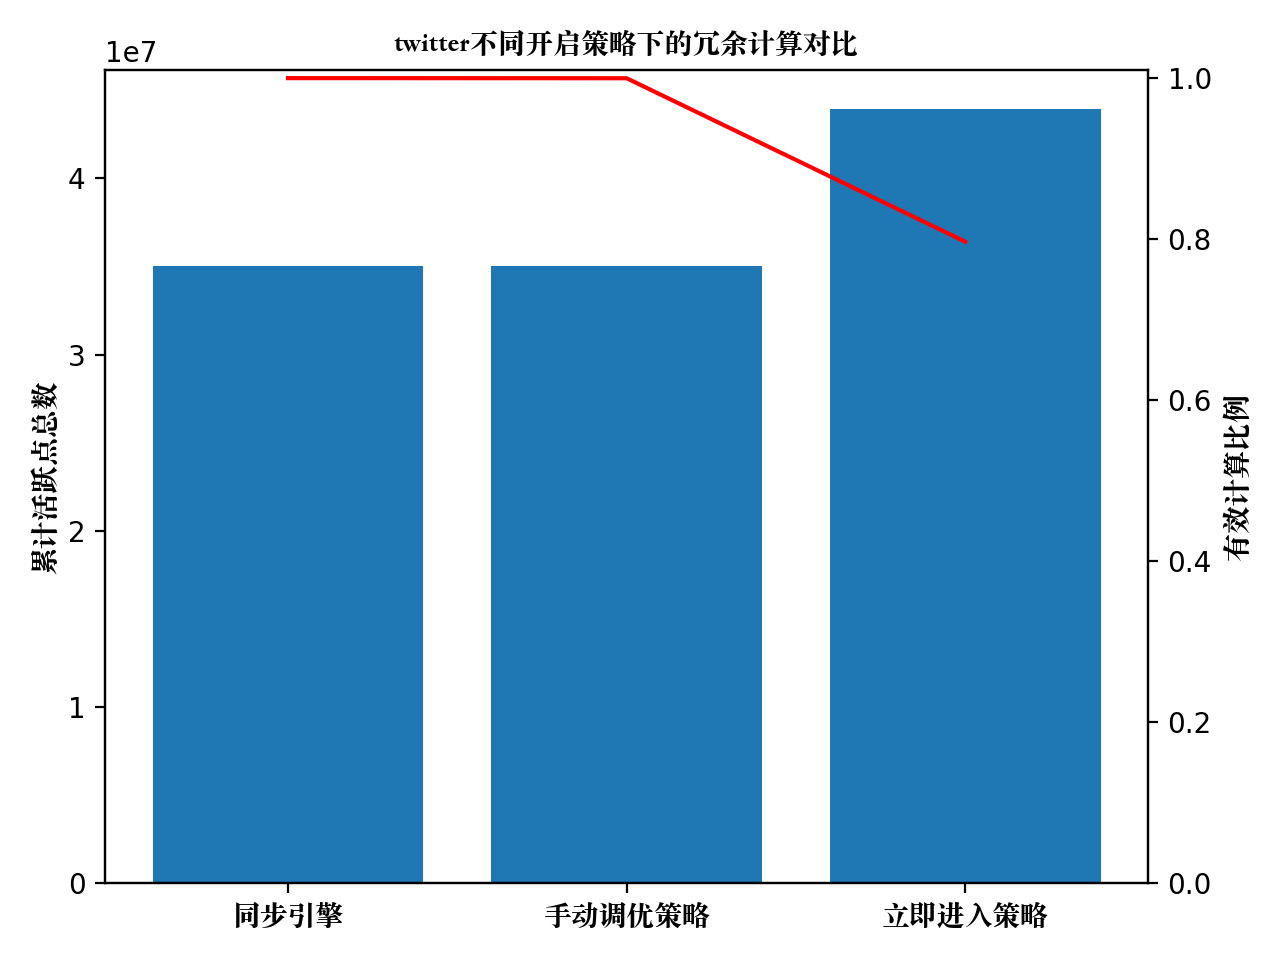
\includegraphics[width=\textwidth]{twitteruseful}
    \caption{}
    % \label{fig:oaspl_c}
  \end{subfigure}%
  ~% add desired spacing
  \begin{subfigure}[b]{0.4\textwidth}
    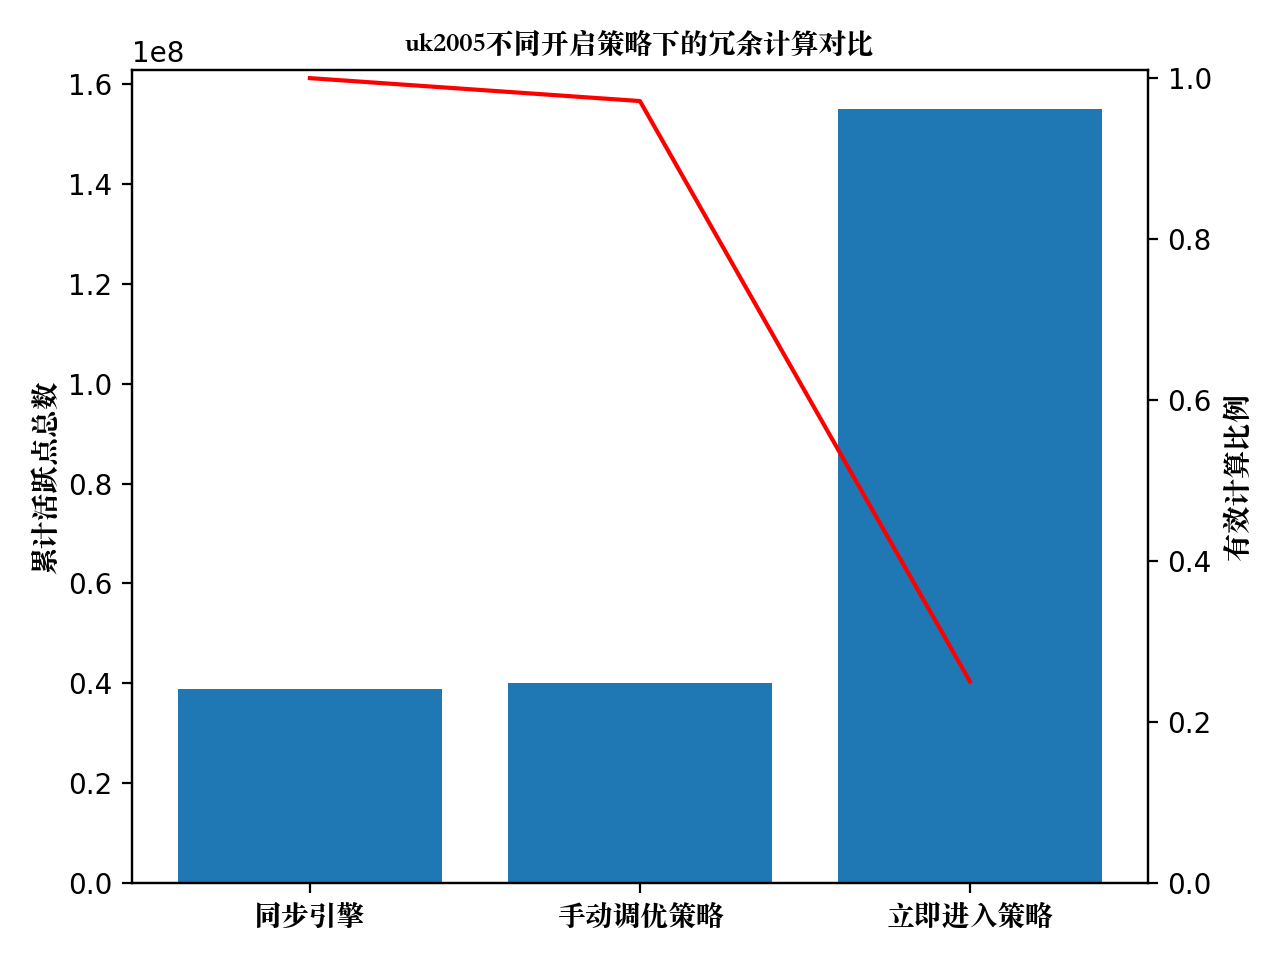
\includegraphics[width=\textwidth]{uk2005useful}
    \caption{}
    % \label{fig:oaspl_d}
  \end{subfigure}
  \bicaption{SSSP 算法在四个图上的冗余计算的比例}{The ratio of redundant calculation of SSSP algorithm on four graphs}
  \label{fig:useful}
\end{figure}


\begin{table}[!htbp]
  \bicaption{SSSP 算法在四个图上的调优效果}{The tuning result of SSSP algorithm on four graphs}
  \label{tab:tuning}
  \centering
  \footnotesize% fontsize
  \setlength{\tabcolsep}{4pt}% column separation
  \renewcommand{\arraystretch}{1.2}%row space 
  \begin{subtable}[t]{0.45\textwidth}
      \centering
      \bicaption{enwiki 上的调优效果}{tuning result on enwiki }
      \label{tab:sample_1}
      \begin{tabular}{lccc}
          \hline
          & iter  & time(s) \\
          \hline
          sync & 53 & 14.24 \\
          \hline
          LazyAsync ,before tuning & 39 & 12.22 \\
          \hline
          LazyAsync ,after tuning & 40 & 9.39 \\
          \hline
      \end{tabular}
  \end{subtable}
  ~% add desired spacing
  \begin{subtable}[t]{0.45\textwidth}
      \centering
      \bicaption{soc-Livejournal 上的调优效果}{tuning result on soc-Livejournal }
      \label{tab:sample_2}
      \begin{tabular}{lccc}
          \hline
          & iter & time(s) \\
          \hline
          sync & 15 & 5.84 \\
          \hline
          LazyAsync ,before tuning & 10 & 5.07 \\
          \hline
          LazyAsync ,after tuning & 13 & 4.21 \\
          \hline
      \end{tabular}
  \end{subtable}
  \\% line break
  \begin{subtable}[t]{0.45\textwidth}
      \centering
      \bicaption{twitter 上的调优效果}{tuning result on twitter }
      \label{tab:sample_3}
      \begin{tabular}{lccc}
          \hline
          & iter  & time(s) \\
          \hline
          sync & 13& 31.63 \\
          \hline
          LazyAsync ,before tuning & 12 & 35.98 \\
          \hline
          LazyAsync ,after tuning & 12 & 24.09 \\
          \hline
      \end{tabular}
  \end{subtable}
  ~% add desired spacing
  \begin{subtable}[t]{0.45\textwidth}
      \centering
      \bicaption{uk-2005 上的调优效果}{tuning result on uk-2005 }
      \label{tab:sample_4}
      \begin{tabular}{lccc}
          \hline
          & iter  & time(s) \\
          \hline
          sync & 201 & 53.07 \\
          \hline
          LazyAsync ,before tuning & 58 & {\color{red}56.14} \\
          \hline
          LazyAsync ,after tuning & 71 & 24.99 \\
          \hline
      \end{tabular}
  \end{subtable}
\end{table}
图\ref{fig:useful}和表\ref{tab:tuning}给出了SSSP算法在4个本地性不好的图上的实验结果。
图中给出了采用eager data coherency 的同步引擎,手动调优策略的LazyAsync,立即进入策略的LazyAsync
这三种情况下,系统在整个计算过程中累计激活的活跃点的数量,和其中有效计算的比例。
图\ref{fig:useful}中的每个子图的左侧坐标轴上对应柱状图给出了三种情况下各自累计激活的活跃点的数量,
右侧坐标轴对应折线图给出了三种情况下各自有效计算的比例。
同步引擎下由于采用了eager data coherency 方法所以其有效计算的比例总为1,其激活的活跃点的数目也代表了实际需要计算的活跃点的数目,
所以同步引擎的数据是基准数据。
表\ref{tab:tuning}则给出了对应的SSSP算法在这4个图上三种情况下各自的全局超步迭代次数和总计算时间。

以 SSSP 算法在 enwiki 这个图上的结果为例,在图\ref{fig:useful}中,
我们可以看到在立即进入的策略下,LazyAsync所进行的有效计算的比例约为50\%,
也就是说这种策略下冗余计算的比例为50\%,有一半数量的活跃点上所进行的计算是无效的。
在具体的实验中甚至可看到,在第2轮全局超步中,系统激活并计算了156万个活跃点,但是只有6万个活跃点上的计算是正确有效的,
剩下的150万个点上的计算都是无效的,其有效计算的比例只有4\%,
像这样的本地计算带来的显然绝大部分都是性能损耗而不是收益。
而在手动调优之后,LazyAsync所进行的有效计算的比例为99.991\%,系统只对327个顶点进行了冗余计算。
在其他三个图上,我们也可以看到类似的结果,即手动调优策略下的LazyAsync所激活的活跃点的数量以及有效计算的比例
都基本接近于同步引擎,
而立即进入策略下的LazyAsync所激活的活跃点的数量则普遍高于同步引擎1.4到4倍,冗余计算的比例则在20\%到80\%之间。
采用立即进入策略的LazyAsync普遍激活了更多的活跃点,并且存在不同程度的冗余计算。

在表\ref{tab:tuning}观察对应的全局超步迭代次数和总计算时间可以看到,相较于同步引擎,
无论是立即进入策略还是手动调优,LazyAsync都减少了全局超步迭代次数和计算时间
(不过在uk-2005这个图上,立即进入策略相比同步引擎虽然减少了迭代次数,但是总的计算时间却增加了一点)。
对比立即进入策略和手动调优策略, 可以看到手动调优之后虽然迭代次数相较于立即进入反而多了,但是最终的计算时间却进一步变少了。
这再次印证之前所提到的公式$T=iter \times t_{per\_iter}$,即计算时间受全局超步迭代次数和单次迭代时间共同影响。
减少迭代次数和降低单次迭代时间都能提高图计算的执行效率,而手动调优正是找到了冗余计算相对较少的情况,降低了单次全局超步迭代的计算时间。


\subsection{LazyAsync的性能提升规律}

通过上一节对图\ref{fig:useful}和表\ref{tab:tuning}的综合分析,我们可以总结出LazyA sync的性能提升规律。
即LazyAsync的性能提升程度主要受本地计算阶段中的冗余计算的比例影响。
不同的开启策略会在本地计算阶段带来不同程度的冗余计算,
手动调优找到的开启策略在本地计算阶段具有更小比例的冗余计算因而能够获得更好的性能提升。

我们之前的工作能很好地解释LazyAsync如何获得性能提升但是却无法回答LazyAsync为何在不同开启策略下性能提升程度不同这一问题。
本文对此进行研究并在本章找到了这一问题的来自于LazyAsync在本地计算阶段引入的冗余计算。
通过分析小图我们提出了冗余计算的概念,
通过比较迭代解和全局解我们对冗余计算的比例进行了量化。
通过实验我们发现性能提升程度更好的开启策略具有更小比例的冗余计算。
这些分析和实验虽然是在SSSP算法上进行的,但是冗余计算的现象和概念在LazyAsync中是普遍存在的。
采用LazyAsync,无论何种图算法在本地计算阶段都有可能由于某个点上不正确的解而引起后续更多的无效计算。

冗余计算解释了LazyAsync在不同开启策略下得到不同程度性能提升的现象,同时也为
LazyAsync的自适应优化问题指明了方向。
既然是冗余计算增加了单次全局超步迭代的计算时间,给LazyAsync带来了性能损耗,
那么解决LazyAsync的自适应优化问题可以从减少冗余计算的角度入手。
本地计算中,如果顶点的解是准确的那么后续额外引起的计算是正确有效的,
如果顶点的解本身就不准确那么后续额外引起的计算往往是冗余无效的。
沿着这个思路,本文在第4章结合全局解和局部解的关系最终提出了基于解的局部性的自适应优化方法。

% \begin{center}
%   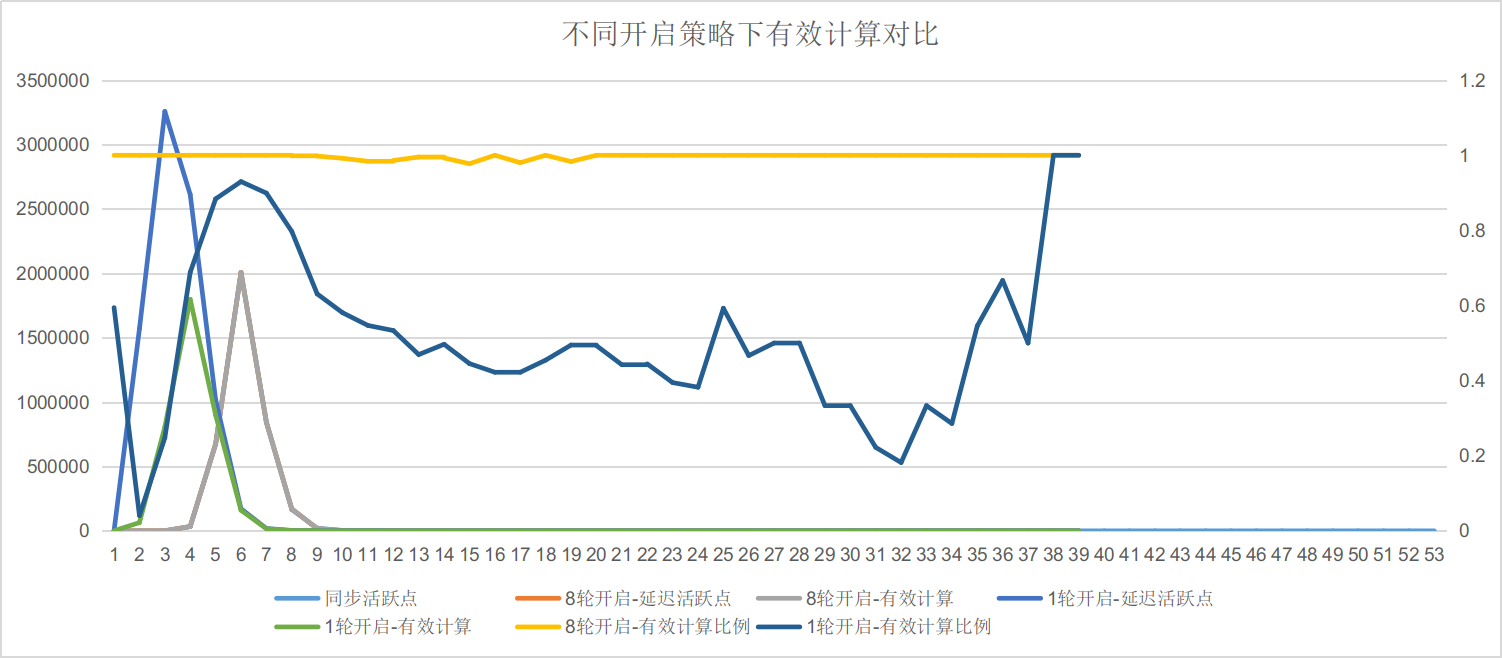
\includegraphics[width=0.8\textwidth]{wiki-lazy.png}
%   \captionof{figure}{enwiki图上不同的开启策略下的有效计算的比例}
%   \label{fig:wiki-lazy}
% \end{center}  

%2020.03.25 02:00

\section{本章小结}
LazyAsync 遗留的主要问题是如何找到合适的开启策略从而得到相对最优的性能提升,这也正是本文所要研究的自适应优化问题。
在本章中,通过在小图上的具体分析和大图上的实验,我们发现延LazyAsync所得到的性能提升程度和冗余计算的比例有关。
LazyAsync避免了原有的 eager data coherency 方法中存在的冗余同步,等待和通信,但是在自己的本地计算中引入了新的冗余计算。
这种冗余计算主要来自于延迟落后的数据在本地所进行的不必要的多轮计算,使得单次全局超步迭代的时间增加,最终影响了LazyAsync的性能提升。
在之前的工作中,我们先是手动调优找到LazyAsync相对最好的性能提升,然后用数据拟合的方法得到一个决策树策略。
但是这些都不能直接指导我们如何得到相对最优的性能提升,
现在我们发现LazyAsync可以通过降低冗余计算比例的方法来得到相对更好的性能提升。

\chapter{基于解的局部性的自适应优化方法}
在上一章中,我们发现了延迟数据一致性方法的性能提升的相对大小和冗余计算的比例有关。
为了得到更好的性能提升,延迟数据一致性方法需要尽可能的避免冗余计算。
在本章中,从如何降低冗余计算比例这一问题出发,本文最终实现了基于解的局部性这一自适应优化方法。
在这一方法指导的开启策略下,延迟数据一致性方法获得了相对最优的性能提升。

在本章中,我们先是从单个顶点的角度出发分析了全局解和局部解的局部性关系有利于减少冗余计算。
然后通过实验对图计算过程中全体活跃点上全局解和局部解的关系进行了分析,发现了解的局部性这一规律。
从这一规律入手,通过在线统计的方法,本文最终实现了基于解的局部性的自适应优化方法。
最后,本章在不同图算法和输入图的组合上对这种方法进行了评测,验证了它的性能提升效果。

\section{全解解和局部解如何影响冗余计算}

在分布式图计算中,由于副本点的存在,每个顶点上的全局解由多个局部解构成。
在把图计算迭代公式改写为差值累加的形式之后,图计算通过交换构成局部解的消息累加值来实现不同副本点上的全局解的一致。

当顶点上的全局解由多个局部解构成时,那么多个局部解都不等于全局解。
那么用这样的局部解进行的本地计算自然是冗余无效的。
当顶点上的全局解由单个局部解构成时,那么这个局部解就等于全局解。
用已经等于全局解的局部解进行本地计算自然是有效的。
同时由于其他副本上没有局部解,副本点就不记录为活跃点,也就不会产生本地计算。
这些副本会在数据一致时收到消息,从而得到和全局解一致的视图。
也就是说就单个顶点而言,全局解由多个局部解构成时不利于开启延迟数据一致性方法,
全局解由单个局部解构成时有利于开启延迟数据一致性方法。


在图\ref{fig:useless_and_local}中,我们再次以 SSSP 为例子直观的展示全局解和局部解如何影响冗余计算。
图\ref{fig:useless_and_local}中,左侧给出了一个全局解由多个局部解构成的例子,右侧给出了一个全局解由单个局部解构成的例子。
在左侧中,一个顶点在5台机器上分布着副本点,并且5台机器上分别存在着6,7,7,8,9这5个局部解。
根据SSSP中对局部解之间$\oplus$的定义:$a\oplus b=std::min(a,b)$,全局解为6。
所以只有一个局部解等于全局解,在机器1,2,3,4上的局部解都不等于全局解。
如果此时对这5个副本点使用延迟数据一致性方法,那么机器1,2,3,4上的副本点所进行的本地计算都是无效而冗余的。
在右侧中,同样是一个顶点在5台机器上分布着副本点,但是只在机器2上存在局部解,此时机器2上的局部解就是全局解。
如果此时对这5个副本使用延迟数据一致性方法,那么机器0,1,3,4上的副本由于没有收到消息不被激活,所以不产生本地计算。
机器2上的副本其局部解就等于全局解,所以机器2上所进行的本地计算是有效的。
在数据一致性时,机器0,1,3,4上的副本会通过消息交换得到和机器2上的副本同样的全局视图。



\begin{figure}[!htbp]
\centering
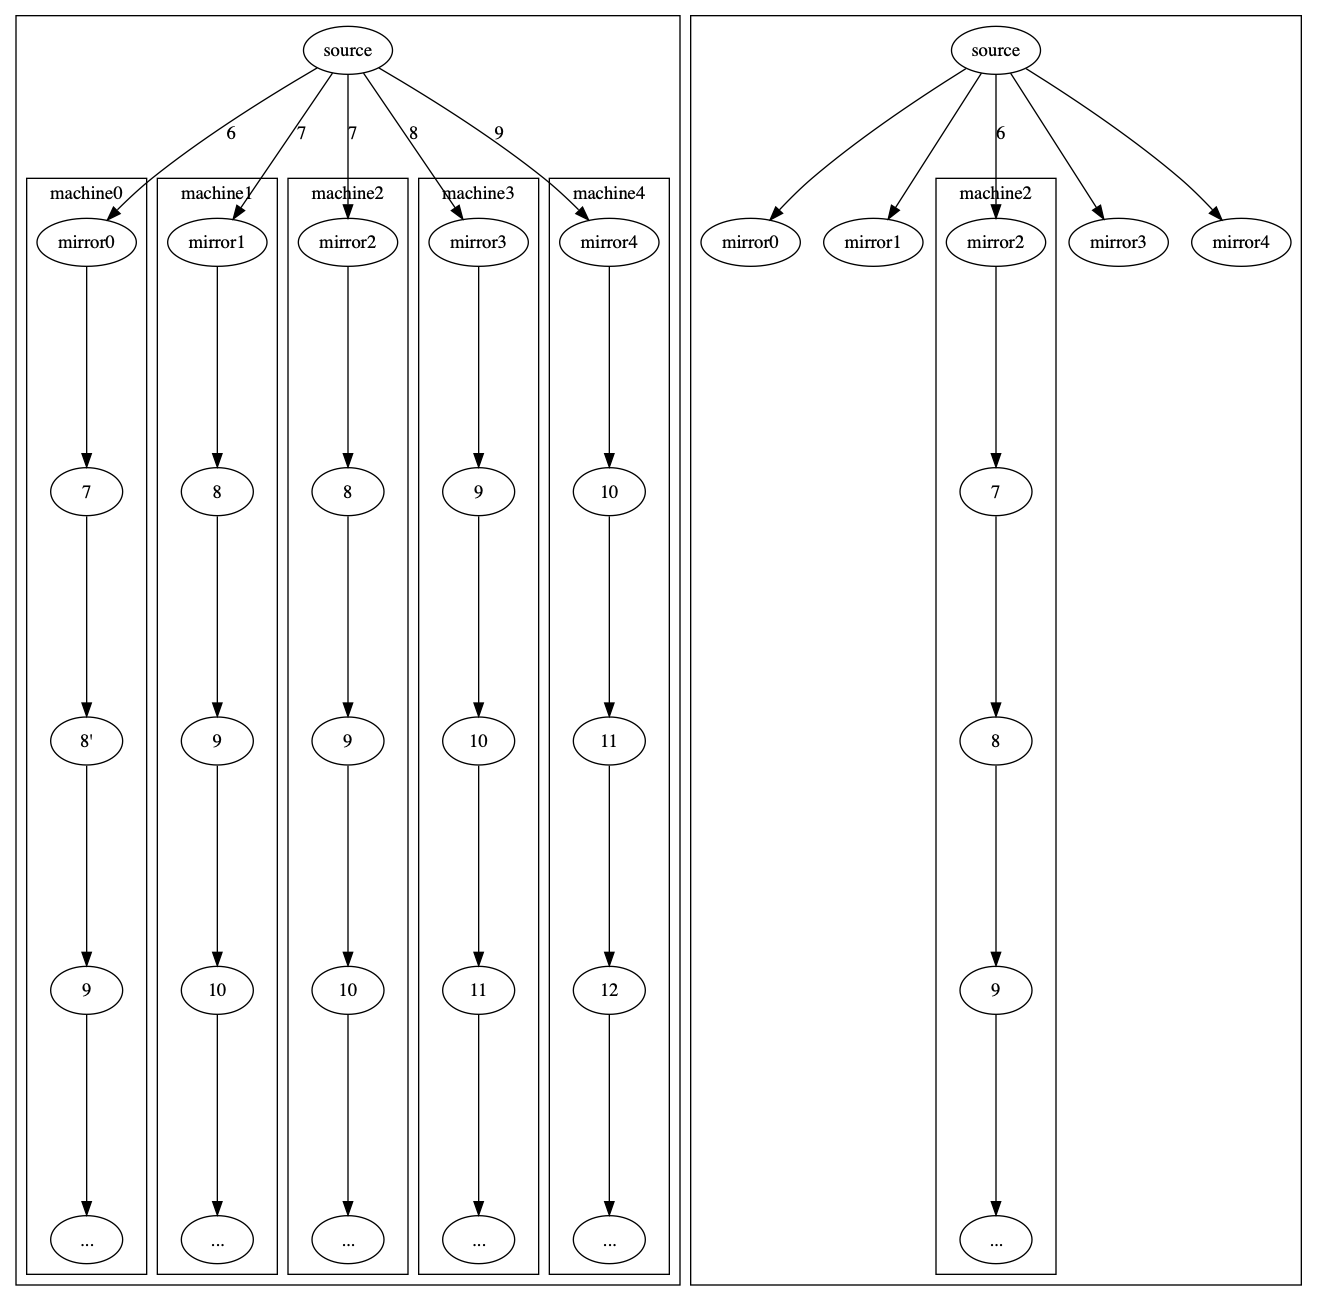
\includegraphics[width=0.8\textwidth]{useless_and_local}
\bicaption{解的局部性如何影响冗余计算}{How the locality of the solution affects redundant calculations}
\label{fig:useless_and_local}
\end{figure}


通过上边的例子我们可以看到,全局解由单个局部解构成时有利于开启延迟数据一致性。
分布式图计算框架把单个顶点划分为多个副本点。
在延迟数据一致性方法中,每次迭代时,顶点的全局解也就由多个副本点上的局部解构成。
从单个顶点的角度而言,
如果顶点的全局解由多个局部解构成,然后此时在各个局部解所在的副本点上进行延迟数据一致性方法,也就是在本地计算中进行额外的多轮迭代,
由于副本点上都是不准确的局部解,因而此时所进行的本地计算都是在不准确的结果上进行的,所以最终本地计算中更多是冗余计算。
相反,如果顶点的全局解只由某个局部解构成,那么在局部解所在的副本点上开启延迟数据一致性方法,
由于局部解就等于全局解,所以此时相当于在全局同步之后进行的迭代,那么此时所进行的本地计算中冗余计算的比例就较低。
也就是说,从单个顶点而言,当全局解只由某个局部解构成时,本地计算中冗余计算比例较低,有利于开启延迟数据一致性方法,
当全局解由多个局部解构成时,本地计算中冗余计算比例较高,不利于开启延迟数据一致性方法。

% 在图计算的每次迭代过程中有很多活跃点,这些活跃点中既有全局解由单个局部解构成的,也有全局解由多个局部解构成的。
在图计算过程中的任何时刻,全局解由单个局部解构成和由多个局部解构成的情况都是同时存在的。
如果大部分活跃点的全局解只由单个局部解构成,那么此时开启延迟数据一致性能够减少冗余计算,最终得到较好的性能提升。
% 但是如果大多数顶点的全局解都只由当局部解构成,那么此时显然是开启延迟数据一致性的良好时机。
对于这种情况,我们称之为解的局部性。
% 这种情况我们称之为解的局部性。

\section{全局解和局部解的关系中的局部性规律}
为了研究图计算过程中解的局部性的变化规律,我们需要保存每次迭代过程中的局部解,然后对其进行观察。

在图计算过程中,局部解由本地的消息累加和构成。
这些消息累加和被包含在消息中然后在集群结点之间进行交换。
消息交换在图计算中起着重要作用,消息中的消息累加和承载了下一轮迭代有哪些活跃点以及这些活跃点收到的消息这些重要信息。
当消息为空时,系统中没有活跃点,图计算也就收敛结束了。

在m2m方式的消息交换中,系统通过三个阶段完成副本点之间的局部解的交换从而实现数据一致。
第一个阶段,所有的副本点向 master 点发送自己的消息累加和。
master 点收到所有副本点上的消息累加和之后按照事先定义的$\oplus$操作符对这些消息累加得到全局消息累加和。
此时进入第二个阶段,master 点向所有副本点发送全局消息累加和。
此时所有的副本点都得到了一份原有的本地消息和全局消息累加和。
由于全局消息累加和中存在着重复的本地消息,所以消息交换还需要第三个阶段,
每个副本点要在全局消息累加和中减去自己的本地消息。
最终经历这三个阶段,每个副本点都得到了相同的消息累加和从而得到相同的全局视图。


可以看到局部解直接体现为副本点的本地消息累加和。
但是图计算过程中并不关心副本点上的消息累加和之间的数量和相对数值,只关心最终的全局消息累加和。
消息交换完成得到全局消息累加和之后,代表着局部解的本地消息累加和就会被清空。
所以,为了记录局部解和全局解从而分析它们的规律,我们需要给 vertex data 添加两个数据结构。
一个是$std::map<int,T> data\_at\_iter$用于记录第$i$次迭代时顶点的全局解。
一个是$std:map<int, std::vector<message\_type>> local\_sum$用于记录第$i$次迭代时
顶点收到的多个消息累加和。

在顶点进行全局的 apply 操作时,系统可以在顶点上记录下全局解。
为了记录消息累加和则需要在两个地方添加代码。
第一处是master点发送自己的本地消息累加和,由于不通过网络交换消息,这里可以直接写入。
第二处是为了记录mirror点向master点通过网络发送的本地消息累加和,需要在收消息的地方添加代码。
通过以上两个地方添加记录消息累加和的代码,保证了对局部解的记录是不重不漏的。 
需要说明的是,局部解的数量有可能少于副本点的数量。
因为那些不被激活的副本点是不会向 master 发送包含本地消息累加和的消息的。


图\ref{fig:local_sssp}给出了一个具体的顶点上记录到的全局解和消息累加和的例子。
图中第一列是顶点id,第二列是最终解,第三列是迭代解,第四列是副本点的数量,接下来是顶点上收到的多个消息累加和,
最后一列是顶点上一轮的迭代解。
以图中3629703号顶点为例,可以看到这个顶点有20个副本,全局解是6,由15个局部解构成,并且其中7个局部解都不等于全局解。
在这样的顶点上使用延迟数据一致性方法显然会造成一定数量的冗余计算。
而以图中411911号顶点为例,可以看到这个顶点也有20个副本,全局解是7,但是只由一个局部解构成。
那么像这样的顶点显然是存在着解的局部性的,使用延迟数据一致性方法不太容易造成冗余计算。


\begin{figure}[!htbp]
  \centering
  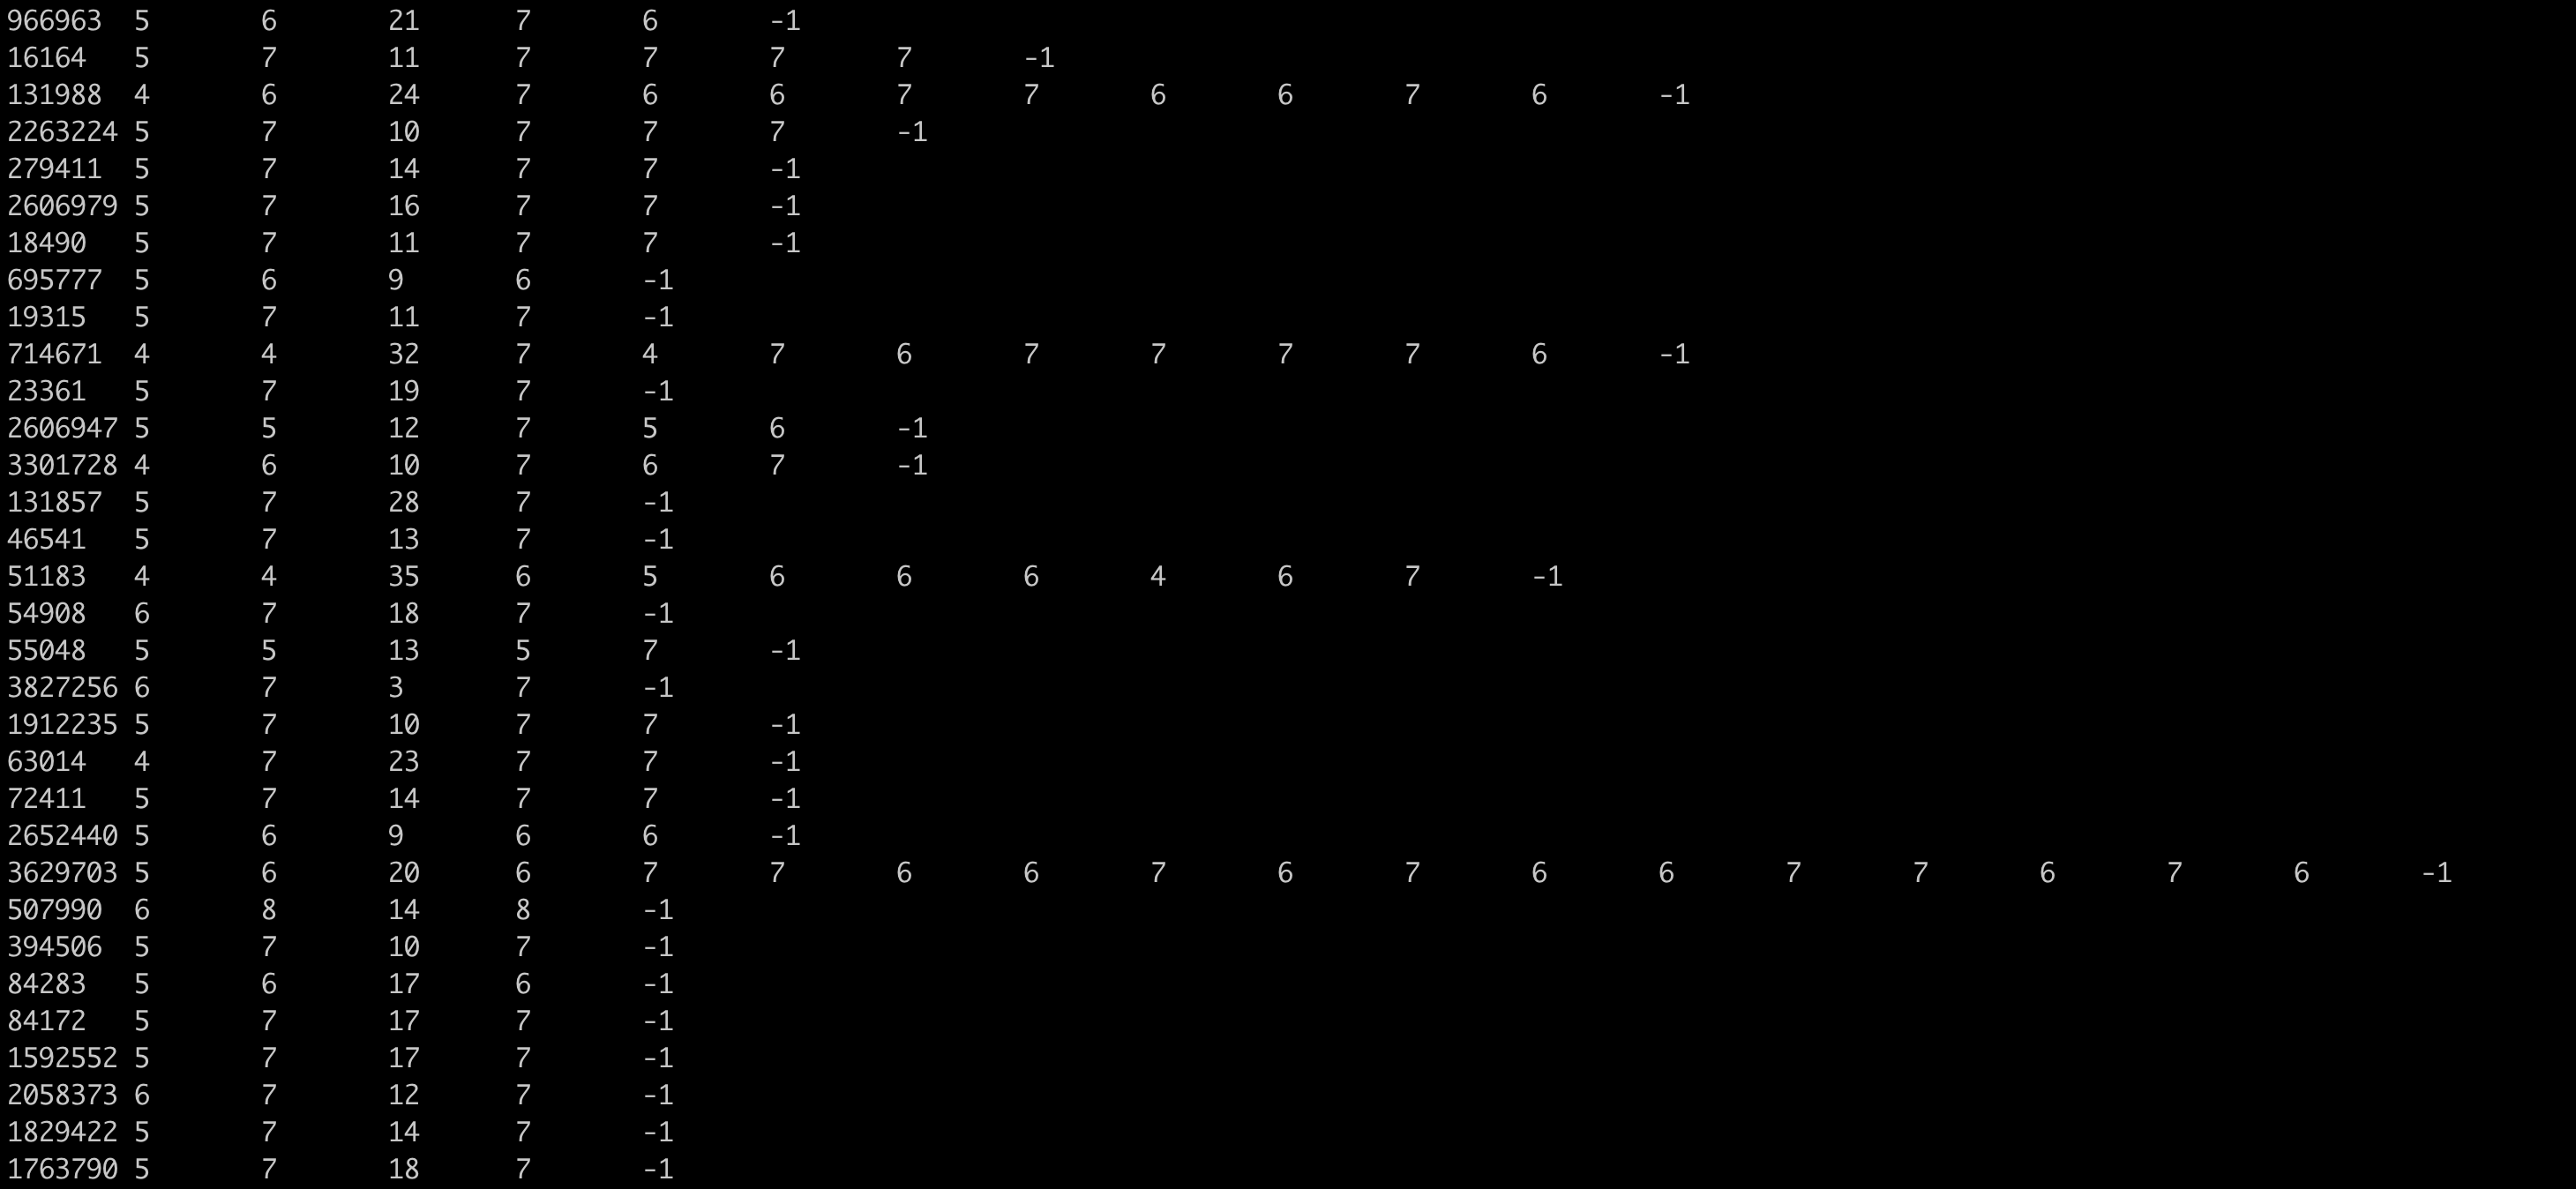
\includegraphics[width=0.8\textwidth]{local_sssp}
  \bicaption{局部解示意图}{Local solution diagram}
  \label{fig:local_sssp}
\end{figure}
%用mapreduce进行统计
通过记录具体的本地消息累加和,我们可以观察在迭代过程中解的局部性的变化规律。
即图计算的迭代过程中,有多少顶点上的全局解是由单个局部解构成的,这样的顶点是否占多数。
图计算完成之后,运行时记录的全局解和局部解这些信息保存在了 graph 中。 
利用 PowerGraph 提供的 map-reduce 接口,我们可以通过 graph 上记录的数据具体统计每一轮迭代中
全局解由多个和单个局部解构成的顶点的数量。

%统计结果


\begin{table}[htb]
  \centering
  \bicaption{实验数据集}{Experimental Data Set }
  \label{tab:experimental_data_set}
    \begin{tabular}{ccccccc}
     \toprule[1.5pt]
     & \textbf{Graph} & \textbf{\#V} & \textbf{\#E} & \textbf{E/V} & \textbf{$\lambda$} } \\
     \midrule[1pt]
     \multirow{2}{*}{web} & UK-2005 & 40M & 936M & 23.73 & 3.51  \\
                                         & web-Google & 0.9M & 5.1M & 5.83 & 2.47 \\
     \cmidrule(lr){1-6}
      \multirow{2}{*}{road} & road-USA-net & 24M & 58M & 2.44 & 2.14 \\
                                          & roadNet-CA & 2M & 5.5M & 2.82 & 2.09 \\
      \cmidrule(lr){1-6}
      \multirow{4}{*}{social} & twitter & 61.58M & 1468M & 23.85 & 5.52 \\
                                          & soc-LiveJournal & 4.84M & 68.9M & 14.23 & 4.96 \\
                                          & enwiki & 4.2M & 101.36M & 24.09M & 7.22 \\
                                          & com-youtube & 1.1M & 6M & 5.27M & 2.70 \\
     \bottomrule[1.5pt]
    \end{tabular}
\end{table}

\begin{figure}[h]
	\centering
  \captionsetup{justification=centering}
  \bisubcaptionbox{ Google 图上的统计结果\label{fig:percent-sssp-google}
}{Statistical results on the Google graph}
{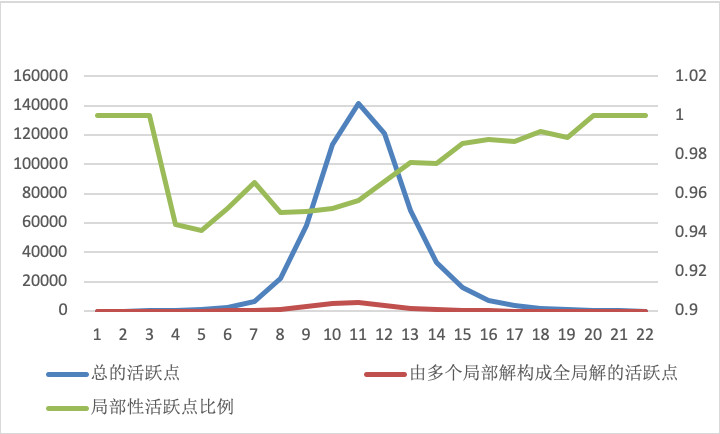
\includegraphics[height=3.8cm,width=0.4\textwidth]{percent-sssp-google.png}}
\hspace{4em}
\bisubcaptionbox{ CA-road 图上的统计结果\label{fig:percent-sssp-ca}
}{Statistical results on the CA-road graph}
{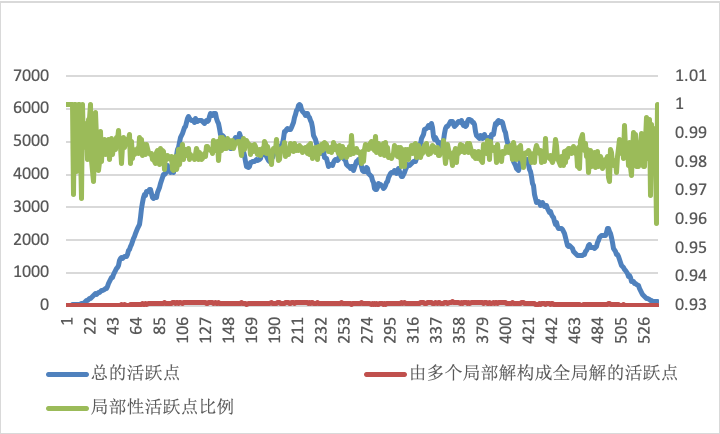
\includegraphics[height=3.8cm,width=0.4\textwidth]{percent-sssp-ca.png}}
\hspace{4em}
\bisubcaptionbox{ youtube 图上的统计结果\label{fig:percent-sssp-youtube}
}{Statistical results on the youtube graph}
{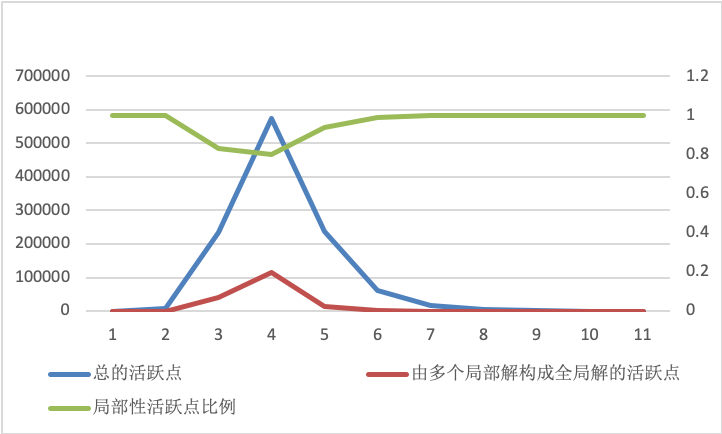
\includegraphics[height=3.8cm,width=0.4\textwidth]{percent-sssp-youtube.png}}
\hspace{4em}
\bisubcaptionbox{ USA-road 图上的统计结果\label{fig:percent-sssp-usa}
}{Statistical results on the USA-road graph}
{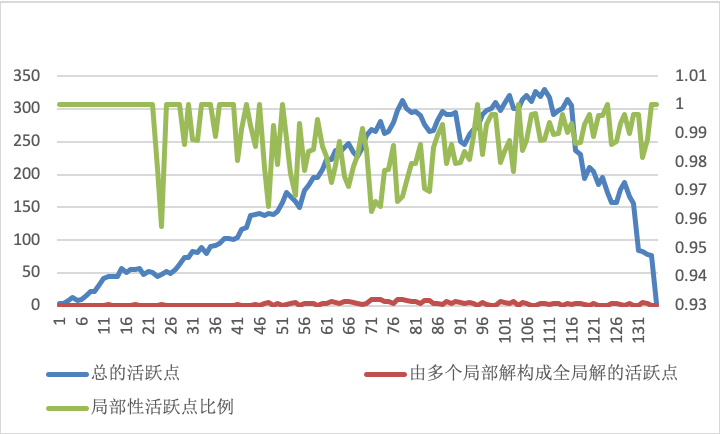
\includegraphics[height=3.8cm,width=0.4\textwidth]{percent-sssp-usa.png}}
\hspace{4em}
\bisubcaptionbox{ soc-Live 图上的统计结果\label{fig:percent-sssp-soc}
}{Statistical results on the soc-Live graph}
{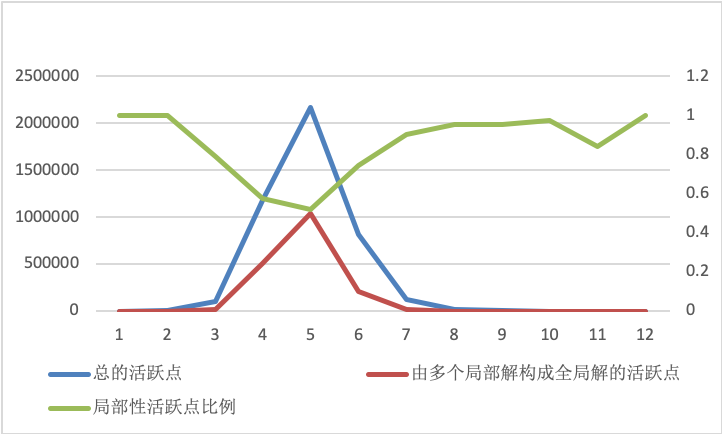
\includegraphics[height=3.8cm,width=0.4\textwidth]{percent-sssp-soc.png}}
\hspace{4em}
\bisubcaptionbox{ enwiki 图上的统计结果\label{fig:percent-sssp-enwiki}
}{Statistical results on the enwiki graph}
{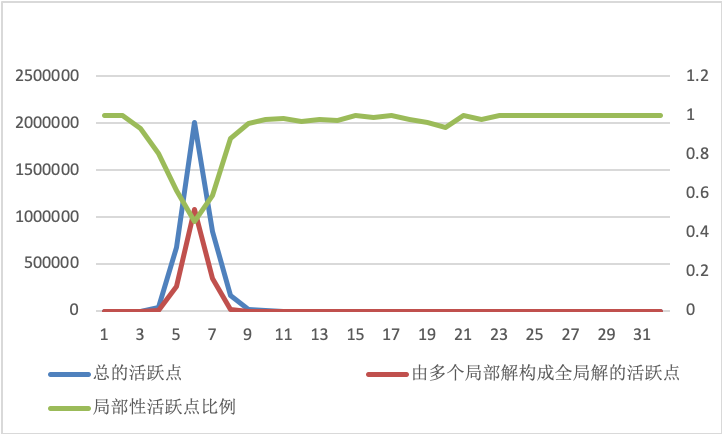
\includegraphics[height=3.8cm,width=0.4\textwidth]{percent-sssp-enwiki.png}}
\hspace{4em}
\bisubcaptionbox{ uk-2005 图上的统计结果\label{fig:percent-sssp-uk}
}{Statistical results on the uk-2005 graph}
{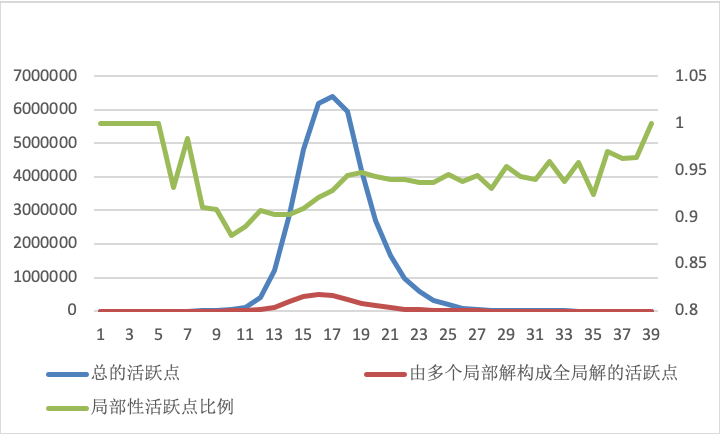
\includegraphics[height=3.8cm,width=0.4\textwidth]{percent-sssp-uk.png}}
\hspace{4em}
\bisubcaptionbox{ twitter 图上的统计结果\label{fig:percent-sssp-ntw}
}{Statistical results on the twitter graph}
{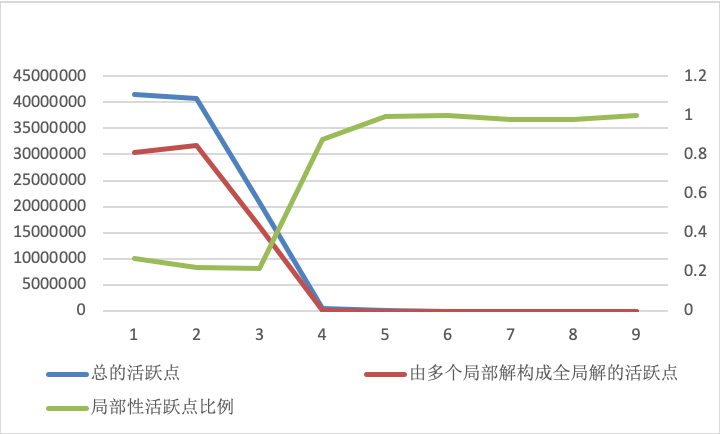
\includegraphics[height=3.8cm,width=0.4\textwidth]{percent-sssp-ntw.png}}
\hspace{4em}

  \bicaption{SSSP 算法在不同图上解的局部性的规律统计结果}{Statistical results for the regularity of local solutions of the SSSP algorithm on different graphs.
}
	\label{fig:percent-sssp}
\end{figure}




\begin{figure}[h]
	\centering
  \captionsetup{justification=centering}
  \bisubcaptionbox{ Google 图上的统计结果\label{fig:percent-cc-google}
}{Statistical results on the Google graph}
{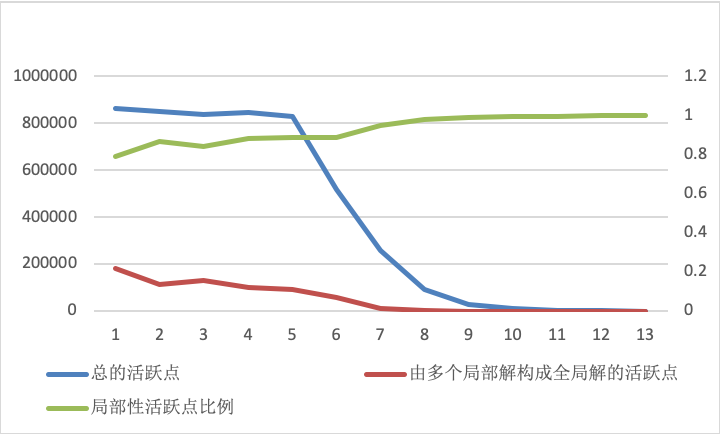
\includegraphics[height=3.8cm,width=0.4\textwidth]{percent-cc-google.png}}
\hspace{4em}
\bisubcaptionbox{ CA-road 图上的统计结果\label{fig:percent-cc-ca}
}{Statistical results on the CA-road graph}
{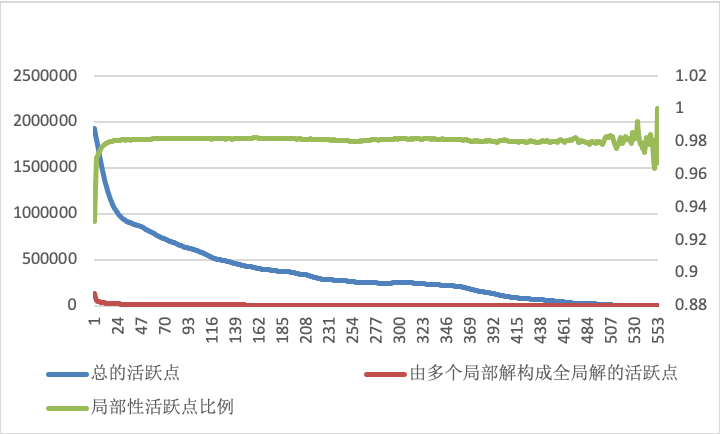
\includegraphics[height=3.8cm,width=0.4\textwidth]{percent-cc-ca.png}}
\hspace{4em}
\bisubcaptionbox{ youtube 图上的统计结果\label{fig:percent-cc-youtube}
}{Statistical results on the youtube graph}
{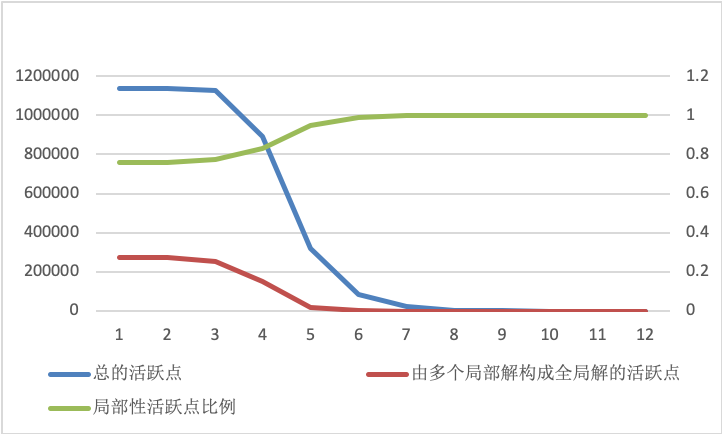
\includegraphics[height=3.8cm,width=0.4\textwidth]{percent-cc-youtube.png}}
\hspace{4em}
\bisubcaptionbox{ USA-road 图上的统计结果\label{fig:percent-cc-usa}
}{Statistical results on the USA-road graph}
{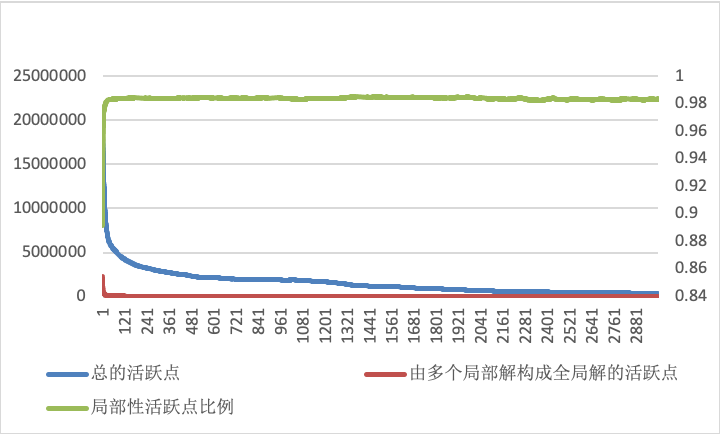
\includegraphics[height=3.8cm,width=0.4\textwidth]{percent-cc-usa.png}}
\hspace{4em}
\bisubcaptionbox{ soc-Live 图上的统计结果\label{fig:percent-cc-soc}
}{Statistical results on the soc-Live graph}
{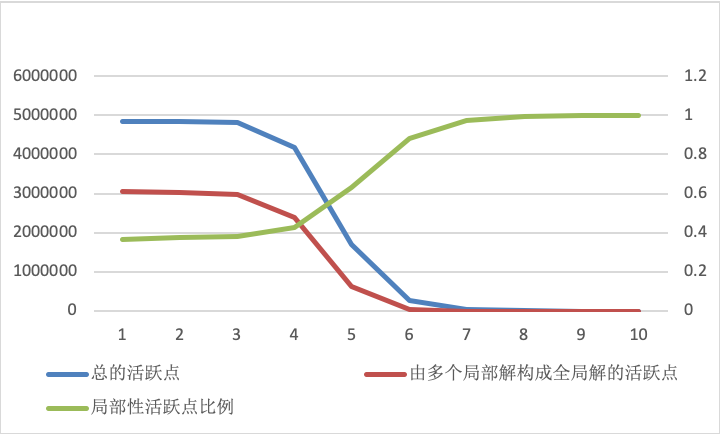
\includegraphics[height=3.8cm,width=0.4\textwidth]{percent-cc-soc.png}}
\hspace{4em}
\bisubcaptionbox{ enwiki 图上的统计结果\label{fig:percent-cc-enwiki}
}{Statistical results on the enwiki graph}
{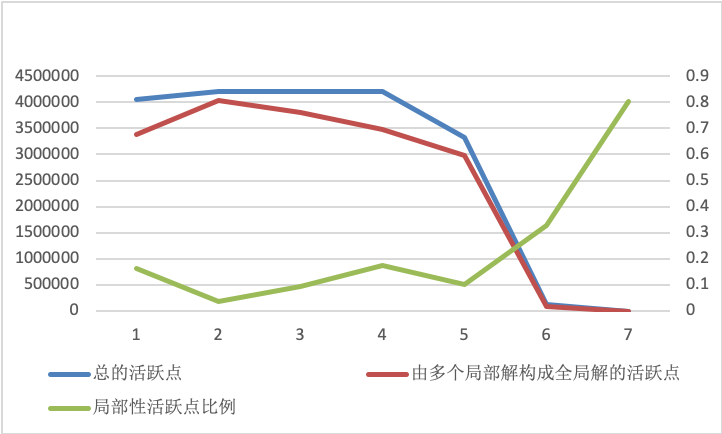
\includegraphics[height=3.8cm,width=0.4\textwidth]{percent-cc-enwiki.png}}
\hspace{4em}
\bisubcaptionbox{ uk-2005 图上的统计结果\label{fig:percent-cc-uk}
}{Statistical results on the uk-2005 graph}
{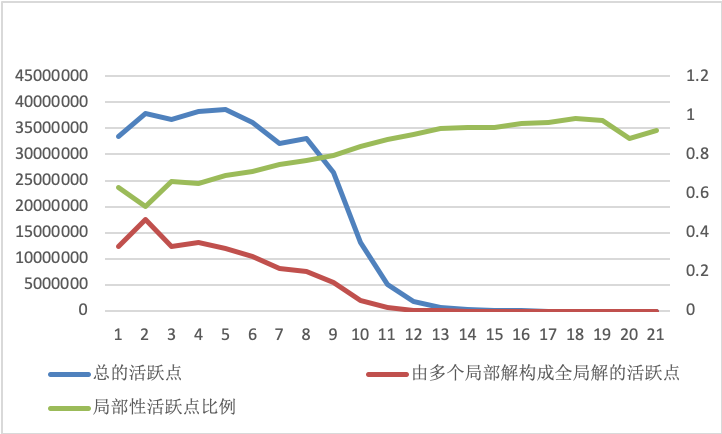
\includegraphics[height=3.8cm,width=0.4\textwidth]{percent-cc-uk.png}}
\hspace{4em}
\bisubcaptionbox{ twitter 图上的统计结果\label{fig:percent-cc-ntw}
}{Statistical results on the twitter graph}
{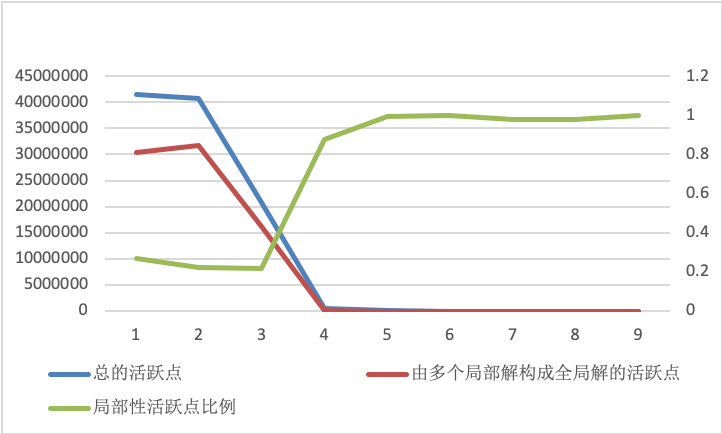
\includegraphics[height=3.8cm,width=0.4\textwidth]{percent-cc-ntw.png}}
\hspace{4em}

  \bicaption{CC 算法在不同图上解的局部性的规律统计结果}{Statistical results for the regularity of local solutions of the CC algorithm on different graphs.
}
	\label{fig:percent-cc}
\end{figure}

\begin{figure}[h]
	\centering
  \captionsetup{justification=centering}
  \bisubcaptionbox{ Google 图上的统计结果\label{fig:percent-pg-google}
}{Statistical results on the Google graph}
{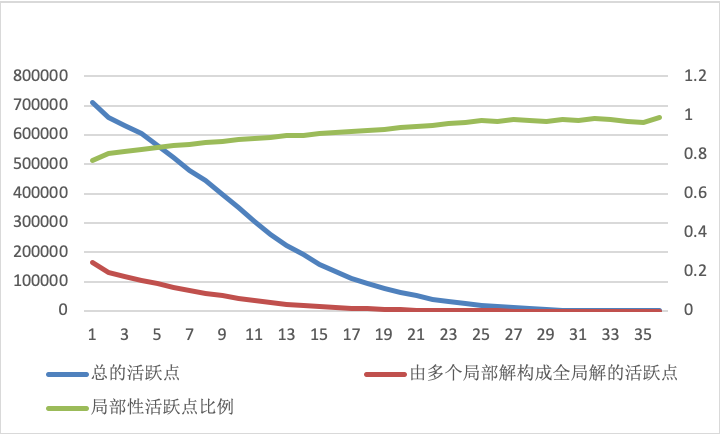
\includegraphics[height=3.8cm,width=0.4\textwidth]{percent-pg-google.png}}
\hspace{4em}
\bisubcaptionbox{ CA-road 图上的统计结果\label{fig:percent-pg-ca}
}{Statistical results on the CA-road graph}
{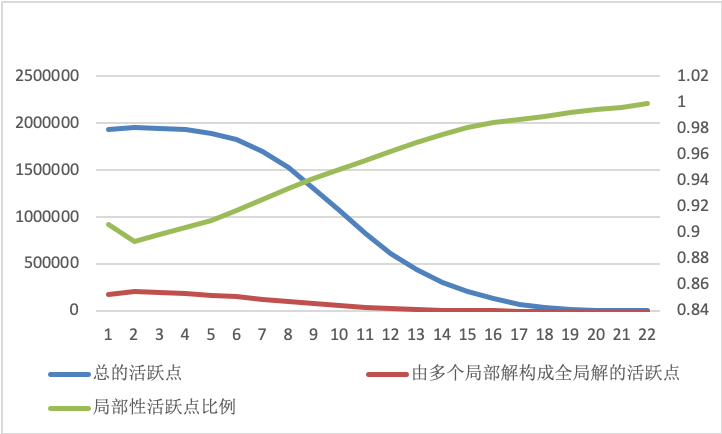
\includegraphics[height=3.8cm,width=0.4\textwidth]{percent-pg-ca.png}}
\hspace{4em}
\bisubcaptionbox{ youtube 图上的统计结果\label{fig:percent-pg-youtube}
}{Statistical results on the youtube graph}
{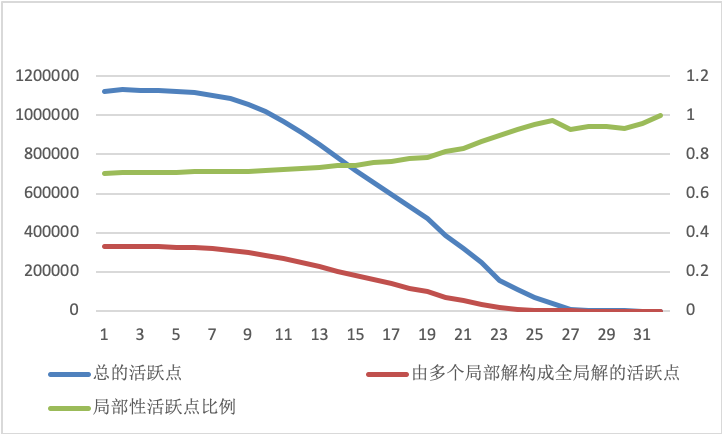
\includegraphics[height=3.8cm,width=0.4\textwidth]{percent-pg-youtube.png}}
\hspace{4em}
\bisubcaptionbox{ USA-road 图上的统计结果\label{fig:percent-pg-usa}
}{Statistical results on the USA-road graph}
{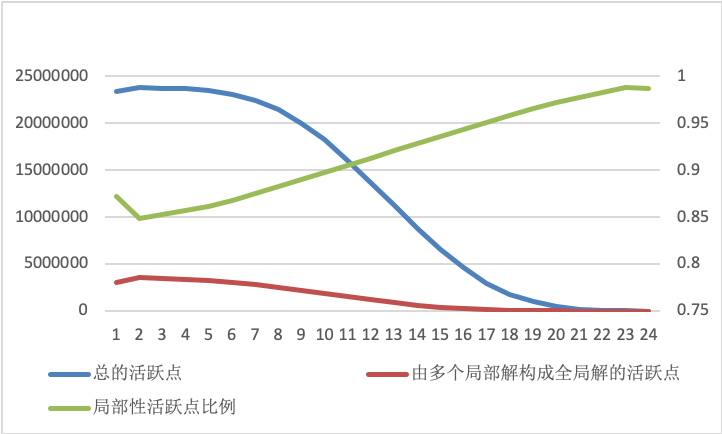
\includegraphics[height=3.8cm,width=0.4\textwidth]{percent-pg-usa.png}}
\hspace{4em}
\bisubcaptionbox{ soc-Live 图上的统计结果\label{fig:percent-pg-soc}
}{Statistical results on the soc-Live graph}
{\includegraphics[height=3.8cm,width=0.4\textwidth]{percent-pg-soc.png}}
\hspace{4em}
\bisubcaptionbox{ enwiki 图上的统计结果\label{fig:percent-pg-enwiki}
}{Statistical results on the enwiki graph}
{\includegraphics[height=3.8cm,width=0.4\textwidth]{percent-pg-enwiki.png}}
\hspace{4em}
\bisubcaptionbox{ uk-2005 图上的统计结果\label{fig:percent-pg-uk}
}{Statistical results on the uk-2005 graph}
{\includegraphics[height=3.8cm,width=0.4\textwidth]{percent-pg-uk.png}}
\hspace{4em}
\bisubcaptionbox{ twitter 图上的统计结果\label{fig:percent-pg-ntw}
}{Statistical results on the twitter graph}
{\includegraphics[height=3.8cm,width=0.4\textwidth]{percent-pg-ntw.png}}
\hspace{4em}

  \bicaption{PageRank 算法在不同图上解的局部性的规律统计结果}{Statistical results for the regularity of local solutions of the PageRank algorithm on different graphs.
}
	\label{fig:percent-pg}
\end{figure}


通过在计算引擎中添加代码和使用map-reduce接口进行统计,本文在SSSP, 
Connected Component(CC),
PageRank 这3种常用的图算法和8个典型的图上进行实验对解的局部性规律进行了统计。
8个图数据集的元数据如表\ref{tab:experimental_data_set}所示,它们包含3个不同类型,下载自
Stanford Large Network Dataset Collection\cite{SNAP}、
the Laboratory for Web Algorithmic \cite{LAW}
和 the DIMACS shortest paths challenge\cite{DIMACS}。

实验结果如图\ref{fig:percent-sssp},\ref{fig:percent-cc},\ref{fig:percent-pg}所示。
图中分别给出了 SSSP,CC,PageRank 算法在 
web-Google, roadNet-CA, com-youtube, USA-road, 
soc-LiveJournal, enwiki, uk-2005, twitter 
这8个大图上关于解的局部性规律的统计结果。
图中每个子图的横坐标轴代表了图计算过程的迭代轮次,
左侧纵坐标轴代表每次迭代的总的活跃点和由多个局部解构成全局解的活跃点的数量,
右侧纵坐标轴代表每次迭代的活跃点中具有局部性规律的活跃点的比例。
活跃点的局部性规律指的是它的全局解只由单个局部解构成。

以图\ref{fig:percent-sssp}(\subref{fig:percent-sssp-google})为例,
这个子图给出了SSSP算法在web-Google图上关于解的局部性规律的统计结果。
图中的蓝色曲线给出了图计算迭代过程中总的活跃点的数量先上升后下降的变化趋势。
图中的红色曲线给出了这些活跃点中由多个局部解构成全局解的活跃点的数量变化趋势。
可以看到在整个图计算过程中,这些由多个局部解构成全局解的活跃点都只占总活跃点数量的一小部分。
图中的绿色曲线则具体给出了图计算迭代过程中由单个局部解构成全局解这样具有解的局部性规律的活跃点的比例。
从图中可以看到,在整个图计算过程中,具有解的局部性规律的活跃点的比例始终在94\%以上。
也就是说在图计算过程中,大部分活跃点的全局解都只由单个局部解构成。

图\ref{fig:percent-sssp}(\subref{fig:percent-sssp-youtube}),
\ref{fig:percent-sssp}(\subref{fig:percent-sssp-ca}),
\ref{fig:percent-sssp}(\subref{fig:percent-sssp-usa})给出了
SSSP算法在 com-youtube,roadNet-CA,USA-road图上的统计数据。
这些图上的统计结果也表明了类似的解的局部性规律,尤其是在
roadNet-CA,USA-road这两张图上,
具有解的局部性规律的活跃点的比例一直保持在96\%以上。

图\ref{fig:percent-sssp}(\subref{fig:percent-sssp-soc})给出了
SSSP算法在soc-LiveJournal图上关于解的局部性规律的统计结果。
和前4个图上的统计结果不同,在soc-LiveJournal图上,
由多个局部解构成全局解的活跃点的数量存在一个明显上升然后下降的趋势,
并且上升的数量使得其在总活跃点中占据较高的比例。
相应地,图中表示具有局部性规律活跃点数量比例的绿色曲线呈现出下降后上升的趋势。
在之前的4个图上,绿色曲线虽然也有波动但是一直保持在90\%以上,
而在soc-LiveJournal这个图上,绿色曲线在下降的最低点达到了50\%,随后逐渐上升接近100\%。
也就是说,在迭代的中间阶段,有相当一部分数量的活跃点的全局解由多个局部解构成,
此时解的局部性规律现象不明显,
到了迭代的后期,红色曲线逐渐上升接近100\%,解的局部性规律现象开始出现。
同时对比三条曲线,我们可以发现,在活跃点开始下降的时候,具有解的局部性规律的活跃点的比例开始上升。

图\ref{fig:percent-sssp}(\subref{fig:percent-sssp-enwiki}),
\ref{fig:percent-sssp}(\subref{fig:percent-sssp-uk}),
\ref{fig:percent-sssp}(\subref{fig:percent-sssp-ntw})给出了
SSSP算法在 enwiki,uk-2005,twitter图上的统计数据。
在这些图上的统计结果上出现了和soc-LiveJournal图上类似的解的局部性规律。
即在一开始活跃点上升的阶段,由多个局部解构成全局解的活跃点的数量也同样上升,并且占据较高比例,
在活跃点下降之后,由多个局部解构成全局解的活跃点的数量也同样下降,并且占据比例下降。
解的局部性规律在活跃点数量下降的后期才开始出现。



图\ref{fig:percent-cc},\ref{fig:percent-pg}分别给出了 
CC,PageRank 算法在 web-Google, roadNet-CA, com- youtube, USA-road, 
soc-LiveJournal, enwiki, uk-2005, twitter 
这8个大图上关于解的局部性规律的统计结果。
由于是不同的图算法,图中活跃点的变化趋势并不相同。
在SSSP算法中,活跃点是从源点开始一层一层激活的,
在CC算法中,邻居点全都会被激活,
在PageRank算法中,则在一开始就激活全部顶点。
同时由于图算法最终都会收敛,所以活跃点最终都会下降为0。
所以在有些图算法上,活跃点会先上升后下降,在有些图算法上活跃点则会一直下降。

不同的图算法在不同输入图上活跃点的变化趋势虽然不同,
但是在图\ref{fig:percent-sssp},\ref{fig:percent-cc},\ref{fig:percent-pg}这些统计结果上,
解的局部性的规律的却是普遍存在的。
只不过在web- Google,roadNet-CA,com-youtube, USA-road 这些图上,
解的局部性规律一开始就存在,即一开始那些由单个局部解构成全局解的活跃点就一直占据较高的比例,
在soc-LiveJournal,enwiki,uk-2005,twitter 这些图上,
解的局部性规律在一开始不明显,由多个局部解构成全局解的活跃点占据较高比例,
直到活跃点数量开始下降的阶段开始,由单个局部解构成全局解的活跃点才占较高的比例,
解的局部性规律才开始出现。


通过以上分析可以得出这样的结论,
在不同的算法和输入图上都存在着典型的解的局部性规律,
即在每轮的活跃点中,大部分顶点的全局解都只由单个局部解构成,由多个局部解构成全局解的顶点只占极少数,甚至没有。

同时,解的局部性规律虽然普遍存在,但却并不是一开始就存在。
在有些图上,由多个局部解构成全局解的点从一开始就只占极少数,并且数量一直在下降。
而在有些图上,由多个局部解构成全局解的点则存在一个先上升后下降的趋势。
也就是说,解的局部性在有的图和算法的组合上是一直都存在的。
而在另外一些图和算法的组合上,则是随着迭代的进行才逐渐出现。
这也是延迟数据一致性方法需要调优才能得到相对最好的性能这一问题的原因。

% 但是在图计算的前期,解的局部性的变化规律则和具体的算法,输入图,以及集群配置有关。

最后,结合图\ref{fig:percent-sssp},\ref{fig:percent-cc},\ref{fig:percent-pg}中的实验结果和之前的决策树策略来分析,
我们发现决策树中选取的特征和实验结果中揭示的规律是一致的。
在决策树策略中,我们使用边和顶点的比例$\frac{e}{v}$来表示图的输入图本地性,
针对那些 $\frac{e}{v} \textless 10$  的图,系统直接开启延迟数据一致性方法,就能获得相对较好的性能提升。
而在我们的实验中发现,在 $\frac{e}{v} \textless 10$ 的web-Google,roadNet-CA,com-youtube,
USA-road 这4个图上,确实一开始就存在着解的局部性的规律。
针对那些 $\frac{e}{v} \textgreater 10$ 的图, 决策树指导系统在活跃点下降率超过7\%时开启延迟数据一致性方法,然后就能获得相对较好的性能提升。
而在我们的实验中发现,在$\frac{e}{v} \textgreater 10$的 soc-LiveJournal,enwiki,uk-2005,twitter 这4个图上,
活跃点下降超过7\%的时间节点,也是由多个局部解构成全局解的活跃点数量开始下降,解的局部性的规律开始出现的时候。

% 同时对于决策树失灵的情况
%结果分析

\section{基于解的局部性的自适应优化方法}


\algnewcommand{\LeftComment}[1]{\Statex \(\triangleright\) #1}

\begin{algorithm}[!htbp]
  \small
  \caption{消息交换中在线统计全局解和局部解关系的算法}\label{alg:exchange_msg}
  \begin{algorithmic}[1] 
      \Require $G(V, E, D)$
      \Require multiLocal:\quad vertex set that contains multiple local soultion 
      \Procedure{ExchangeDeltaMsg}{}
      \LeftComment{Stage1: msg exchange : mirror send deltamsg to  master }

      \For{ \textbf{parallel} v $: has\_message\_global$ }
      \If{ v is mirror }
      \State send deltamsg to master
      \Else{}
      \State append deltamsg to $messages\_global\_sum$
      \State set $has\_message\_global\_sum$

      {\color{red}
      \If{ v in $has\_message\_global\_sum$ }
      \State set multiLocal[v]
      \EndIf
      }

      \EndIf
      \EndFor

      \For{ \textbf{parallel} v $: recv\_buffer$ }
      \State ASSERT\_TRUE(v is master)
      \State append deltamsg to $messages\_global\_sum$
      \State set $has\_message\_global\_sum$
      {\color{red}
      \If{ v in $has\_message\_global\_sum$ }
      \State set multiLocal[v]
      \EndIf
      }
      \EndFor

      \LeftComment{Stage2: msg exchange : master send sum to  mirrors }

      \For{ \textbf{parallel} v $: has\_message\_global\_sum$ }
      \If{ v is master }
      \State send global\_sum to mirrors
      \State set messages \& $has\_message$
      \EndIf
      \EndFor

      \For{ \textbf{parallel} v $: recv\_buffer$ }
      \State set messages \& $has\_message$
      \EndFor
      \EndProcedure
    \end{algorithmic}
\end{algorithm}


\begin{algorithm}[!htbp]
  \small
  \caption{基于解的局部性的自适应优化算法}\label{alg:adaptive}
  \begin{algorithmic}[1] 
      \Require $G(V, E, D)$
      \Require activeCurr:\quad Initial active vertex set activeCurr
      \Require multiLocal:\quad vertex set that contains multiple local soultion 

      % \Ensure output
      \While{$iteration \leq maxIteration$}
      \LeftComment{Stage1: local computation stage}
      \If{$enableLazy \  is \  true$} 
      \For{\textbf{parallel} $activeCurr$}
      \If{$activeCurr \  is \  NULL$ \textbf{or} $doLC() \  is \  false$}
      \State $break$
      \EndIf
      \State $Applys()$
      \State $ScatterGatherMsgs()$
      \State $activeCurr = activeNext$;\quad $activeNext = NULL$
      \EndFor
      \EndIf

      \State $enableLazy = false$

      \State $ExchangeDeltaMsgs()//$详见算法\ref{alg:exchange_msg}
      \State multiLocalCurr = rmi.all\_reduce(multiLocal)
      \State $barrier()$
      \If{$msgEmpty() \  \textbf{and} \  activeEmpty()$}
      \State $break$
      \EndIf
      {
      \color{red}
      \If{ $\frac{e}{v} \textless 10 \quad ||  \quad   multiLocalCurr \textless multiLocalLast $ }
      \State $enableLazy = true$
      \EndIf
      }
      
      \LeftComment{Stage2: data coherency stage}

      \For{\textbf{parallel} $activeCurr$}
      \State $Applys()$
      \State $ScattersGatherMsgs()$
      \State $activeCurr = NULL$
      \EndFor

      \State multiLocalLast = multiLocalCurr
      \State $activeCurr = activeNext$;\quad $activeNext = NULL$; \quad $iteration ++$
      \EndWhile
  \end{algorithmic}
\end{algorithm}

在上一节中,我们通过实验证明了在图计算过程中确实存在着解的局部性规律。
解的局部性这种规律和具体的输入图及算法有关,在迭代的某个时间节点之后才存在。
通过统计全局解由多个局部解构成的顶点的数量,我们可以观察和判断出解的局部性。


延迟数据一致性方法的性能提升受冗余计算的影响。而解的局部性则可以用于减少冗余计算。
基于此,我们最终提出了一种基于解的局部性的自适应优化方法,它指导延迟数据一致性方法
在图计算开始出现的解的局部性的时候来开启延迟数据一致。

在之前的实验中,我们通过保存局部解的方式在图计算完成之后对迭代过程中解的局部性进行观察。
这种事后离线实验的方式只能帮助我们观察图计算过程中的规律,却无法直接作为开启策略。
为了实现基于解的局部性的自适应优化方法,我们需要找到一种在线的统计方式。

在之前的实验中,为了观察局部解的具体数量和数值,我们需要对本地累加和进行记录保存。
但是如果只是为了统计全局解由多个局部解构成的顶点的数量,我们并不需要记录保存本地累加和。
分析消息交换的过程我们发现,只需要在消息交换的过程增加一些判断条件,
我们就能实现在线地统计全局解由多个局部解构成的顶点的数量这一目的。
算法\ref{alg:exchange_msg}给出了我们在消息交换中在线统计全局解和局部解关系这一算法的伪代码,
其中红色部分标出了我们在消息交换过程中添加的判断条件。

如算法\ref{alg:exchange_msg}所示,在消息交换的第一个阶段,标记为mirror的副本点向标记为master的副本点
发送消息。这份消息中包含本地子图的消息累加和,构成了局部解。
同时对于标记为master的副本点而言只需要在本地直接把消息添加到内存的数组中。
对于一个顶点而言,它的全局解由来自master和多个mirror的局部解共同构成。
通过在消息交换第一阶段master顶点接收局部解时判断mater点上是否已经有局部解,我们就能知道
该顶点的全局解是由多个局部解构成还是由单个局部解构成。
当顶点的全局解由单个局部解构成时,这个局部解既可能来自master也可能来自某个mirror。
当顶点的全局解由多个局部解构成时,这些局部解可能只来自部分副本点,因为有些副本点上很有可能未被激活没有局部解。
此外考虑到分布式系统中的消息时延和并发处理的不确定性,我们无法确定来自其他副本的消息和本地master的消息谁更早被写入到内存数组中。

综合考虑以上这些条件,我们在master写本地消息的地方(即算法\ref{alg:exchange_msg} line 8)
和接收远程消息的地方(即算法\ref{alg:exchange_msg} line 17)分别加了判断条件,如果写消息时或收消息时顶点上已经有局部解了,
那么这个顶点上的全局解就由多个局部解构成,相应地要将 multiLocal 这个 bitset 进行标记置位。
在消息发送的第一阶段,本地写消息和接收远程消息都只发生在标记为master的副本点上,对全局解和局部解关系的判断也只发生在标记为master的副本点上。
在消息交换整个阶段完成之后,各个活跃点的副本点都得到了相同的消息累加和,同时那些由多个局部解构成全局解的顶点也已经被标记置位。
此时,通过mpi提供的all\_reduce操作对集群中各个结点的进程实例中的multiLocal进行规约求和,
我们就基于在线统计的方法得到了上一轮迭代中由多个局部解构成全局解的顶点的数量。
相较于4.3节中采用的离线统计方法,这种方法不需要在顶点上额外保存变量,也不需要导出文件,不影响计算过程,
只需要在消息交换中添加if判断条件并进行一个mpi提供的all\_reduce规约操作,开销很小。



实现了在线即时统计全局解由多个局部解构成的顶点的数量这一目的之后,
我们就真正的得到了一个基于解的局部性的自适应优化方法。
这个基于解的局部性的自适应优化方法由算法\ref{alg:exchange_msg}和算法\ref{alg:adaptive}共同构成。
在算法\ref{alg:exchange_msg}的基础上,算法\ref{alg:adaptive}给出了系统如何根据
图的本地性($\frac{e}{v}$)和全局解由多个局部解构成的顶点的数量这两个指标自适应地判断是否启用LazyAsync这一过程的伪代码。
不同的输入图其边点数量比$\frac{e}{v}$各不相同,所以图的本地性这个指标反映了对输入图的自适应。
集群环境和划分算法以及算法用例则会对副本点和副本点上的局部解产生影响,
所以全局解由多个局部解构成的顶点的数量变化趋势这个指标反映了对运行环境变化的自适应。

在算法\ref{alg:adaptive}中我们可以看到,基于解的局部性的自适应优化方法的关键代码其实就是对两个指标的进行的if判断。
但是这个判断正是对4.2节实验中发现的解的局部性变化规律的应用。
在4.2节我们通过实验发现,那些本地性指标$\frac{e}{v} \textless 10$ 的图在各种算法上在迭代一开始就一直表现出明显的解的局部性现象,
所以我们在自适应优化方法中判断立即启用LazyAsync。
对那些本地性指标$\frac{e}{v} \textgreater 10$ 的图,通过实验我们发现,在全局解由多个局部解构成的顶点的数量开始下降时,
由单个局部解构成全局解这样具有解的局部性规律的活跃点的比例开始上升并趋近100\%。
所以在自适应优化方法中我们在观察到$  multiLocalCurr \textless multiLocalLast$ 这一条件时才启用LazyAsync。


\section{性能评测}

在本节中,我们在48台虚拟机构成的集群环境中,对比了PowerGraph原始的同步引擎,
LazyGraph的手动调优方法和LazyGraph的自适应优化方法
这三种方式下的性能。

\subsection{实验环境}
\begin{table}[htb]
  \centering
  \bicaption{实验平台}{Experimental Methodology}
  \label{tab:experimental_methodology}
    \begin{tabular}{cccccc}
     \toprule[1.5pt]
     \multicolumn{5}{c}{\textbf{Each Node}} &   \multirow{2}{*}{\textbf{Cluster}} \\
     \cmidrule(lr){1-5}
     Compiler & CPU & Memory & System & Network \\
     \midrule[1pt]
     GCC 4.4.7 & 8 Intel Xeon cores & 32GB & CentOS 6.5  & 1 GigE Ethernet & 48-node cluster\\
     \bottomrule[1.5pt]
    \end{tabular}
\end{table}



\begin{table}[htb]
  \centering
  \bicaption{实验数据集及划分算法}{Experimental Data Set and Partition Algorithm}
  \label{tab:experimental_data_set_and_partition_algorithm}
    \begin{tabular}{ccccccc}
     \toprule[1.5pt]
     & \textbf{Graph} & \textbf{\#V} & \textbf{\#E} & \textbf{E/V} & \textbf{$\lambda$} & {\textbf{Partition Algorithm}} \\
     \midrule[1pt]
     \multirow{2}{*}{web} & UK-2005 & 40M & 936M & 23.73 & 3.51 & \multirow{8}{*}{Coordinated Vertex-Cut } \\
                                         & web-Google & 0.9M & 5.1M & 5.83 & 2.47 \\
     \cmidrule(lr){1-6}
      \multirow{2}{*}{road} & road-USA-net & 24M & 58M & 2.44 & 2.14 \\
                                          & roadNet-CA & 2M & 5.5M & 2.82 & 2.09 \\
      \cmidrule(lr){1-6}
      \multirow{4}{*}{social} & twitter & 61.58M & 1468M & 23.85 & 5.52 \\
                                          & soc-LiveJournal & 4.84M & 68.9M & 14.23 & 4.96 \\
                                          & enwiki & 4.2M & 101.36M & 24.09M & 7.22 \\
                                          & com-youtube & 1.1M & 6M & 5.27M & 2.70 \\
     \bottomrule[1.5pt]
    \end{tabular}
\end{table}

为了评测本文所提出的自适应优化方法的效果,我们在由48台虚拟机构成的集群环境中测试了
PowerGraph的原始同步引擎,LazyGraph的手动调优方法,和基于解的局部性的自适应优化方法
这三种方式下的性能结果。
如表\ref{tab:experimental_methodology}所示,每个节点上的操作系统是Centos 6.5,
配置的编译器版本为4.4.7,配置的CPU有8个核,内存有32GB,
集群的节点之间以1GigE的以太网连接。
实验过程中使用的数据集总共包含3个类型,8个不同大小的真实图。
这些数据集同4.2节中使用的一样,具体元数据如表\ref{tab:experimental_data_set_and_partition_algorithm}所示。
同时,我们均使用 coordinated vertex-cut 划分算法来做图的划分。
实验过程中使用了
SSSP, 
Connected Component(CC),
K-core Decomposition(kcore), 
Page Rank这四种典型的图算法来作为测试用例。


\subsection{实验结果}

\begin{figure}[h]
	\centering
  \captionsetup{justification=centering}
	\bisubcaptionbox{ SSSP 的加速比\label{fig:speedup_sssp}}{Speedup in SSSP}
	%[3cm] %标题的长度,超过则会换行,如下一个小图。
	{\includegraphics[height=4.5cm,width=0.4\textwidth]{speedup_sssp.png}}
  \hspace{4em}% 这里记得不要空行,否则会变为垂直的两个图
	\bisubcaptionbox{CC 的加速比\label{fig:speedup_cc}}{Speedup in CC}
	%[3cm] %标题的长度,超过则会换行,如下一个小图。
	{\includegraphics[height=4.5cm,width=0.4\textwidth]{speedup_cc.png}}
	\hspace{4em}% 这里记得不要空行,否则会变为垂直的两个图
	\bisubcaptionbox{K-Core 的加速比\label{fig:speedup_kcore}}{Speedup in K-Core}
	%[3cm] %标题的长度,超过则会换行,如下一个小图。
	{\includegraphics[height=4.5cm,width=0.4\textwidth]{speedup_kcore.png}}
	\hspace{4em}% 这里记得不要空行,否则会变为垂直的两个图
	\bisubcaptionbox{PageRank 的加速比\label{fig:speedup_pagerank}}{Speedup in PageRank}
	{\includegraphics[height=4.5cm,width=0.4\textwidth]{speedup_pagerank.png}}
	\bicaption{ SSSP,CC,K-Core和PageRank 在48机真实图上的性能对比}{Speedup Comparisons for SSSP, CC ,K-Core and  PageRank on Real-World Graphs on 48 Machines}
	\label{fig:speedup_four_algorithm}
\end{figure}


\begin{figure}[h]
  \centering
  \captionsetup{justification=centering}
  \includegraphics[width=0.8\textwidth]{sssp-uk-dt-vs-opt}
  \bicaption{不同集群配置下,SSSP 算法在 uk-2005输入图上的运行时间}{Runtime of the SSP algorithm on the uk-2005 input graph with different cluster configurations}
  \label{fig:dt-vs-opt}
\end{figure}

图 \ref{fig:speedup_four_algorithm} 展示了四种图算法在8个不同的输入图上分别采用
PowerGraph 原始同步引擎,
LazyGraph 手动调优方法,
LazyGraph 基于解的局部性的自适应优化方法
这三种方式进行计算所得到的性能测试结果。
可以看到,
在不同的算法和输入图的组合上,LazyGraph的表现性能都好于PowerGraph。
而在LazyGraph 上, 基于解的局部性的自适应优化方法
得到的性能提升效果
和手动调优方式下得到的相当,甚至有时超过了后者。

在手动调优的方法中,我们通过不断的尝试分别在不同的迭代轮次开启延迟数据一致性方法然后取其中最好的值作为最终结果。
在自适应优化方法中,我们通过在线地观察解的局部性方式来自动选择延迟数据一致性方法的开启轮次。
通过对比,我们发现,自适应优化方法所自动选择的开启轮次和手动调优方法中最后结果对应的开启轮次是基本一致的。
这也正是自适应优化方法能够得到和手动调优方法效果相一致甚至超过后者的原因。



图\ref{fig:dt-vs-opt}则给出了在不同的集群配置下,SSSP 算法在 uk-2005这个输入图上分别采用原始同步引擎,
基于手动调优得到的决策树方法,基于解的局部性的自适应优化方法 这三种方法所用的运行时间。
从图中可以看到,从8台机器到48台机器,基于解的局部性的自适应优化方法保持了较好的可扩展性,运行时间先下降然后稳定。
而基于手动调优得到的决策树方法则出现了不正常的数据波动,在16,32,40台机器时性能没有得到提升甚至下降。
这也正是前文研究动机中提到的决策树失灵的情况。

我们通过在手动调优得到的最佳组合进行数据拟合得到了决策树方法。
这种方法在局部性不好的图上观察到包含所有副本在内的活跃点数量下降超过一定比例时开启延迟数据一致性方法。
在局部性不好的图上,活跃点下降时往往也是解的局部性规律开始出现的时候,所以在一些情况下,
决策树方法也能得到和手动调优相一致的效果。
但是,集群的配置会影响图划分,图划分影响顶点的副本点个数,最终集群配置变化会导致活跃点数量的变化。
在决策树失灵所对应的这些集群配置中,活跃点数量的变化导致决策树误判提前开启了延迟数据一致性方法
而此时解的局部性现象还没有出现,提前开启就会在本地计算中引入大量的冗余计算,
最终使得性能没有得到提升甚至下降。

  
通过以上比较我们可以得出结论,
基于解的局部性的自适应优化方法确实能够替代繁琐的手动调优方法,自动地得到相对最优的性能提升效果。
同时这种方法也能正确处理基于手动调优得到的决策树方法失灵的情况。


\section{本章小结}
在本章中,我们先是通过小例子直观说明了全局解和局部解的关系如何影响延迟数据一致性方法中存在的冗余计算。
在此基础上,我们提出了解的局部性的概念。
当顶点上的全局解只由某一个局部解构成时,在顶点上开启延迟数据一致性方法能够避免冗余计算。
当大部分顶点上的全局解都只由某个局部解构成时,我们称之为解的局部性。
解的局部性现象有利于开启延迟数据一致性方法。

我们在不同算法和输入图的组合的迭代过程中解的局部性规律进行了统计。
统计结果表明在各种算法和输入图的组合中,解的局部性规律是普遍存在的。
不过在有些组合上,这种规律一开始就一直存在,在其他组合上,这种规律在迭代进行一段时间后才存在。

基于解的局部性这一规律,我们最终实现了一种在线的自适应优化方法。
这种方法在线地统计活跃点中由单个局部解构成全局解的顶点的数量和比例,
当这样的顶点占多数时就开启延迟数据一致性方法,当这样的点占少数时就关闭延迟数据一致性方法。
在4种常见经典图算法和8个大图数据集上的实验结果表明,这种方法取得了和手动调优方法相一致的性能提升效果。

% \chapter{实验结果}

\chapter{总结与展望}

\section{全文总结}

在当今的大数据时代,图作为一种表示和分析大数据的有效方法,在社交网络关系挖掘,推荐系统,网页权重排名,自然语言处理等领域发挥了重要作用。
为此,工业界和学术界开发了很多分布式并行图计算框架。在这些框架中,顶点的副本点扮演了重要作用。
一方面顶点的副本点使得框架能够对单个顶点进行并行处理,另一方面顶点的副本点使得不同机器上的邻居顶点在本地就可以互相访问数据。
然后顶点副本点在带来巨大方便的同时,也引入了副本点之间数据一致性的问题。
在很多图计算框架中,顶点的多个副本点被看作是不可分割的原子部分,副本之间使用急切数据一致性方法进行同步。
这种方法给图计算系统带来频繁的全局同步和通信开销。
针对急切数据一致性的方法存在的问题,我们提出了一种把顶点的副本点看看作是互相独立的点各自独立迭代然后通过基于同样的差值消息进行计算得到相同视图的延迟数据一致性方法。
延迟数据一致性方法有效减少了系统中进行数据一致所需要的数据同步和通信,因而极大地提升了现有分布式图计算的效率。
但是这种方法还缺少一个合适的开启策略来得到相对最优的性能提升。

之前的工作中我们提出了一种基于决策树开启策略的自适应优化方法来解决这一问题,
但是决策树方法依赖于事先的手动调优产生合适的数据集,本质上是一种离线方法,
此外决策树方法对于训练集之外的算法和输入图组合存在失灵的情况。
因此决策树方法无法真正有效地解决延迟数据一致性的自适应优化问题。

在本文中,我们提出了一种基于解的局部性的自适应优化方法,它有效地解决了延迟数据一致方法如何得到相对最优的性能提升的问题。


延迟数据一致方法不同在开启策略下会得到不同程度的性能提升。
为了得到相对最优的性能提升,本文首先对延迟数据一致性方法的性能提升的规律进行了研究。
通过对比观察具体的例子,本文揭示了延迟数据一致性方法的本地计算阶段存在着冗余计算的现象。
冗余计算会增加单次迭代的时间,在图计算过程中带来性能损耗。
通过在具体的算法和输入图上进行试验,
本文发现正是冗余计算造成了延迟数据一致性方法在不同开启策略下得到不同程度的性能提升。
实验发现,那些得到更高程度性能提升的开启策略中冗余计算的比例较低,而性能提升效果不好的开启策略中冗余计算的比例较高。

在发现冗余计算是延迟数据一致性方法性能提升问题的根源之后,
本文进一步从如何减少冗余计算这一角度对延迟数据一致性方法如何得到相对最优的性能提升这一问题展开研究。
最终,本文找到了一种基于解的局部性的自适应优化方法,有效地解决了延迟数据一致方法如何得到相对最优的性能提升的问题。


分布式图计算框架把单个顶点划分为多个副本点。
在延迟数据一致性方法中,每次迭代时,顶点的全局解也就由多个副本点上的局部解构成。
从单个顶点的角度而言,
如果顶点的全局解由多个局部解构成,然后此时在各个局部解所在的副本点上进行延迟数据一致性方法,也就是在本地计算中进行额外的多轮迭代,
由于副本点上都是不准确的局部解,因而此时所进行的本地计算都是在不准确的结果上进行的,所以最终本地计算中更多是冗余计算。
相反,如果顶点的全局解只由某个局部解构成,那么在局部解所在的副本点上开启延迟数据一致性方法,
由于局部解就等于全局解,所以此时相当于在全局同步之后进行的迭代,那么此时所进行的本地计算中冗余计算的比例就较低。
也就是说,从单个顶点而言,当全局解只由某个局部解构成时,本地计算中冗余计算比例较低,有利于开启延迟数据一致性方法,
当全局解由多个局部解构成时,本地计算中冗余计算比例较高,不利于开启延迟数据一致性方法。
在图计算的每次迭代过程中有很多活跃点,这些活跃点中既有全局解由单个局部解构成的,也有全局解由多个局部解构成的。
如果大部分活跃点的全局解只由单个局部解构成,那么此时开启延迟数据一致性能够减少冗余计算,最终得到较好的性能提升。
对于这种情况,我们称之为解的局部性。

在图计算过程中,解的局部性规律是动态变化的。
通过在不同的算法和输入图上进行实验,
我们发现在某些局部性较好的图上,这一规律是图计算一开始就存在的,因而在这些图上,不需要调优,立即开启延迟数据一致性方法就能得到相对最优的性能提升。
而在局部性不好的图上,这一规律在图计算经过数论迭代之后才开始存在,
因而在这些图上,如果立即开启延迟数据一致性方法就会由于开始数论迭代中的大量冗余计算而得到相对较差的性能提升。
相反如果在解的局部性规律开始出现之后再开启延迟数据一致性方法,系统就能得到相对最好的性能提升效果。


在发现图计算过程中顶点上的全局解和局部解存在的局部性规律之后,本文最终提出了一种基于解的局部性的自适应优化方法。
这种方法在线地统计每次迭代时由单个局部解构成全局解的活跃点的数量和比例,从而动态地识别出图计算过程中出现的解的局部性规律。
在识别出活跃点上开始出现解的局部性现象时,优化方法指导系统开启延迟数据一致性方法。
相较于之前提出的决策树方法,这种基于解的局部性的自适应优化方法不需要事先的手工调优和离线训练,同时对于那些决策树方法失灵的情况,这种方法也能正确处理。
最后在不同算法和输入图上的性能评测表明,这种方法指导下的延迟数据一致性方法获得了和手动调优相一致的性能提升效果。

总之,本文的主要贡献可以归结为以下三点:


1. 对延迟数据一致性方法的在不同开启策略下得到不同性能提升这一现象进行了研究,认清了这一方法的性能提升规律。
以具体的例子识别出了延迟数据一致性方法虽然避免了急切数据一致性方法存在的冗余同步和通信,但是引入了新的冗余计算。
并且正是这种冗余计算造成了延迟数据一致性方法在不同开启策略性下得到不同程度的性能提升。

2. 对图计算过程中活跃点上全局解和局部解之间的关系进行了研究,发现了解的局部性这一现象。
通过分析,本课题发现随着图计算的进行,每次迭代中大部分活跃点的全局解只由某个局部解构成,
那么此时局部解所在的副本点完全不需要等待和同步其他副本点就可以继续进行图计算过程。
而这种情况正是有利于减少冗余计算,有利于开启延迟数据一致性方法的情况。

3. 基于解的局部性这一现象,实现了基于解的局部性的自适应优化方法。
这种方法解决了延迟数据一致性方法在不同的输入条件下如何得到相对最优的性能提升这一问题。
相较于之前采用的决策树方法,这种方法不需要事先的离线调优和训练,更不存在某些输入条件下失灵的问题。

\section{未来工作}

本文是对延迟数据一致性方法的延续和补充。
在之前的工作中,我们用理论分析和实验评测证明了延迟数据一致性方法是一种行之有效的提高图计算性能的方法。
在本文的工作中,我们进一步解决了这种方法的自适应优化问题。
通过这两步,延迟数据一致性方法真正成为了一个完善而实用的方法。

在接下来的工作,我们可以进一步将这种延迟数据一致性方法移植到其他分布式图计算框架中来验证这种方法的普适性。



% \input{Tex/Chap_Guide}
%---------------------------------------------------------------------------%
% main content
%-
%-> Appendix
%-
\cleardoublepage%
% \appendix% initialize the environment
% \input{Tex/Appendix}% appendix content
%-
%-> Backmatter: bibliography, glossary, index
%-
\backmatter% initialize the environment
\intotoc*{\cleardoublepage}{\bibname}% add link to toc
\bibliography{Biblio/ref}% bibliography
%---------------------------------------------------------------------------%
%->> Backmatter
%---------------------------------------------------------------------------%
\chapter{作者简历及攻读学位期间发表的学术论文与研究成果}



\section*{作者简历}

陈军航,男,河南省许昌市鄢陵县人,
2012年—2016年在江苏科技大学 就读计算机科学与技术专业并获得学士学位,
2016年—2017年在在南京魔格信息技术有限公司工作,
2017年—2020年在中国科学院大学就读硕士研究生,主要研究方向为图计算,大数据处理。
  
\section*{已发表的学术论文:}


\begin{enumerate}[{[}1{]}]
    \item Lei Wang, Liangji Zhuang, \textbf{Junhang Chen}, et al. LazyGraph: Lazy Data Coherency for Replicas in Distributed Graph-Parallel Computation. In PPoPP, 2018. (CCF A类)  
\end{enumerate}



\section*{参加的研究项目及获奖情况:}


\begin{enumerate}[{[}1{]}]
  \item  2017年-2018年,自然基金项目61402445“基于分层图的海量图数据并行编程方法研究”。
  \item  2018年\textbf{优秀学生},计算机体系结构国家重点实验室
  \item  2019年\textbf{优秀学生},计算机体系结构国家重点实验室
\end{enumerate}



\chapter[致谢]{致\quad 谢}\chaptermark{致\quad 谢}% syntax: \chapter[目录]{标题}\chaptermark{页眉}
\thispagestyle{noheaderstyle}% 如果需要移除当前页的页眉
%\pagestyle{noheaderstyle}% 如果需要移除整章的页眉

多年以后,我会经常想起那个在计算所648会议室参加面试的上午。
在这场面试里我第一次见到了日后熟悉的冯晓兵老师,武成岗老师和王蕾老师。
也是这场面试开启了我在计算所参与科研工作的三年研究生岁月。

回顾这三年的研究生岁月,首先要感谢我的指导老师-王蕾老师。
感谢王蕾老师帮我选择了图计算这个充满乐趣和挑战的课题,
更感谢王蕾老师带我参与了发表在国际会议上的论文工作,
让我对学术和科研一窥门径。
王蕾老师总是教我多动脑,多思考动作背后的原理是什么,
讲述代码具体的行为时更要思考这样做的原因。
这样的思考方式使我终身受益。
从小例子着手来解决一个复杂的问题同样也是
我在王蕾老师这里言传身教学到的道理。

计算所是一个充满大师充满机遇的优秀的科研机构。
记得我刚来所里的时候就有幸听到了孙贤和老师的学术报告,后来更是一睹了图灵奖得主John Hopcroft的风采。
无论是学术界最优秀的工作还是产业界最流行的实践,在这里都能听到关于它们最新的解读与分享。

能在这样一个充满学术氛围的地方度过我的研究生岁月要特别感谢我的导师冯晓兵老师。
感谢冯老师给了我在此参与科研的机会,更感谢冯老师在我论文的每个重要阶段给出的宝贵建议和指导。
冯老师组织学生每周一进行的组会极大地开阔了我的视野,
使我了解到了从编译优化到异构编程框架以及深度学习算子优化等各个学术领域的最新进展。
冯老师关于实验数据的敏锐判断和心算能力更是让我深感敬佩。

我在计算所,融科,科一招,青年公寓度过了我难以忘怀的研究生生活。
它们承载了我写代码做实验,饮食休息与运动的快乐。
我在玉泉路,中关村和雁栖湖则上了一些已记不太清但教了我知识的课程。
它们记录了我最后的有时迟到有时认真的学生时代。

最后感谢我的父母家人爱人与朋友,生活因为你们而变得充满希望,我们在彼此的关爱中共同成长。

最后的最后,愿2020我们早日战胜疫情!


\cleardoublepage[plain]% 让文档总是结束于偶数页,可根据需要设定页眉页脚样式,如 [noheaderstyle]
%---------------------------------------------------------------------------%
% other information
\end{document}
%---------------------------------------------------------------------------%

